\documentclass[11pt,twoside,a4paper,BCOR8.25mm,DIV10,headsepline,footsepline]{scrbook}
\KOMAoption{toc}{listof,bib,idx}


%------------------------------------------------------------------------------
%- PAKETE
%------------------------------------------------------------------------------
	%DIN A4
% 	ist angeblich Mist http://www.mrunix.de/forums/showpost.php?p=233770&postcount=4
%		\usepackage{a4}   

	%Fancy headers
		\usepackage{fancyhdr}
	
	%Sprache einstellen (Inhaltsverzeichnis, ...)
		\usepackage[english,ngerman]{babel}
	
	%Euro Zeichen
		\usepackage{eurosym}	
		
	% Vereinfachtes Eingeben von Leerschlägen hinter Shortcut-Commands
	% Beispiel: \newcommand{\DNA}{desoxyribose nucleid acid\xspace}
		\usepackage{xspace}
	
	%Sortierte Literaturverweise
		\usepackage{cite}
	
	%Grafiken
		\usepackage{float} %Float-Handling mit Schalter H (gleiche Position wie im Skript)  %_timm_: braucht man nicht, oder?
		%\usepackage{flafter} %Verhindert Figuren vor ihrer ersten Referenz
		\usepackage{placeins} %Barriere für Float-Umgebungen erzeugen mit \FloatBarrier
	
	%Verbessertes Beschriften mir div. Optionen
		\usepackage{caption}
	
	%Zusaetzliche Symbole und Schriften (ams: american mathematical soc)
		\usepackage{amssymb}
		%\usepackage{amstext}
		%\usepackage{amsfonts}
		%\usepackage{amsbsy}
		%\usepackage{amscd}
		%\usepackage{latexsym}

	%Text Companion fonts which provide many text symbols (such as baht, bullet, copyright, musicalnote, onequarter, section, and yen) in the TS1 encoding.
		\usepackage{textcomp}
	
	%Drehen von Text, Tabellen, Seiten
		%\usepackage{rotating}
	
	%including graphics files, rotating parts of a page, and scaling parts of a page
		\usepackage{graphicx}

	% left figures be wrapped with text
		\usepackage{wrapfig}
	
	%Nice drawing package
		%\usepackage{tikz}               
	
	%besserer eps import: \eps import ERSETZEN durch \epsfig
		\usepackage{epsf}
	
	%Farbunterstützung (ausserhalb der Bilder)
		\usepackage{color}
		\definecolor{gray}{gray}{.75}
	%Farben für die Java-Listings
		\definecolor{dkgreen}{rgb}{0.22,0.63,0.33}
		\definecolor{gray}{rgb}{0.5,0.5,0.5}
		\definecolor{dkorange}{rgb}{0.81,0.48,0}

	% Ändern der Ränder für das Titelblatt
		\usepackage[]{geometry} % showframe

	%Postcript einbinden, wobei Text ersetzt werden kann
		%\usepackage{psfrag}
	
	%Für den Index
		\usepackage{makeidx}
		\makeindex %Muss vor begin{document}, sonst passiert nix
	
	%Erleichterungen fürs Deutsche inkl Silbentrennung
		%\usepackage{german}

	%Ermögliche gefärbte Tabellen
		\usepackage[table]{xcolor}
		\definecolor{lightgray}{gray}{0.95}
	
	%Ensure minimal spacing of table cells (http://www.ctan.org/tex-archive/help/Catalogue/entries/cellspace.html)
		\usepackage{cellspace}
	
	%Direkte Eingabe von Umlauten mit Angabe von Schriftsatz
	%in Kombination mit 'german' sind jetzt ä direkt erlaubt!
		\usepackage[utf8]{inputenc}

	%Source code Listings 
		\usepackage{listings}

	%use Java and make listings recognize special characters
		\lstset{
			basicstyle=\footnotesize\ttfamily, % Standardschrift
			%numbers=left,               % Ort der Zeilennummern
			numberstyle=\tiny,          % Stil der Zeilennummern
			%stepnumber=2,               % Abstand zwischen den Zeilennummern
			numbersep=5pt,              % Abstand der Nummern zum Text
			tabsize=2,                  % Groesse von Tabs
			extendedchars=true,         %
			breaklines=true,            % Zeilen werden Umgebrochen
			frame=b,         
			%        keywordstyle=[1]\textbf,    % Stil der Keywords
			%        keywordstyle=[2]\textbf,    %
			%        keywordstyle=[3]\textbf,    %
			%        keywordstyle=[4]\textbf,   \sqrt{\sqrt{}} %
			commentstyle=\color{gray},
			keywordstyle=\color{blue},
			stringstyle=\color{dkorange},
			stringstyle=\color{dkorange}\ttfamily, % Farbe der String
			showspaces=false,           % Leerzeichen anzeigen ?
			showstringspaces=false,
			showtabs=false,             % Tabs anzeigen ?
			xleftmargin=17pt,
			framexleftmargin=17pt,
			framexrightmargin=5pt,
			framexbottommargin=4pt,
			%backgroundcolor=\color{lightgray},
			showstringspaces=false      % Leerzeichen in Strings anzeigen ?  
			emph={requestHandler}, emphstyle=\color{dkgreen},
			emph={[2]APPLICATION_JSON, APPLICATION_FORM_URLENCODED, TEXT_PLAIN, APPLICATION_OCTET_STREAM}, emphstyle={[2]\color{dkgreen}\textit{}},
			emph={[3]getLatexEnvironments, createJob, compile, getLog, getPdf, deleteJob, addFile, updateFile, deleteFile, getLastFileModificationDate}, emphstyle={[3]\textbf{}},      
 		}
		\lstloadlanguages{% Check Dokumentation for further languages ...
			%[Visual]Basic
			%Pascal
			%C
			%C++
			%XML
			%HTML
			Java
		}

	% define language support for javascript
	\lstdefinelanguage{JavaScript}{
		keywords={typeof, new, true, false, catch, function, return, null, catch, switch, var, if, in, while, do, else, case, break},
		keywordstyle=\color{blue}\bfseries,
		ndkeywords={class, export, boolean, throw, implements, import, this},
		ndkeywordstyle=\color{darkgray}\bfseries,
		identifierstyle=\color{black},
		sensitive=false,
		comment=[l]{//},
		morecomment=[s]{/*}{*/},
		commentstyle=\color{gray}\ttfamily,
		stringstyle=\color{dkorange}\ttfamily,
		morestring=[b]',
		morestring=[b]"
	}

    %\DeclareCaptionFont{blue}{\color{blue}} 
	%\captionsetup[lstlisting]{singlelinecheck=false, labelfont={blue}, textfont={blue}}
	\usepackage{caption}
	\DeclareCaptionFont{white}{\color{white}}
	\DeclareCaptionFormat{listing}{\colorbox[cmyk]{0.53, 0.45, 0.45, 0.01}{\parbox{\textwidth}{\hspace{15pt}#1#2#3}}}
	\captionsetup[lstlisting]{format=listing,labelfont=white,textfont=white, singlelinecheck=false, margin=0pt, font={bf,footnotesize}}
	

		\lstdefinelanguage{XMLSchema}
			{morekeywords={schema,element,annotation,appinfo,complexType,simpleType,choice,all,sequence},		
			sensitive=true,
%			morecomment=[l]{//},
%			morecomment=[s]{/*}{*/},
			morestring=[b]",
		}
		
		\lstdefinelanguage{ASN1}
			{morekeywords={},		
			sensitive=true,
%			morecomment=[l]{//},
%			morecomment=[s]{/*}{*/},
			morestring=[b]",
		}

	%Darstellung von Algorithmen
		\usepackage{algorithm}
		\usepackage{algorithmic}
	
	%Subfigures
		\usepackage{subfigure}

%-- Fieser Hack für Subfigures (braucht man, um lstlistings im Subfigures zu nutzen)
\newbox\subfigbox
\makeatletter
\newenvironment{subfloat}
{\def\caption##1{\gdef\subcapsave{\relax##1}}%
\let\subcapsave\@empty
\setbox\subfigbox\hbox
\bgroup}
{\egroup
\subfigure[\subcapsave]{\box\subfigbox}}
\makeatother
	
	%Automatically adds the bibliography and/or the index and/or the contents, etc., to the Table of Contents listing.
		%\usepackage[nottoc]{tocbibind} %,notlot,notlof
	
	%St Mary Road symbols for theoretical computer science.
		%\usepackage{stmaryrd}
	
	%URL Darstellung
		\usepackage{url}

	%PDF und Standard Latex Unterscheidung
		\usepackage{ifpdf} 

	%Fancy verbose environments
		\usepackage{fancyvrb}	

	%Abkürzungsverzeichnis
		\usepackage[intoc]{nomencl}
		  \let\abbrev\nomenclature
		  \renewcommand{\nomname}{List of Abbreviations} %{Abkürzungsverzeichnis}
		  \setlength{\nomlabelwidth}{.25\hsize}
		  \renewcommand{\nomlabel}[1]{#1 \dotfill}
		  \setlength{\nomitemsep}{-\parsep}
		  \makenomenclature

	  \newcommand{\abk}[2]{#1\abbrev{#1}{#2}}
				
	%With \usepackage{ulem}, you have the following new commands:
		%    * \uline{important} underlined text
		%    * \uuline{urgent} double-underlined text
		%    * \uwave{boat} wavy underline
		%    * \sout{wrong} line drawn through word
		%    * \xout{removed} marked over with //////.
		%    * {\em phasized\/} and \emph{asized} In LaTeX, by default, these are underlined; use \normalem or [normalem] to restore italics
		%    * \useunder{\uwave}{\bfseries}{\textbf} use wavy underline in place of bold face 
		%Note that this package changes \em and \emph to be underline. To change this behavior back to normal, use the \normalem command, for example
		%\usepackage{ulem}
		%\normalem
		%\usepackage[normalem]{ulem}

	  %\newcommand{\markup}[1]{\uline{#1}}	

	% package to customize the three basic lists (enumerate, itemize and description) 
	% by means of a set of parameters, and to clone them to define new "logical" lists.
		\usepackage{enumitem}
		\setitemize{enumsep=-3pt}
		\setitemize{itemsep=-3pt}

	%Definitionen
		\usepackage{theorem}
		\newcounter{theorem}
		\newtheorem{definition}[theorem]{Definition}


		\usepackage[
			hidelinks %%%%%%%%%% do not color anything
			%bookmarks=true,
			%bookmarksopen=true,
			% Lesezeichen ausgeklappt
			%bookmarksnumbered=true,
			%colorlinks=true,
		   	%Einfärbung von Links
			%linkcolor=black
			% Linkfarbe: schwarz					
			]
		    % Anzeige der Kapitelzahlen am Anfang der Namen der Lesezeichen
		   {hyperref}

	%Zitate
		\newcounter{quotectr}
		\newtheorem{myquote}[quotectr]{Zitat}

%------------------------------------------------------------------------------
%- Layout
%------------------------------------------------------------------------------

	%Tiefe des Inhaltsverzeichnisses und der Nummerierung der Kapitel
		\setcounter{secnumdepth}{3}
		\setcounter{tocdepth}{3}

	%Call this after each chapter to avoid headlines on empty pages
		\newcommand{\chapterfin}{\clearpage{\pagestyle{empty}\cleardoublepage}}
		\newcommand{\sectionfin}{\clearpage{\pagestyle{empty}\cleardoublepage}}

	% Listings schoen machen 
		\renewcommand*\ttdefault{txtt}
		
	% Font
	%
	%	Danach muss man die Standardschriftart setzen mit dem Befehl \fontfamily{abr}\selectfont, 
	% der für das gesamte restliche Dokument gilt, oder mit {\fontfamily{abr}\selectfont Some Text} 
	% um nur den eingeklammerten Bereich zu betreffen. abr ist die Abkürzung für die Schriftart. Die 
	% häufigsten sind ptm (Times), phv (Helvetica), pcr (Courier), pbk (Bookman), pag (Avant Garde), 
	% ppl (Palatino), bch (Charter), pnc (New Century Schoolbook), pzc (Zapf Chancery), put (Utopia ).

	% Adobe Courier:
		%\renewcommand{\ttdefault}{pcr}
		%\selectfont

	% Adobe Palatino:
		%\renewcommand{\ttdefault}{ppt}
		%\selectfont
	
	% Times
		%\usepackage{times}
		
	% Helvetica
		%\usepackage{helvet}
		%\renewcommand{\familydefault}{\sfdefault}
		%\renewcommand{\familydefault}{phv}
		%\fontfamily{abr}\selectfont

	% Lato Font
		%\usepackage[default]{lato}

	% Adobe Source Sans Pro
		\usepackage[default]{sourcesanspro}

	% Roboto Slab (goes with XeLaTeX)
%		\usepackage{fontspec}
%		\setsansfont{Roboto Slab}

	%	Courier
		%\usepackage{courier} \raggedright
		%\renewcommand{\familydefault}{\ttdefault}
	
	% Absatzformatierungen:
	% Keeps the distance between paragraphs constant
		\setlength{\parskip}{1.5ex plus 0.0ex minus 0.0ex}
		\setlength{\parindent}{0pt}
	
	% Modify the placement of figures: from faq source: You can adjust the cut-off value if you like, 
	% but it makes no sense to go higher than .95 (LaTeX's default value is only .5). Also, the first 
	% 3 values should be equal, and the last should be 1 - \floatpagefraction.  Otherwise, you are 
	% likely to get floats flushed to the end. 
		\renewcommand{\floatpagefraction}{0.9}
		\renewcommand{\topfraction}{0.9}
		\renewcommand{\bottomfraction}{0.9}
		\renewcommand{\textfraction}{0.1}
		\renewcommand{\textfloatsep}{5mm}
	
	% Zeilenabstand
		\renewcommand{\baselinestretch}{1.0}

	% Fancyheaders 	
		\fancyhf{} % Delete all fields
		% remove lines from page head and foot
		\renewcommand{\headrulewidth}{0pt}
		\renewcommand{\footrulewidth}{0pt}
		%\fancyhead[EL,OR]{\thepage}
		\fancyhead[EL]{\nouppercase{\leftmark}}
		\fancyhead[OR]{\nouppercase{\rightmark}}
		\fancyfoot[EL,OR]{\thepage}	
		
	% Itemize look and feel
		\renewcommand{\labelitemi}{\rule[+0.9mm]{2.7pt}{2.7pt}}
		\renewcommand{\labelitemii}{--}
		%\renewcommand{\labelitemiii}{}
		%\renewcommand{\labelitemiv}{\#}	

	% Floats richtig benennen:
		%\floatname{algorithm}{Algorithm}
		%\renewcommand{\listalgorithmname}{Algorithmen}

%------------------------------------------------------------------------------
%- Namenskonventionen
%------------------------------------------------------------------------------
	
	%Package
		\newcommand{\package}[1]	{\texttt{#1}}

	%Klasse
		\newcommand{\class}[1]		{\textsc{#1}}
	
	%Methode
		\newcommand{\method}[1]		{\textbf{#1}}

	%Parameter
		\newcommand{\parameter}[1]	{\textit{\textrm{#1}}}

	%Parametertype
		\newcommand{\parametertype}[1]	{\textrm{#1}}

	%Mediatype
		\newcommand{\mediatype}[1]	{\texttt{\textit{#1}}}


	%Dateiformat
		\newcommand{\fileformat}[1]	{\uppercase{#1}}

	%Name
		\newcommand{\name}[1]	{{\em #1}}

%------------------------------------------------------------------------------
%- Textbausteine
%------------------------------------------------------------------------------

	%Helpers
		\newcommand{\headline}[1]	{\vspace{1.5em} \textbf{\large #1}}

		\newcommand{\todo}[1]	{{\em [#1]}\marginpar{{\bf [!!!]}} }

		\let\OldLaTeX\LaTeX
		\renewcommand\LaTeX		{\textrm{\OldLaTeX $\,$}}

		\let\OldTeX\TeX
		\renewcommand\TeX		{\textrm{\OldTeX $\,$}}
		
	%Deutsch
		%\newcommand{\figref}[1]{Abbildung~\ref{fig:#1}}
		%\newcommand{\tabref}[1]{Tabelle~\ref{tab:#1}}
		%\newcommand{\equref}[1]{Gleichung~\ref{equ:#1}}
		%\newcommand{\chapref}[1]{Kapitel~\ref{cha:#1}}
		%\newcommand{\appref}[1]{Anhang~\ref{cha:#1}}
		%\newcommand{\secref}[1]{Abschnitt~\ref{sec:#1}}
		%\newcommand{\lstref}[1]{Listing~\ref{lst:#1}}
		%\newcommand{\algref}[1]{Algorithmus~\ref{alg:#1}}
		%\newcommand{\ssecref}[1]{Unterabschnitt~\ref{ssec:#1}}
		%\newcommand{\quoteref}[1]{Zitat~\ref{quote:#1}}

	%Englisch	
		\newcommand{\figref}[1]	{Figure~\ref{fig:#1}}
		\newcommand{\tabref}[1]	{Table~\ref{tab:#1}}
		\newcommand{\equref}[1]	{Equation~\ref{equ:#1}}
		\newcommand{\algref}[1]	{Algorithm~\ref{alg:#1}}
		\newcommand{\defref}[1]	{Definition~\ref{def:#1}}
		\newcommand{\quoteref}[1]	{Quote~\ref{quote:#1}}
		
		\newcommand{\chapref}[1]	{Chapter~\ref{cha:#1}}
		\newcommand{\appref}[1]	{Appendix~\ref{cha:#1}}
		\newcommand{\secref}[1]	{Section~\ref{sec:#1}}
		\newcommand{\ssecref}[1]	{Section~\ref{ssec:#1}}
		\newcommand{\sssecref}[1]	{Section~\ref{sssec:#1}}
		
	% REDEFINE UGLY STUFF
		\renewcommand{\leq}		{\leqslant}
		\renewcommand{\geq}		{\geqslant}
		\renewcommand{\epsilon}	{\varepsilon}
		\newcommand{\musec}		{$\mu sec$\xspace}
		\newcommand{\muW}		{$\mu W$\xspace}
		\newcommand{\plusminus}	{$\pm $\xspace}
	
%------------------------------------------------------------------------------
%- Worttrennung
%------------------------------------------------------------------------------
	
	%\hyphenation{Ge-samt-ozon}	
	\hyphenation{name-space}	
	\hyphenation{name-spaces}	
	\hyphenation{ge-samten}	
			

%------------------------------------------------------------------------------
%- REST URLs formatieren
%------------------------------------------------------------------------------

		% usage: \rest{description}{HTTP method}{url}{consumes}{produces}{returnType}
		\newcommand{\rest}[6]
		{
			\begin{table}[H]
				\small #1 \\
				\begin{tabular}{ p{2cm} p{7cm} p{4.5cm}}
					\rowcolor{lightgray}
					\method{#2} 			& {#3} 			 & \mediatype{#4} \\
					\footnotesize return	& \class{#6}     & \mediatype{#5} \\
				\end{tabular}
			\end{table}
			\vspace{-1em}
		}

		% usage: \rest{description}{HTTP method}{url}{consumes}{produces}{param}{paramType}{returnType}
		\newcommand{\restwithparam}[8]
		{
			\begin{table}[H]
				\small #1 \\
				\begin{tabular}{ p{2cm} p{7cm} p{4.5cm}}
					\rowcolor{lightgray}
					\method{#2}				& {#3} 		 	 & \mediatype{#4} \\
					   						& \parameter{#6} & \parametertype{#7} \\
				   	\footnotesize return 	& \class{#8}     & \mediatype{#5} \\
				\end{tabular}
			\end{table}
			\vspace{-1em}
		}

		% usage: \rest{description}{HTTP method}{url}{consumes}{produces}{param1}{paramType1}{param2}{paramType2}{returnType}
		\newcommand{\restwithtwoparam}[9]
		{
			\begin{table}[H]
				\small #1 \\
				\begin{tabular}{ p{2cm} p{7cm} p{4.5cm}}
					\rowcolor{lightgray}
					\method{#2} 			& {#3} 		 	 & \mediatype{#4} \\
					   						& \parameter{#6} & \parametertype{#7} \\
					   						& \parameter{#8} & \parametertype{#9} \\
				   	\footnotesize return	& \class{JobFileDTO}     & \mediatype{#5} \\
				\end{tabular}
			\end{table}
			\vspace{-1em}
		}

%------------------------------------------------------------------------------
%- Grafiken
%------------------------------------------------------------------------------

	\ifpdf
	  \DeclareGraphicsExtensions{.jpg,.pdf,.png}   % for pdftex driver
	\else
	  \DeclareGraphicsExtensions{.eps}             % for dvips driver
	\fi
	
	% Vereinfacht die Einbettung von Grafiken
	% Beispiel: \myfig[5cm]{psdatei}{Übersicht über das Gesamtsystem}
	\newcommand{\myfig}[3][\columnwidth]
	{
	 \begin{figure}[htbp]
		 \begin{center}
			 \includegraphics[width=#1]{img/#2}
			 \caption{#3}
			 \label{fig:#2}
		 \end{center}
	 \end{figure}
	}
	
	\newcommand{\myfigtwo}[4][\columnwidth]
	{
		 \begin{figure}[htbp]
				\begin{center}
				  \mbox
				  {
				    \subfigure[#2] 
				    { \includegraphics[width=.45\columnwidth]{img/#1-a} \label{fig:#1-a} } 
				    \quad
				    \subfigure[#3]
				    { \includegraphics[width=.45\columnwidth]{img/#1-b} \label{fig:#1-b} }
			    }
				  \caption{#4}
					\label{fig:#1}
				\end{center}
			\end{figure}
	}
	
	\newcommand{\myfigthree}[5][\columnwidth]
	{
		 \begin{figure}[htbp]
				\begin{center}
				  \mbox{
				    \subfigure[#2]
				    {
				    	\includegraphics[width=.3\columnwidth]{img/#1-a}
				    	\label{fig:#1-a}
				    } 
				    \subfigure[#3]
				    {
							\includegraphics[width=.3\columnwidth]{img/#1-b}
				    	\label{fig:#1-b}
				    }
				    \subfigure[#4]
				    {
							\includegraphics[width=.3\columnwidth]{img/#1-c}
				    	\label{fig:#1-c}
				    }
			    }	
				  \caption{#5}
					\label{fig:#1}
				\end{center}
			\end{figure}
	}
	
	\newcommand{\myfigfour}[6][\columnwidth]
	{
		 \begin{figure}[htbp]
				\begin{center}
				  \mbox
				  {
				    \subfigure[#2] 
				    { \includegraphics[width=.45\columnwidth]{img/#1-a} \label{fig:#1-a} } 
				    \quad
				    \subfigure[#3]
				    { \includegraphics[width=.45\columnwidth]{img/#1-b} \label{fig:#1-b} }
			    }
				  \mbox
				  {
				    \subfigure[#4] 
				    { \includegraphics[width=.45\columnwidth]{img/#1-c} \label{fig:#1-c} } 
				    \quad
				    \subfigure[#5]
				    { \includegraphics[width=.45\columnwidth]{img/#1-d} \label{fig:#1-d} }
			    }
			    
				  \caption{#6}
				\label{fig:#1}
				\end{center}
			\end{figure}
	}
	
	% Unterverzeichniss(e) der einzubindenden Bilder,
	% wenn mehrere dann z.B. so: \graphicspath{{fotos/}{logos/}}
	\graphicspath{{images/}}

  % Deutscher Name für das Literaturverzeichnis	
	\renewcommand\bibname{Bibliographie}

  \makeindex


%Um die Abkuerzungen zu ermoeglichen:
% 	makeindex.exe thesis.nlo -s nomencl.ist -o thesis.nls
%   als Postprocessor in Texniccenter einrichten (Men� Ausgabe/Ausgabeprofile dewfinieren... Reiter Nachbarbeitung/Neu)

% Nette Hinweise zum LaTexen einer Diss: 
% - http://iacweb.ethz.ch/en/various/Mittelbau/disslatex.html
% - http://www.zib.de/pfetsch/Diss-Styles/
% - http://www2.informatik.hu-berlin.de/~nlohmann/arbeit/koma.html

% Hiermit kann man festlegen, dass immer nur ein bestimmter Teil �bersetzt wird
%\includeonly{1-einleitung}

\begin{document}
\selectlanguage{english}
\frontmatter

%---------------------------------------------------------------------------
% Frontpage
%---------------------------------------------------------------------------
	%---------------------------------------------------------------------------
% Frontpage
%---------------------------------------------------------------------------

% Die Richtline zum Aufbau des Deckblatts von Bachelor- und Masterarbeiten
% findet sich hier:
% @see: http://www.uni-luebeck.de/fileadmin/uzl_ssc/PDF-Dateien/Richtlinie-Deckblatt-MINT-Abschlussarbeit-2012-10-18.pdf

\newcommand{\titlepageskip}{\vskip 20pt}

% @see: http://tex.stackexchange.com/questions/31705/different-margins-for-title-page
\newgeometry{top=1in,bottom=1in,right=1in,left=1.2in}
\begin{titlepage}

\title{A collaborative Latex-Editor in the cloud}
\author{Daniel Phillipp Jürges}

{\Large
	% 1. Offizielles Logo des Instituts, an dem die Arbeit angesiedelt ist. (Das offizielle Logo
	% enthält das Siegel der Universität zusammen mit dem Text üniversität zu Lübeck"
	% und darunter den Namen des Instituts.) Dieses Logo ist bei den Instituten zu
	% bekommen. Das Logo muss oben links platziert werden.
	
\includegraphics[width=80mm]{images/Logo_Inst_Telematik_cropped.pdf}
	\vskip 44pt

	% 2. Optional: Noch einmal Name des Instituts und Angabe der Direktorin oder des
	% Direktors des Instituts.

	% 3. Titel der Arbeit in deutscher Sprache und ebenfalls in englischer Sprache. Dabei soll
	% die Sprache, in der die Arbeit verfasst wurde, als erste angeführt werden; die andere
	% Sprache kann weniger prominent dargestellt werden.
	% Auch bei englischsprachigen Studiengängen sollen die Titelblätter auf Deutsch sein.
	{\LARGE\bf A Collaborative \LaTeX Editor in the Cloud\par}
	{\LARGE Ein kollaborativer \LaTeX Editor in der Cloud\par}

	\titlepageskip
	% 4. Der Text "Bachelorarbeit" oder "Masterarbeit" (nicht "Bachelor-Arbeit" oder "Master-Arbeit").
	%{\bf Bachelorarbeit}
	{\bf Masterarbeit}

	\titlepageskip
	%5. Der Text "im Rahmen des Studiengangs"
	im Rahmen des Studiengangs\\
	%6. Der ausgeschriebene Name des Studiengangs (also beispielsweise "Informatik"
	%oder "Molecular Life Science", hingegen nicht "Bioinformatik" oder "MLS")
	{\bf Informatik}\\
	%7. Der Text "der Universität zu Lübeck"
	der Universität zu Lübeck

	\titlepageskip
	%8. Der Text "Vorgelegt von" und der Name der Studentin oder des Studenten
	vorgelegt von\\
	{\bf Daniel Phillipp Jürges}

	\titlepageskip
	%9. Der Text äusgegeben und betreut von"
	ausgegeben und betreut von\\
	%10. Der Name der ersten Prüferin oder des ersten Prüfers. Dies ist immer gleichzeitig
	%die Betreuerin oder der Betreuer im Sinne der Prüfungsordnung.
	{\bf Prof.~Dr.~Stefan~Fischer}

	% Diesen Teil entfernen, wenn die Arbeit KEINEN Unterstützer hatte
	\titlepageskip
	{
		%11. Optional der Text "Mit Unterstützung von" und der Name von weiteren Personen,
		%die die Betreuung besonders unterstützt haben. Beispielsweise können dies
		%wissenschaftliche Mitarbeiter sein oder Mitarbeiter von Firmen, wenn die Arbeit
		%extern geschrieben wurde.
		mit Unterstützung von\\
		{\bf Dipl.-Inf.~Klaus-Dieter~Schumacher}\\
	}


	\vfill 
	%13. Der Text "Lübeck, den" und das Abgabedatum.
	{
		Hamburg, \today %\date{3. Juni 1999}
	}
}
\end{titlepage}
\restoregeometry

\cleardoublepage

% Erklaerung
\newpage
\vspace*{7cm}
\centerline{\bf Erklärung}

\vspace*{1cm}
Ich versichere an Eides statt, die vorliegende Arbeit selbstständig und nur unter Benutzung
der angegebenen Hilfsmittel angefertigt zu haben.

\vspace*{3cm}
Hamburg, \today %\date{3. Juni 1999} 

\pagestyle{headings}

\cleardoublepage

% Abstract und Kurzfassung

\section*{Abstract}

The Institute of Telematics of the University of Lübeck has a Cloud Computing Lab for research purposes. For this, a fully matured application is needed which utilises the exisiting infrastucture to capacity while having also a longstanding demand for a software that is capable of the collaborative real-time editing of \LaTeX documents. This work is dedicated to the investigation of the principles and algorithms of collaborative software and the development of such a collaborative real-time \LaTeX editor.

%
\vskip 3cm
%

\section*{Kurzfassung}

Das Institut für Telematik der Universität zu Lübeck ist zu Forschungszwecken im Besitz eines Cloud Computing Lab. Für dieses wird eine ausgereifte Applikation benötigt, die intensiven Gebrauch von der bestehenden Infrastruktur macht und diese auslastet. Zugleich gibt es eine langbestehendes Interesse an einer Software, die in der Lage ist, das gleichzeitige, kollaborative Editieren von \LaTeX Dokumenten zu ermöglichen. Diese Arbeit ist der Untersuchung der grundlegenden Prinzipien und Algorithmen kollaborativer Software gewidmet, sowie der Entwicklung eines solchen kollaborativen Echtzeit-Editors.

\cleardoublepage

% Aufgabenstellung

% \section*{Aufgabenstellung}

% Moving business logic closer to the user, does it make for more performant and scalable web-based systems?


%---------------------------------------------------------------------------
% Inhaltsverzeichnis
%---------------------------------------------------------------------------
	\tableofcontents
	\cleardoublepage

%---------------------------------------------------------------------------
% Der eigentliche Inhalt
%---------------------------------------------------------------------------
	\mainmatter
	\pagestyle{fancy}
	
	%\begin{wrapfigure}{l}{8cm}
%	\centering
%		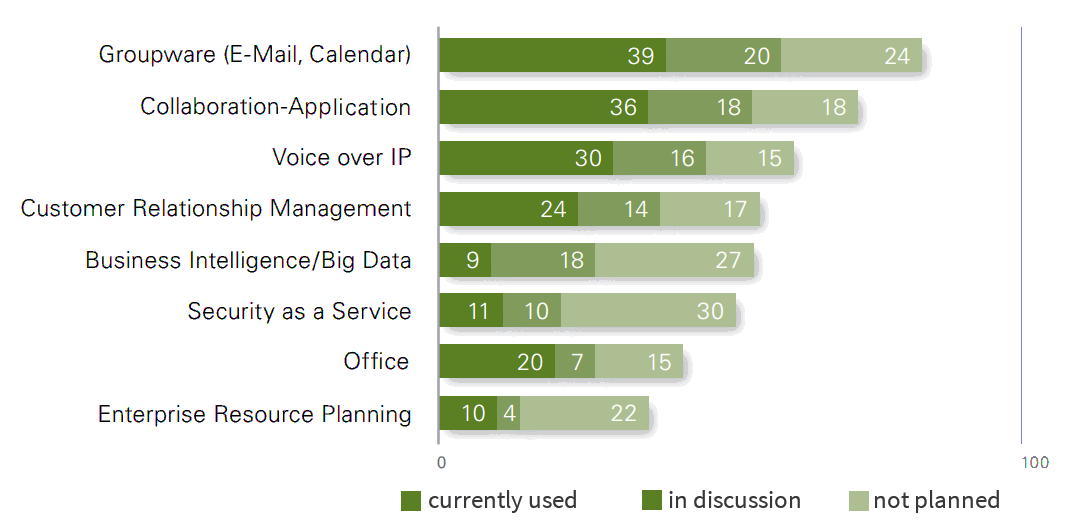
\includegraphics[width=0.75\textwidth]{images/cloud_application_germany.png}
%	\caption{CollaboraTeX form to import \LaTeX documents}
% \end{wrapfigure}

\chapter{Introduction}
Cloud Computing is a longstanding trend in Information Technology (\abk{IT}{Information Technology}) that quickly gained attention of decision makers and companies around the world once its full potential was realised. The key promisings of Cloud Computing are increased flexibility, better effectiveness of shared resources, less maintenance and significantly reduced costs.

It enables companies to outsource its technologies on different layers and migrate them to the services of Cloud providers. Today, \nameref{subsubsec:saas} is the most widespreach Cloud service, with 73\% of companies using it, followed by \nameref{subsubsec:iaas} with 47\% and \nameref{subsubsec:paas} with 33\%, according to a study by Gartner that consulted 2.300 Chief Information Officer (\abk{CIO}{Chief Information Officer}) worldwide \cite{website:gartner-cio-survey}.

Companies are increasingly relying on Cloud Computing and when considering the different \nameref{subsec:cloud-deployment-models}, there is clear evidence that hosting their private Cloud is equally important to them as the utilisation of other Cloud provider's services. At the same time, public services are much less common.

\begin{figure}[H] % \todo{vor Druck ändern -> h!}
	\centering
		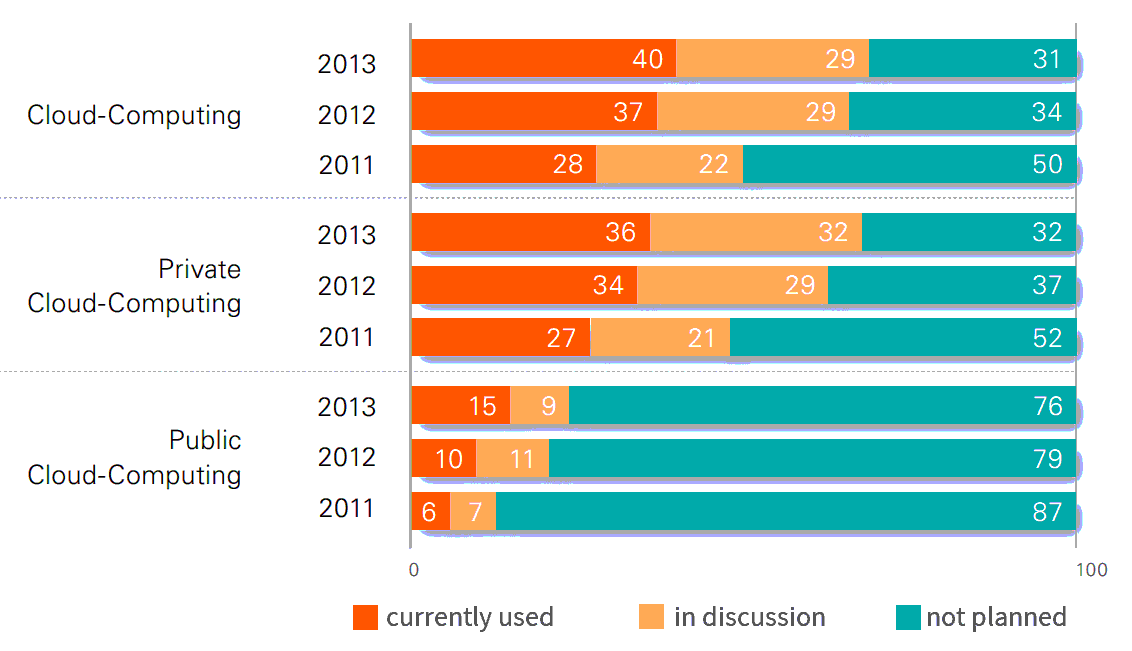
\includegraphics[width=0.8\textwidth]{images/cloud_usage_germany.png}
	\caption{Dominance of different Cloud \nameref{subsec:cloud-deployment-models} in the German market \cite{kpmg2014cloud}}
\end{figure}

As \nameref{subsubsec:saas} is the most important among all Cloud services for companies, the actual usage scenarios are regarded in the following. The most frequent form of using an application in the Cloud are groupware products, such as email and a calendar, followed by collaborative applications. More than half of all companies are currently utilising these tools.

The other two vital applications are Voice over IP and Customer Relation Management (\abk{CRM}{Customer Relation Management}) applications, while of the rest, Business Intelligence/Big Data, Security as a Service, Enterprise Resource Planning and Office, the latter is to be mentioned as still somewhat relevant.

\begin{figure}[H] % \todo{vor Druck ändern -> h!}
	\centering
		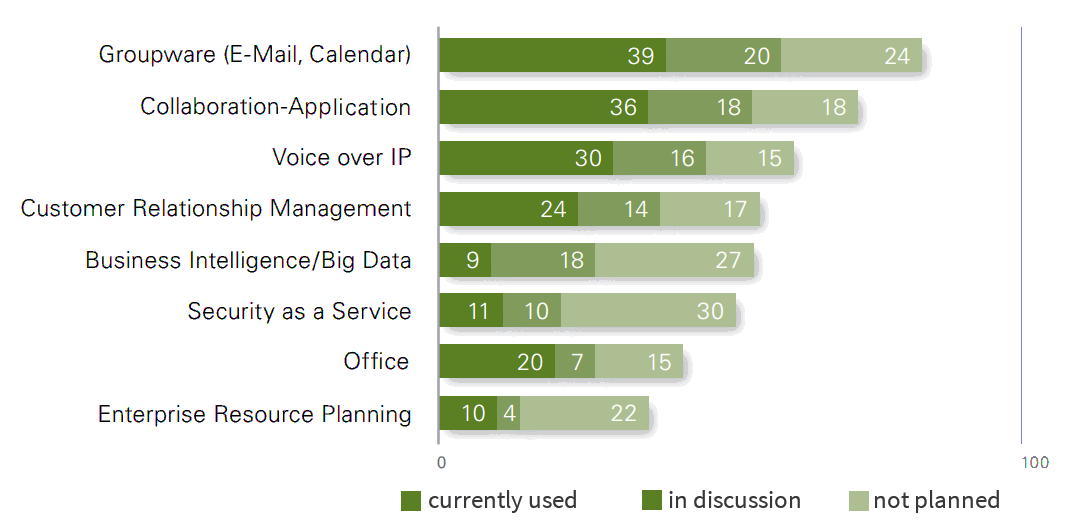
\includegraphics[width=0.85\textwidth]{images/cloud_application_germany.png}
	\caption{Different usage of \nameref{subsubsec:saas} in companies \cite{kpmg2014cloud}}
\end{figure}

And the majority of companies are quite satisfied with their experiences, 44\% of them perceive it as positive in every respect, 39\% as rather positive and only 17\% have a neutral opinion about their lessons learned.

However, as with everything in life, there is also a downside to the operation of Cloud Computing services and all its promises. In June 2013, it was revealed that the National Security Agency (\abk{NSA}{National Security Agency}) of the United States of America is wiretapping all major Internet companies with their top-secret \name{Prism} program \cite{website:guardian-prism}. It has been in operation since 2007 and is aimed to obtained direct access to the servers of Google, Facebook, Apple, Yahoo, Microsoft and others. 

This changed things on dramatic scale. It was previously known that American companies are legally obliged under US law to hand over data of their users, but the direct and unsupervised access of intelligence agencies to the companies' services is yet another dimension. It was disclosed by former employee Edward Joseph Snowden who cited the defence of information freedom as his main motivation \cite{website:guardian-snowden}.

Today it is known that the extent and nature of this surveillance by the NSA even exceeds the initial assumptions and there is even physical access to server hardware that it is being shipped by the manufacturer to its customer \cite{website:nsa-cisco}.

The teachings of this NSA scandal shaped the view of customers and companies for the Internet, its services and Cloud Computing. The confidence in the safety of data and the prevention of unauthorised access are nowadays the two major obstacles in companies to implement Cloud Computing services, stated by 57\% and respectively 71\% of all interviewed companies in Germany.

This shows immediate effect on the IT landscape, as half of the German companies already using or contemplating Cloud Computing are increasing their security requirements or even postponed or abandoned concrete projects.

\begin{figure}[H] % \todo{vor Druck ändern -> h!}
	\centering
		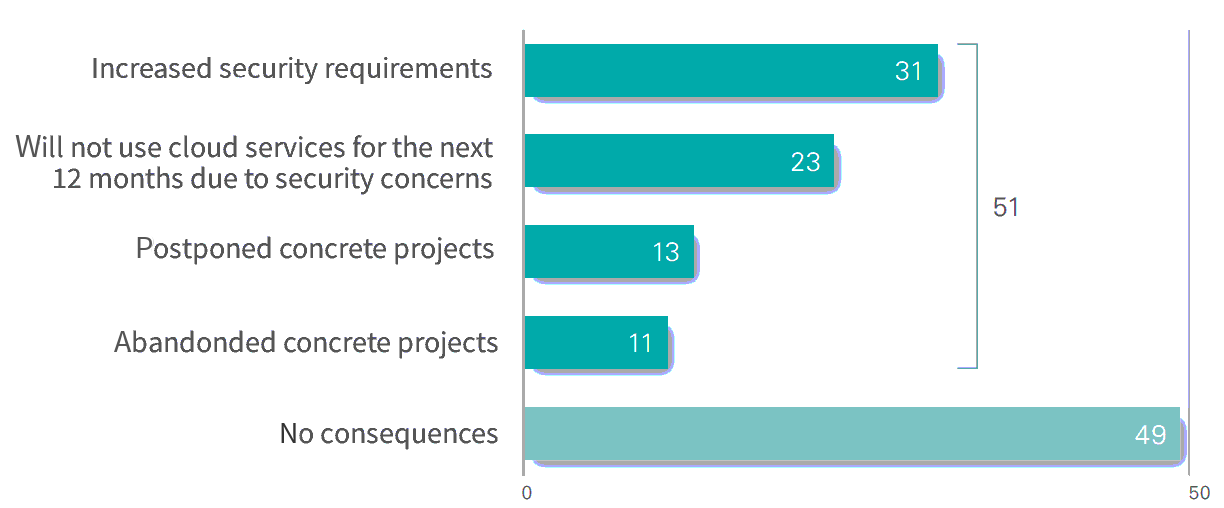
\includegraphics[width=0.9\textwidth]{images/cloud_nsa_consequences_germany.png}
	\caption{Consequences of the NSA scandal on the Cloud Computing strategies of German companies \cite{kpmg2014cloud}}
\end{figure}

It also makes politics appear on the scene. Revocation of the so-called \name{Safe Harbour Argreement}, that allows the legal transfer of individual-related data for European companies to the USA, was discussed by the European Parliament \cite{website:eupa-safe-harbour}. The NSA scandal and the teachings was also one of the major topics of the European elections in 2014. 

Simultaneously there are more and more potential security risks and sources of nonconformances are discovered, as the \name{Heartbleed} bug proved recently. It is a serious vulnerability in the OpenSSL cryptographic software library, which is prevalent on the Internet. The weakness allows the stealing of protected information that are usually encrypted by SSL/TLS and all major web server and operating systems are affected \cite{website:heartbleed}.

On the contrary, data are getting increasingly important for Internet companies, as the other new cool kid on the block besides Cloud Computing, \name{Big Data}, is another trend in IT. It underlines the old proverb \textit{"if you're not paying, you're the product"} as data embody a real business value for companies nowadays.

The numbers of companies and users with security concerns that scrutinise this business model however increases. Due to popular demand, private Cloud Computing is on the rise and ipso facto the premise of this work.

\pagebreak

\section{Scope and Aim}
\label{sec:scope-and-aim}

The idea to this work originates from two main factors. One of the major research areas of the Institute of Telematics (\abk{ITM}{Institute of Telematics}) of the University of Lübeck is Cloud Computing. It is this topic that the PhD thesis of Klaus-Dieter Schumacher focuses on: 

\begin{quote}
Forschungsgegenstand ist die Analyse der Möglichkeiten des Einsatzes von privaten Clouds im universitären Umfeld. Dabei soll auch untersucht werden, in welchem Umfang die in der Universität in den diversen Pools vorhandenen PCs für die Cloud genutzt werden können. Des Weiteren soll evaluiert werden, ob und in welchem Umfang im Rahmen einer Stiftungsuniversität Clouddienste anbietbar sind und durch dritte genutzt werden kann.

In einer ersten Testphase sollen ausgewählte Anwendungen implementiert und zunächst institutsintern angeboten und evaluliert werden.
\end{quote}

So on the one hand, a fully matured application that utilises the exisiting infrastucture is needed by the ITM. On the other hand, there is also a longstanding demand for a software that is capable of the collaborative editing of \LaTeX documents. With such an application it would be much easier for the staff to work on scientific research papers, academic exercises, exam papers and so on.

This leads eventually to the aim of this work: To develop a collaborative real-time \LaTeX editor that runs on the Cloud Computing infrastructure of the Institute of Telematics and provide the staff with the ability to work collaboratively on documents.

There was a exisiting solution to this problem, \name{\nameref{subsec:flylatex}}, but it was deemed as insufficient. However in the middle of this work, there was yet another, more mature application released as open source software, \name{\nameref{subsec:sharelatex}}, after already existing as closed source for several years. While it might have satisfied the requirements that were postulated by the members of the institute (compare chapter \ref{subsec:software-requirements}), it could not have been hosted the institute's existing infrastructure (compare chapter \ref{subsubsec:computing-resources}), therefore this work redevelops such a Software as a Service from scratch.

\section{Outline of this work}

This work is divided into five chapters. After the introduction into the topic, an explanation of the scope of this work will be given, followed by the overview of the conventions.

The second chapter will then illustrate the necessary theoretical foundations of \nameref{sec:cloud-computing} by illuminating its \nameref{subsec:cloud-history} and \nameref{subsec:cloud-standards} as well as \nameref{subsec:cloud-deployment-models} and \nameref{subsec:cloud-service-models}. Subsequently, \nameref{sec:collaborative-software} and its distinction to \nameref{subsec:collaborative-editing-foundations} will be reviewed and also the major algorithm behind it, \nameref{subsubsec:operational-transform}.

\pagebreak

In chapter three, existing online \LaTeX editors are reviewed and afterwards the \nameref{subsec:technical-constraints} and \nameref{subsec:software-requirements} elicited. Finally, the findings are analysed and presented.

The fourth chapter is dedicated to the \nameref{chap:architecture} resulting from this work. First of all, the \nameref{sec:approach-and-decision} is elucidated, before presenting the actual design in the respective subchapters Model, Services, Implementation and Tests.

The fifth and last chapter offers the conclusion of this work. It consists of an overlook of the \nameref{sec:implemented-functionalities}, succeeded by the consideration of possible following works and future additional implementations in the \nameref{sec:outlook}.

\section{Conventions}
As this work references various different technologies, applications, file formats, languages as well as classes, methods, packages and parameters, there are typographical conventions that will be followed thoughout this work.

\begin{table}[H]
	\begin{center}
		\setlength\extrarowheight{3pt}
		\begin{tabular}{ m{6cm} | m{3cm} }
		  	\textbf{Typographical Conventions} 	  & \textbf{Applies for} \\
			\hline                       
			\package{de.uniluebeck.package} 	  & Packages \\
			\class{Classname} 					  & Classes \\
			\method{Methodname} 				  & Methods \\ % (including such for the HTTP protocol) \\
			\parameter{Parametername} 			  & Parameters \\
			\parametertype{Parametertype} 		  & Parameter Type \\
			\parametertype{Mediatype} 		      & Media Type \\
			\fileformat{.abc}		   			  & File Formats \\
			\name{Name} 			  			  & Names \\
		\end{tabular}
		\caption{Typographical conventions of this work}
	\end{center}
\end{table}

This example shows how a REST service is specified: 

\restwithparam{description}{method}{url/\{urlParam\}}{ConsumeMediaType}{ProduceMediaType}{param}{paramType}{returnType}

\pagebreak

Source code examples are following the conventions of their respective language. For the programming language \name{Java}, the code conventions defined by Sun Microsystems and retained by Oracle, apply \cite{website:java-conventions}.

This work was developed under the agile process model, using Netbeans as \abk{IDE}{Integrated Development Environment} and the Java Development Kit in version 7, Update 51.


	\chapter{Foundations}
This chapter illustrates the basic principles of \nameref{sec:cloud-computing}, \nameref{sec:tex} and \nameref{sec:collaborative-software}. Additionally, it focusses on the specialities of \nameref{subsec:collaborative-editing-foundations}, the as well as the \nameref{subsubsec:operational-transform} algorithm in theory, practice and the necessary knowledge for the implementation of undo and redo with it.

\section{Cloud Computing}
\label{sec:cloud-computing}

An overview over the theoretical foundations, underlying principles and technologies of Cloud Computing will be given in this chapter. It starts with a brief introduction to the characteristics and is then looking at the different deployment and service models of Cloud Computing, \nameref{subsubsec:iaas}, \nameref{subsubsec:paas} and \nameref{subsubsec:saas}. 

Regarding these service models, the infrastructure of the Institute of Telematics' private cloud will be briefly outlined afterwards, before ending the chapter with basic foundations of collaborative software and the specifics of collaborative editing, including standard algorithms.

\subsection{History}
\label{subsec:cloud-history}
The history of Cloud Computing is inseparably connected to the one of large-scale computing in computer science and can be viewed as a wavelike expansion over time. It started with rapid initial growth, then went into decline and is now surging to new heights.

\begin{figure}[h!]
	\centering
		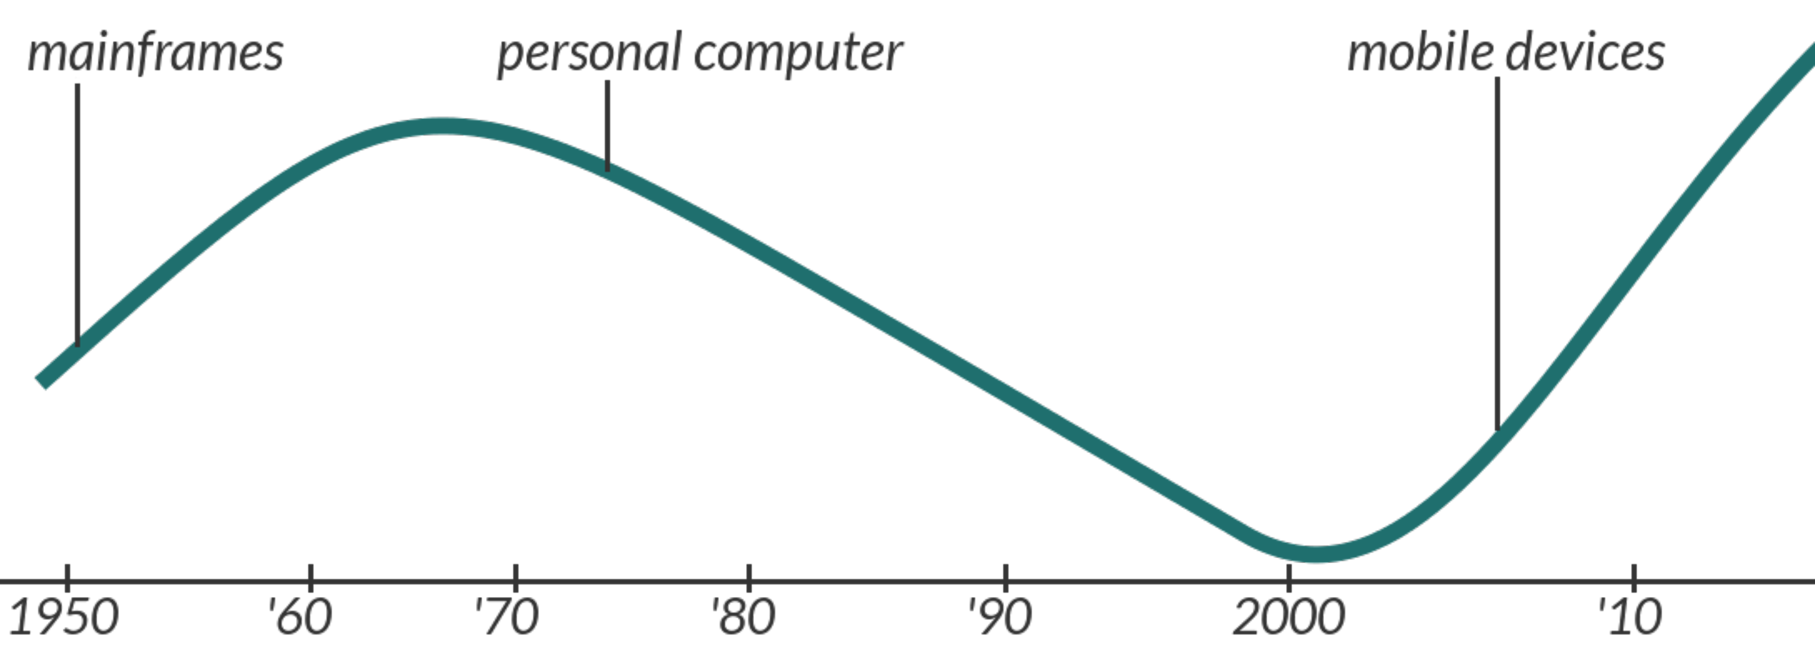
\includegraphics[width=0.8\textwidth]{images/computing_expansion.pdf}
	\caption{History and prevalence of large-scale computing over the decades}
\end{figure}

In the early days of computing, the 1950s and 1960s, large-scale mainframe computers where used in public constitutions such as universities, military research facilities and business companies around the globe, commanding them on terminals. In that period, they reached their all-time peak for the time being and in the following decades, the success of the personal computer led to their steady decline and the belief, that the future of computerisation is personalised. This is turning out to be very true. 

The roaring growth of the Internet and its ubiquitous use on mobile devices gave large-scale computing a comeback, with data centers nowadays representing the backbone of major Internet companies and enabling recent technological approaches like Big Data or Cloud Computing.

In the foreseeable future, this development is even going to speed up as more and more people are connected to the Internet and previously local applications for the computer are now being provided as services and shifted into the cloud, for instance Photoshop, which is now available only via the Adobe Creative Cloud \cite{website:adobe-shift-cloud} \cite{website:adobe-photoshop-cc}. But the pioneers of Cloud Computing where other companies.

The rise of Cloud Computing can be seen as an aftermath of the New Economy. After its demise, companies had to reinvent themselves to survive the struggle for customers and draw several lessons from it \cite{bitkom2012soacloud}:

\begin{itemize}
	\itemsep2mm
	\item{Competition is universally in the Internet and each competitor is always just a single click away. Customers are product- and not vendor-loyal, always on the look for the most innovative, easy to use and especially cheap provider. Such with comfortable, attractive and intuitive user interfaces have a competitive advantage.}
	\item{Customers are very sensible to fluctuations in the quality of service. Amazon had to learn that a 1/10 of a second slower response time can already lead to a decrease in revenue by 1\%, while Google noticed the same for search requests, with a 20\% drop if response times slowed down by 0.5 seconds.}
	\item{If a product will find a ready market, demand exceeds supply rapidly and only massive-parallel IT infrastructures have the potential to scale accordingly on short notice. Software must developed agile and interchangeability of a component-based software architektur is a must, making permanent innovation possible.}
\end{itemize}

Google and Amazon where the first companies to react to these new challenges, both in their own way.

After the end of the boom, companies had difficulties to acquire money for their growing businesses, as angel investors were cautious and venture capital has become scarce. Google adapted to it by using only hardware from low-budget computers, interconnecting them to a heterogenous, massive, parallel computing archictecture, promising endless extensibility. 

\pagebreak

Using this type of infrastucture resulted in several non-trivial problems, as parallel architectures can merely scale if software components share nothing, and Google solved them by software \cite{lee2011sharednothing}. For this, a particular database \name{Google Big Table} was developed as well as fault-tolerant software, leading to the invention of the established \name{MapReduce} algorithm \cite{dean2004mapreduce}. 

This infrastucture emerged to be extremely cost-efficient and was copied by various other companies, nowadays being the blueprint of massive-parallel architectures and Cloud Computing.

Contrary to Google, Amazon was part of the Internet boom and invested enormously into its infrastructure during that time, building up huge, unused capacities. To make use of its bloated infrastructure, Amazon decided to rent it out to other companies. This move, initially being born out of pure economical necessity, made Amazon the first real service provider, awarding itself with a lucrative revenue stream besides its main business. But unknowingly, it also laid the second cornerstone for Cloud Computing. 

In the wake of early success, Amazon constantly evolved the new business model and formed an independent branch with cloud services, now known as \name{Amazon Web Services} (\abk{AWS}{Amazon Web Services}), which today significantly contributes to the company's operating income.

The aforementioned developments, made by both companies independently of each another, transformed the IT landscape permanently as others learned how to use Google's and Amazon's game changing ideas for their purposes which led to the creation of the Cloud Computing industry.  

At that time, the term Cloud Computing was also coined. It derives from the common practice to model the Internet as a cloud-shaped drawing in network diagrams \cite{hausman2013cloud}.

\subsection{Standards and Characteristics}
\label{subsec:cloud-standards}
While Cloud Computing is ubiquitously used nowadays and considered an industry standard, no distinct and universal definition emerged over the years. However, the United States National Institute of Standards and Technology (\abk{NIST}{National Institute of Standards and Technology}) published a definition in 2011 that is widely regarded as most important publication on this topic and effectively considered as reference standardisation \cite{mell2011nist}. 

Following the publication of the definition, the NIST layed out a road map for the creation of an official standard, which was published in July 2013 in its most recent version and contains contributions from members of the NIST themselves as well as other universities and several industry partners such as Oracle or Microsoft \cite{sokol2013nist}. Furthermore, a conceptual reference architecture was published in 2011, which defines not only roles, technological and architectonic aspects, but also quality and orchestration of services. 

\begin{figure}[H]
	\centering
		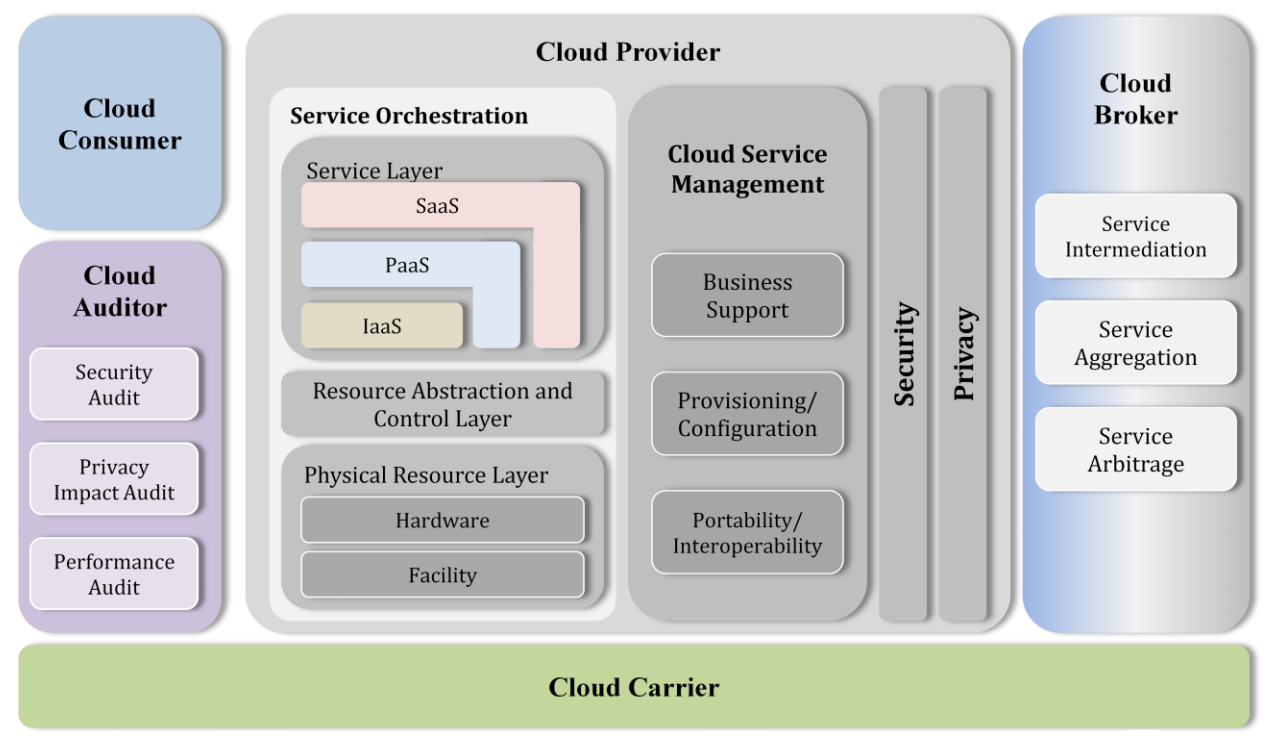
\includegraphics[width=0.85\textwidth]{images/cc_conceptual_reference_model.png}
	\caption{The conceptual reference model of the NIST \cite{liu2012reference}}
\end{figure}

As this broad approach aims to cover for all possible platforms and conceivable uses, there will only be a brief explanation of the most important parts of the reference architecture for this work, which essentially condenses to \name{Services Orchestration}. That term refers to the coordination and management of software and hardware resources for the provisioning of holistic cloud services to consumers.

\begin{figure}[H] % \todo{vor Druck ändern -> h!}
	\centering
		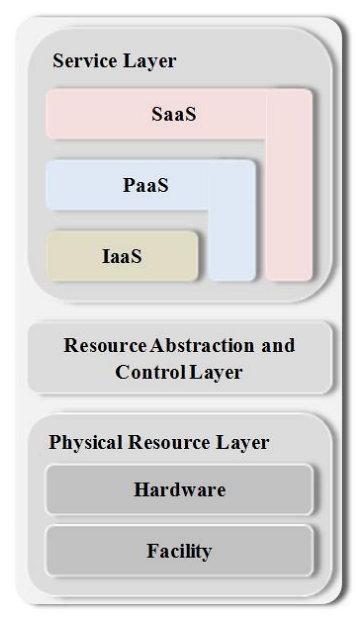
\includegraphics[width=0.275\textwidth]{images/cc_reference_part.png}
	\caption{For this work relevant part of the conceptual reference model of the NIST \cite{liu2012reference}}
\end{figure}

The \name{Services Orchestration} model consists of three different layers, the \textit{service layer}, the \textit{resource abstraction and control layer} and \textit{physical resource layer}, expressing the dependency and abstraction between these. From top layer to bottom layer, each component bases on the one from the contiguous lower layer, while the one's from the lower layers cannot directly access the one's above them.

Representing the top of the model, the \textit{service layer} is defining the interfaces that cloud consumers interact with when they are using cloud services. The single layers are explained profoundly in chapter \ref{subsec:cloud-service-models} in the section \nameref{subsec:cloud-service-models}. Regarding this model however, it is necessary to know that it is possible but not required that the layers are built on top of one another, therefore these are shown as components stacking on each other while being seperate layers. That way, a \nameref{subsubsec:saas} can either be built on top of a \nameref{subsubsec:paas} or hosted on a self-provisioned infrastructure.

The middle layer, \textit{resource abstraction and control layer}, contains system components that providers use to let others access the underlying physical resources. It ties together the various resources and their software abstractions and serves as middleware. The additional \textit{control} aspect refers to access control, monitoring and usage supervision.

The \textit{physical resource layer} includes generally all hardware related infrastructure and resources but exceeds the simple provisioning of CPUs, memory and data store by far. It also involves all physical elements such as power, cooling, maintenance and other aspects.

Given this model and it's layers, only the first can be considered really relevant for this work, as the final application will be a \nameref{subsubsec:saas}, relying on other technologies and middlewares, such as OpenStack, managing the physical resource layer. Although the other layers are used as well, they are much less of a concern, only abstracting resources for the top layer on the sake of easier utilisation.

As previously stated, a definition of Cloud Computing was published by the NIST in 2011 and it also stated five main characteristics, namely \textit{on-demand self-service}, \textit{broad network access}, \textit{resource pooling}, \textit{rapid elasticity} and \textit{measured service} \cite{mell2011nist}. \\
While these characteristics are universally applicable, their composition is rather theoretical and there are some aspects missing. For this reason, they are complemented and extended in the following. This is also showing that Cloud Computing shares most characteristics with distributed systems, but has some unique qualities that distinguishes it from other approaches and underlines its superiority towards them.

\begin{description}
	\itemsep2mm
	\item[Agility] \hfill \\
		The flexible provisioning of any resources needed by the customer, offering web interfaces to dynamically self-manage the utilisation of provided services.
	\item[Device Independence] \hfill \\
		Customers must be able to access cloud services with any device, be it laptop, tablet or mobile phone.
\pagebreak
	\item[Application Programming Interface (\abk{API}{Application Programming Interface})] \hfill \\
		Accessibility has not only to be provided for developers but computers as well by creating machine-readable interfaces. Such an API will typically be implemented using Representational State Transfer (\abk{REST}{Representational State Transfer}).
	\item[Costs] \label{item:costs} \hfill \\
		Costs are one of \textit{the} benefits of Cloud Computing and the major sales argument for providers. Previously, an organisation or business had to maintain its own complete IT infrastructure, which was then in fact mostly unused as the available capacity also reflected necessary reserves to meet peaks in demand. Moreover, such an infrastructure meant having dead capital that could not be spent elsewhere. With Cloud Computing, this money is freed-up for businesses, being able to use it on other spendings while having only to pay for the actual use of IT infrastructure and/or services.
	\item[Geographical Diversification] \hfill \\
		Major service providers operate data centers on different locations, often spread over the whole world and all continents. When provisioning their services, the nearest to the customer located site will be chosen to handle all requests, accounting for minimal response times and higher quality of service.
	\item[Virtualisation] \hfill \\
		Targeting to utilise hardware in the most optimal way, it allows infrastructure such as servers and storage to be shared. Virtual machines are abstracting the hardware layer, allowing software to be executed on any host without restraints. This is done by emulating the underlying hardware resources purely in software. That way any guest can be used on any host, running virtual machines with Linux on Windows hosts or the other way around. This is essentially when migrating applications in the form of virtual machines between servers, which is a must for scalability and load balancing.
	\item[Multitenancy] \hfill \\
		Multitenancy is the actual effect of virtualisation, as it means sharing resources and costs amongst multiple service customers. It reflects the centralisation and better average utilization of infrastructure, as explained earlier in Costs.
	\item[Reliability] \hfill \\
		Realiability is not only meant in such a way that provided services are reachable 24 hours a day, seven days a week, but that they also come with absolute fault tolerancy, guaranteeing a 100 per cent uptime for business continuity.
	\item[Elasticity] \hfill \\
		As it is closely related to scalability, it defines the degree to which a system can adapt to changing loads and peaks, dynamically provisioning resources when needed and deallocating them when not. This intelligent load balacing differentiates it from the term scalability, which describes only the scaling itself but not automation of doing so.
	\item[Monitoring] \hfill \\
		Performance, use of services and system errors are monitored. The first one is done for customers to see their systems performance but also for the provider to optimise its systems effencience as well as finding possible faults like memory leaks. The second is used to bill the services and the last to react to failures.
	\item[Security] \hfill \\
		Non-disclosure of a customers data is imperative, as well as guaranteeing their integrity and protection against data loss. These concerns are even more urgent in a multi-tenant environment, as it exists in Cloud Computing. At the same time several Cloud Computing characteristics, e.g. distribution, add to complexity and increase the difficulties of securing these systems.
	\item[Maintenance] \hfill \\
		Maintenance is a cross-cutting concern to assure several, previously mentioned characteristics of Cloud Computing like security, performance and reliability. This can only be achieved when hardware replacements or software updates are completely transparent to the customers.
\end{description}

\subsection{Deployment Models}
\label{subsec:cloud-deployment-models}
When speaking of clouds, publicly available services of large Internet companies come to mind, but it is not imperative for clouds to be public. They can also be private, even so partially, which then makes a hybrid model, as can be seen in the following descriptions.

\begin{description}
	%\addcontentsline{toc}{subsubsection}{Public Clouds}
	\item[Public Clouds] \hfill \\
		Available to the general public, they are owned and provisioned by businesses or organisations, sharing their resources over the Internet, involving web applications and often third-party tools. When billing them, it will be on a per-use basis.
	%\addcontentsline{toc}{subsubsection}{Private Clouds}
	\item[Private Clouds] \hfill \\
		Contrary to the above, a private cloud exists only within the enterprises' or organisation's boundaries, being shielded from the Internet by internal firewall. As most benefits and characteristics of public cloud are shared, this self-management is the major distinction between them.
	%\addcontentsline{toc}{subsubsection}{Hybrid Clouds}
	\item[Hybrid Clouds] \hfill \\
		The combination of public and private clouds, dividing responsibilities between the company or organisation and service provider, is called hybrid. It can be composed of two or more clouds that are their own entities but bound together. Hybrid clouds are often used to ensure privacy, integrity and safety of data by storing them in-house, while relying on public cloud providers for less critical data and services.
\end{description}

\subsection{Service Models}
\label{subsec:cloud-service-models}
With the continuing development and growing maturity of Cloud Computing, lines between the different service models are beginning to fade more and more. Nowadays there is an approach to provide Everything as a Service (\abk{XaaS}{Everything as a Service}), but when looking at Cloud Computing as a stack, there are three different service models that have evolved over the time, depicted by the following graphic. For the sake of completeness and better understanding, clients have been added to it as well.

\begin{figure}[H] % \todo{vor Druck ändern -> h!}
	\centering
		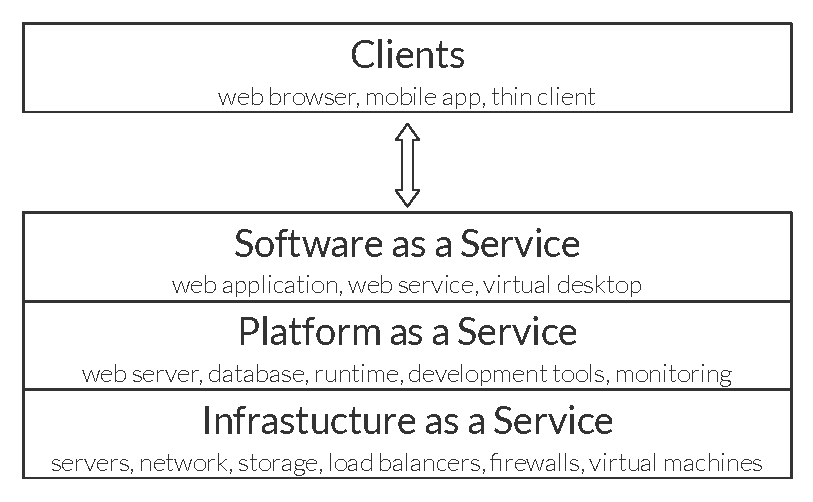
\includegraphics[width=0.66\textwidth]{images/cc_service_models.pdf}
	\caption{The three service models of Cloud Computing}
\end{figure}

While each service model can be used independently and does not require to utilise the underlying model to tender its services, providers often rely on them for reasons of simplification and cost effectiveness. Therefore making it an actual stack, when other as-a-Service's are used.

\subsubsection{Infrastructure as a Service}
\label{subsubsec:iaas}
Being the most low-level of the three service layers, Infrastructure as a Service (\abk{IaaS}{Infrastructure as a Service}) is the cornerstone of Cloud Computing architecture and provides for all hardware needs. It typically includes the provisioning of servers, storage, firewalls, load balancing, interior and exterior network connectivity \cite{mcgrath2012understanding}. In addition to it, all dependent services like monitoring, security, maintenance, but also intangible assets as knowledge and personnel will be taken care of by providers, leaving the service consumer with very few residual tasks on his own.

Major providers also possess geographically diversified services, meaning that a host serving a request will be dynamically chosen in the nearest data center to the service consumer.

\pagebreak

Regarding the technology, Infrastructure as a Service involves not only physical computers but even more so virtual machines, allowing multiple guest systems to share a host and dynamically allocating ressources when needed, therefore reducing costs. The costs are based on the actual resource allocation and consumption, typically ranging from a couple of cents to several dollars per hour \cite{website:aws-ec2-pricing}.

A detailed consideration of underlying technologies can not accomplished this work. Therefore related topics like virtualisation, hypervision, compute instance, resource pooling and so forth will not be addressed further, as the reader is assumed to research these on his own.

\subsubsection{Platform as a Service}
\label{subsubsec:paas}
Providers of Platform as a Service (\abk{PaaS}{Platform as a Service}) offer, as they name states, a platform for others to use. This is more abstract to define than the other service models, but essentially this amounts to the task of provisioning everything it takes to run a specific programming language or technology stack \cite{mcgrath2012understanding}. Typically this includes web server, database, runtime environment, development tools, monitoring. 

This may seem trivial at first. For developing Java applications, for instance, not much more than the \name{Java Development Kit} (\abk{JDK}{Java Development Kit}) including the \name{Java Virtual Machine} (\abk{JVM}{Java Virtual Machine}) and an application server like \name{Tomcat} or \name{Glassfish} is needed, but there are several tasks as dependency management, configuration, maintenance and monitoring to it. It will need to run on an operating system, which will most likely be virtualised as well, relying on the aforementioned \nameref{subsubsec:iaas} or hosted by the provider himself. The complexity of all these challenges are encapsulated by the PaaS provider, being responsible for the immaculate service availability.

Having virtualisation serving as a model where several images can share a host, PaaS providers nowadays do the same within these virtual machines and allocate several applications from different customers, creating a more economic multi-tenant infrastucture.

Platform as a Service also relies heavily on using and serving web solutions, where it can play out it's strengths. \abk{HTTP}{Hypertext Transport Protocol} requests are short-living processes and can be distributed evenly to exisiting servers where they will be processed and then replied to. This is lesser the case for longer running, more resources-demanding jobs, making it not as reasonable to let them run on PaaS environments.

\subsubsection{Software as a Service}
\label{subsubsec:saas}
Software as a Service (\abk{SaaS}{Software as a Service}) is the form of Cloud Computing most commonly known in the general public. Any person being on the Internet will likely have seen it, as all major internet companies provide hosted software for on-demand use. 

\pagebreak

It is typically in the form of an web application, but may also be a web service, a virtual desktop and so on, meaning it is accessed by web browser or thin client. Therefore SaaS can be used from anywhere, anytime, as the only requirement is a working Internet connection.

Using hosted software has multiple advantages. First off, there is no need for customers to install software if they want to use it, it is readily available in the cloud. The same applies for updates, as the service provider always maintains the most recent version of his product. So there is no need for maintenance or support on the customers side, both will be done by the provider. When hiring new staff, the organisation or business will simply need to acquire new licenses, in contrast to the accustomed model where IT has to set up a new employee's computer with all the necessary software and settings \cite{hausman2013cloud}.

This results in total scalability of the applications and the rather sophisticated work behind it is transparent to the customer. When scaling applications, backstage processes first involve cloning and reallocation of virtual machines, then load balancers distribute the tasks to them. Multi-tenancy - as already briefly described in \nameref{subsubsec:iaas} - is broadly used for it as well.

\section{Collaborative Software}
\label{sec:collaborative-software}
Software is described as collaborative if it was designed with the intention to let people work together and achieve common goals, which is sometimes also referred to as Groupware \cite{johnson1990rhythms}. It was defined by Ellis, Gibbs and Rein in 1991 as:

\begin{quote}
	computer-based systems that support groups of people engaged in a common task (or goal) and that provide an interface to a shared environment \cite{ellis1991groupware}
\end{quote}

Its origins can be traced back to the early 1960s when it was envisioned by human-computer interaction and Internet pioneer Douglas Engelbart, who presented it then on the Fall Joint Computer Conference 1968 \cite{engelbart1962conceptual} \cite{engelbart1968human}. This presentation was retrospectively called the \name{Mother of All Demos} as it showcased myriads of inventions that found their way into modern computing. It featured the first computer mouse, a network computer system with real-time text editing and hyperlinks, document version control, a graphical user interface with multiple windows, a predecessor of video conference called teleconference and some more \cite{website:engelbart-1968demo}. When it was connected to the Advanced Research Projects Agency Network (\abk{ARPANET}{Advanced Research Projects Agency Network}) the following year, the first precursor of modern collaborative systems gained an even larger user basis.

Since computer's hardware and connectivity was not ready yet to introduce these developments for personal use and to the general public, more research was conducted, in academia as well as in free enterprise and applications as online chat, video sharing and more were developed further over the next decades.

\pagebreak

With improved technical developments and enhanced maturity of these applications, collaborative software was started to be taken seriously in the beginning 1990s and introduced by the United States government, mainly for military usage. It was also around that time when \name{Lotus Notes} became the first major enterprise application to feature group collaboration and was introduced by several big companies, for instance Pricewater House \cite{website:notes-history}.

As collaborative software was continuously evolving, its next logical step was the migration to the Internet, actively playing a part in the creation and development of what is now known as \name{Web 2.0}, which featured sharing and collaboration as its central resources. That way document sharing, group calendars, instant messaging and video conferencing, amongst other things, were incorporated into applications and websites for the first time and became available to the common user.

\subsection{Collaborative Editing}
\label{subsec:collaborative-editing-foundations}
Collaborative editing is an area of collaborative software where people work together on a problem by making individual contributions. It is divided into several sub-tasks and those are then assigned to either a single person or multiple persons who will work together on one or more tasks.

Such projects are typically more complex in their volume and extent, as is the process of its creation, because collaboration requires coordination between all involved individuals. Besides the actual writing, its structure and the work flow amongst individuals must be also planned and revised and is generally discussed by the whole group.

Collaborative editing is mostly applied for textual documents or source code, asynchronously or in real-time. Such examples for asynchronous collaboration are Wikipedia or version control systems, while Google Docs for instance facilitates real-time collaboration on textual documents. Access management and authentification is essential in both cases but the latter requires even more sophisticated software assistance. 

This software can be a traditional desktop applications, like version control systems, but nowadays more and more applications were migrated to the Internet and are now provided as web applications, like Google Docs. The major technique behind the support for collaborative real-time editing is Operational Transform, which will be explained in the next section.

\subsubsection{Operational Transform}
\label{subsubsec:operational-transform}

Operational Transform (\abk{OT}{Operational Transform}) is the technology for the support of collaborative functions in software systems. It was invented more than two decades ago by Gibbs and Ellis for their GROVE (GRoup Outline Viewing Edit) system and originally designated for the concurrency and consistency control of collaborative editing of text-based documents \cite{ellis1989ccigs}. \\ Nowadays, its collaborative aspect is not limited anymore to the editing of text. As the technology evolved, so did its applications. 

By now it is used for various other tasks as drawing or solving a Rubik's Cube in real-time \cite{website:io2013-drive-api-video}. But capabilities for text-based operations also increased dramatically. Now there is undo, locking, conflict resolution, notifications, sharing and more. It is the core technique behind collaboration features of several major products like Apache Wave or Google Docs.

First, Operational Transform is explained in theory, then an example from real life given and walked through. At last, the specifics of undo and redo operations with Operational Transform are reviewed.

\headline{Theory}
\label{subsubsec:ot-theory}

The foundation of Operational Transform are operations: An action which is to be performed on a data structure - although here it will be focussed on documents. Performed operations on documents are called mutations. The fundamental operations are \method{insert}, \method{delete}, \method{retain} and are more or less self-explanatory. They are used to insert characters, delete characters and move the index by so and so many positions ahead before applying the next mutation.

To handle the concurrent execution of these operations, there is something called \name{transform}, a function that takes two operations, that have been applied on the same document but in different states, from two clients. It re-computes the second operation so that the intended changes of the first operation are preserved and incorporated into the second operation, which can then be applied correctly after taking the first operation into account.

To make this more comprehensible, an extensive example shows the concurrency problems that can appear and the application of Operational Transform to solve them.

\headline{Practice}
\label{subsubsec:ot-practice}

When inserting and deleting locally, it poses no problem to execute these operations as there are no dependent and concurrent operations from other clients that need to be applied.

\begin{figure}[H] % \todo{vor Druck ändern -> h!}
	\centering
		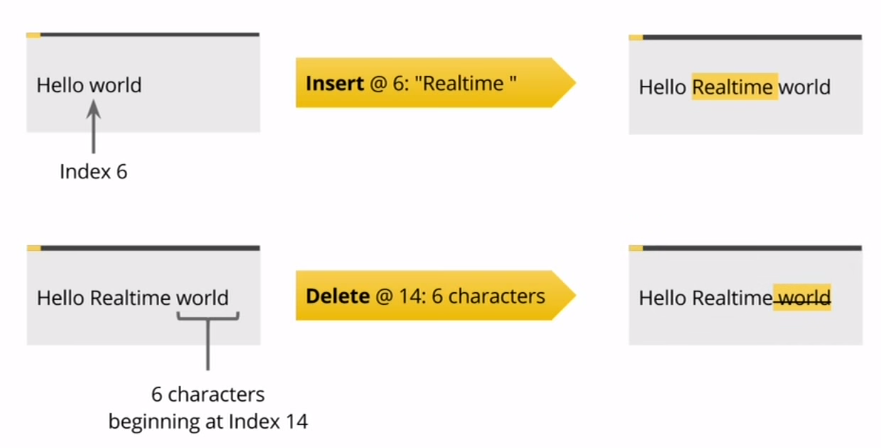
\includegraphics[width=0.75\textwidth]{images/ot_local_insert.png}
	\caption{Local insert and delete of characters \cite{website:io2013-drive-api-video}}
\end{figure}

Synchronising these single local changes between multiple clients is however where problems arise. While editing the same document concurrently, they cannot be simply applied in the order how they would have been locally. This can be seen on the left side of the graphic below. As the second operation is inserted with the local index of the other client, the mutation messes up the document and leaves it in an incorrect state.

The index of the second operation needs first to take the initial operation into account, offsetting its index by the length of the first insert. The re-computed second operation with the altered index position can then be applied correctly, as seen on the right hand side of the graphic below.

\begin{figure}[H] % \todo{vor Druck ändern -> h!}
	\centering
		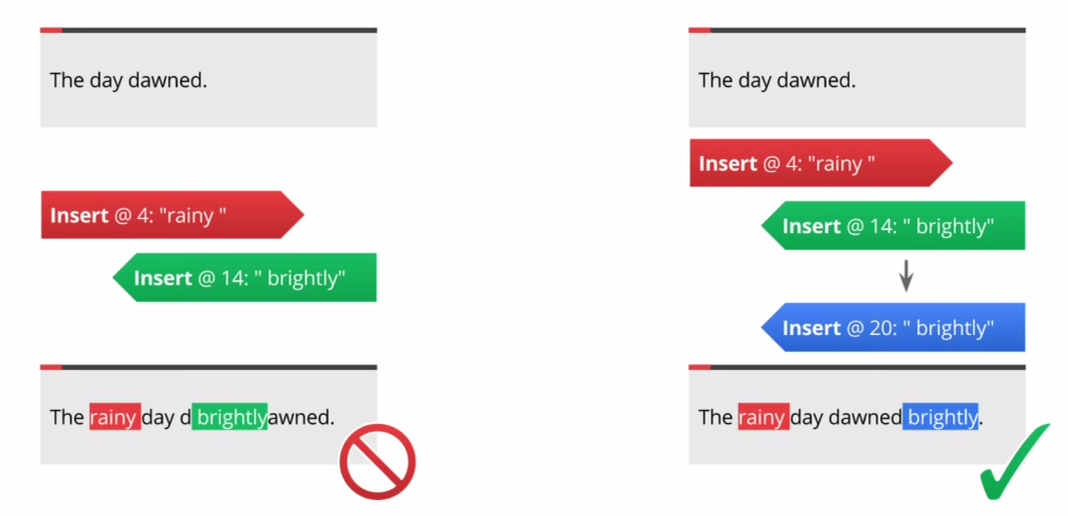
\includegraphics[width=0.85\textwidth]{images/ot_transform_insert.png}
	\caption{Local changes get out of date when other user's changes are incorporated \cite{website:io2013-drive-api-video}}
\end{figure}

What adds to complexity is the transit time of messages. It can lead to further problems when the server, ensuring the transform of operations, is receiving the operations of one client after the ones of another. While all operations can be correctly applied on the client that was sending its operations first, they cannot be on the client whose message reached the server later. Consistency is not achieved in this case.

The problem lies in the processing and transform of operations by the server only. To reflect varying message transit times and being able to handle any incoming operations correctly, regardless of their order and delay, the \name{transform} algorithm also needs to be applied locally. The client must therefore implement the algorithm as well.

\begin{figure}[H] % \todo{vor Druck ändern -> h!}
	\centering
		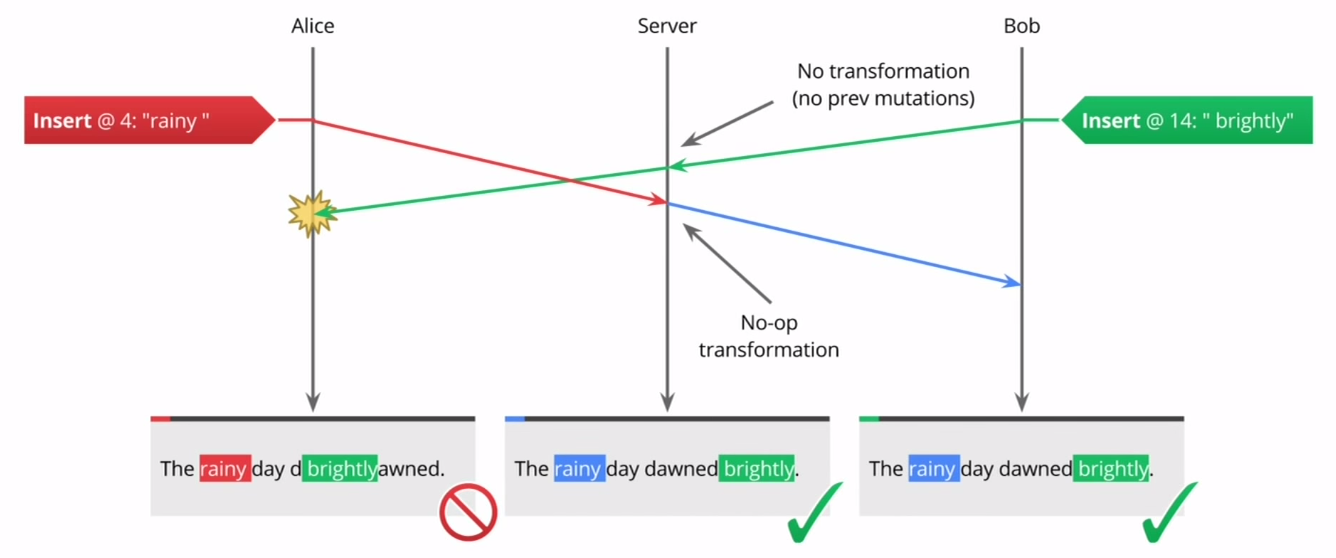
\includegraphics[width=\textwidth]{images/ot_message_transit.png}
	\caption{Conflicts arise when different user operations are performed one after another and their position marks are out-dated \cite{website:io2013-drive-api-video}}
\end{figure}

\headline{Undo and Redo}
\label{subsubsec:ot-undo-and-redo}

For the support of undo and redo of changes made to the document, all operations are pushed to a stack. This holds true for the ones made by the local client as well as those from other collaborators, tracking local and remote changes. The difference however is, that while collaborators' changes are stored unaltered, local changes must be stored with their inverse. For instance, the inverse of an \method{insert} is a \method{delete} and vice versa the inverse of a \method{delete} is an \method{insert}.

\begin{figure}[H] % \todo{vor Druck ändern -> h!}
	\centering
		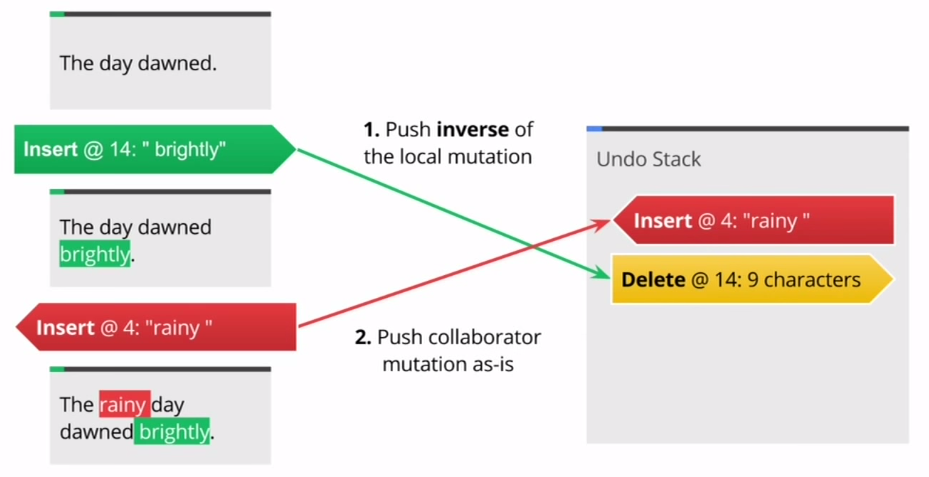
\includegraphics[width=0.75\textwidth]{images/ot_redo_stack.png}
	\caption{All changes are stored on a stack to undo operations in correct order \cite{website:io2013-drive-api-video}}
\end{figure}

\pagebreak

The actual operations and their order on the stack are reasoned by the following: To realise the undo operation, first all collaborator operations are popped from the stack until a local operation is found. The local operation (which is again, the stored inverse of the original operation) must then be transformed against the collaborator's operation to update its index, here shifting it by six positions.

\begin{figure}[H] % \todo{vor Druck ändern -> h!}
	\centering
		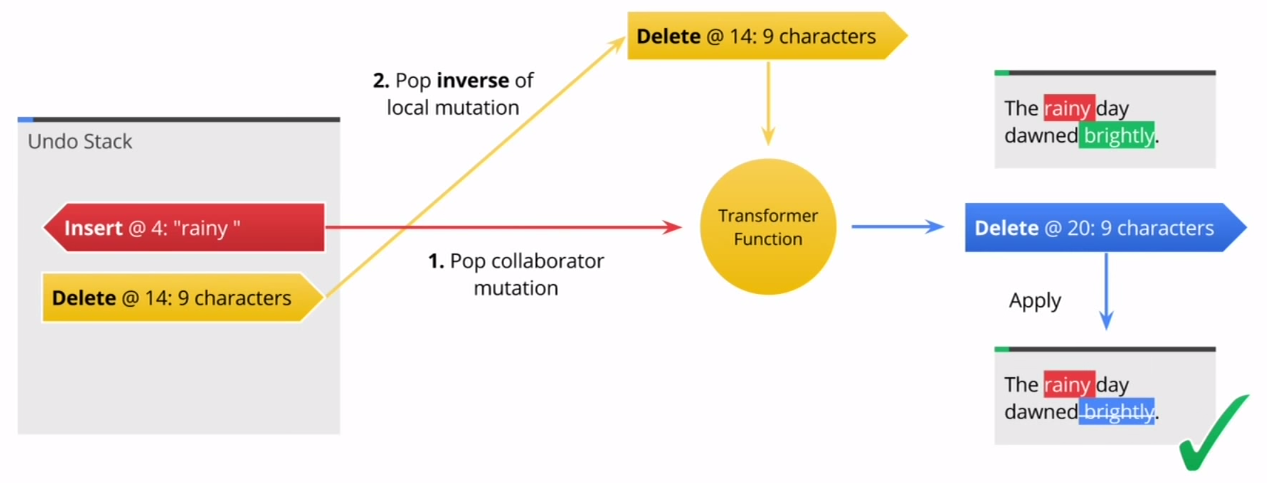
\includegraphics[width=\textwidth]{images/ot_transform_redo.png}
	\caption{For the undo, local changes need to be transformed against remote changes by the transformer \cite{website:io2013-drive-api-video}}
\end{figure} 

\section{\TeX and \LaTeX}
\label{sec:tex}

\TeX is a typesetting system that was invented by Donald E. Knuth in the late 1970s \cite{website:knuth}. It is specifically used for math, technical and other scientific publications, as it contains innumerable amounts of symbols and formulas used in this area, and allows to set the type in outstanding accuracy and quality. It was ultimately developed for Knuth's book series \name{The Art of Computer Programming} and consists of an independent computer programming language and a macro compiler whose source codes were published by Knuth in a computer and operating system independent form \cite{website:tug}.

The output format of a typeset document is \name{DeVice Independent} (\abk{DVI}{DeVice Independent}) and contains positioning directives, references to fonts, type and lines. It is stored, as already stated by the file name, in an device independent form. Before viewing or printing, this format must then be converted into the format of the respective output device, which is nowadays typically a \name{Portable Document File} (\abk{PDF}{Portable Document File}).

As \LaTeX itself is only a macro compiler with relatively few directives that are not sufficiend for most use cases, a set of other macros is needed. Among the most popular set of such macros is \LaTeX which was originally created by Leslie E. Lamport and can be extended by myriads of additional packages \cite{website:dante}.

\pagebreak

The basic macros provide some pre-defined document classes such as article, book, report and slides. There are then possiblibities to structure them further in chapters or sections, with hyperreferences, bibliography, citations, abbreviations and more.

For the conversion to the format of the respective output device, there are so-called engines executing the \TeX format. For example, \LaTeX can be used under \name{PDFTex} as well as under the engines \name{LuaTex} and \name{XeTex}. Although the former is probably the most used, these two are its successors and while \name{XeTex} is considered to be slightly more stable than \name{LuaTex} at the moment, its extensibility might be surpassed by it in the near future.


	\chapter{Current State of Online \LaTeX Editors and the Imposed Requirements on them}
This chapter is aimed at the elicitation of the status quo of other collaborative editors and users' expectations towards them.

First and foremost other existing solutions will be reviewed and then the requirements to a online \LaTeX editor elicited. Finally the elicited requirements and research findings are analysed.

\section{Review of Existing Online \LaTeX Editors}
\label{sec:existing-solutions}
There are two existing solutions, both open source software and can be freely downloaded and installed. They target the same problem as this work, which is providing a collaborative real-time online editor for \LaTeX documents, that is as the same time suitable for self-hosting. 

The first solution, \name{FlyLatex}, is a one-man-project developed by Daniel Alabi and started in 2012, to counter the lack of collaborative real-time \LaTeX environments. It matured until mid 2013, since where there were fewer updates although the project is still being actively developed \cite{website:flylatex-commits}. 

The second solution, \name{ShareLaTex}, originated from a project called \name{ScribTex}, which was the first iteration of an online \LaTeX editor, though not a collaborative one, and published in 2008. \name{ShareLaTex} is the redevelopment and -implementation of that basic concept \cite{website:scribtex} \cite{website:sharelatex}. 

Being run as a website that is free to use for up to two project members but sells subscriptions plans for projects with more members, its code base was published as open source in mid-February 2014, parallel to the draft of this work \cite{website:sharelatex-oss}. 

However, the website continues to be still run as a freemium model, meaning that the basic functionalities are free to use but more extensive features are only available when paying for them.

The architecture and implementation details of each solution will be illuminated hereafter and the findings presented in a nutshell at the end.

\subsection{FlyLatex}
\label{subsec:flylatex}
FlyLatex is developed in Node.js, a lightweight, server-side platform for network applications, built on Google Chrome's JavaScript. It is intended to help implementing data-intensive, fast, scalable applications for real-time applications with its event-driven, non-blocking I/O model \cite{website:node-js}. Moreover, the built-in asynchronous I/O library for file, socket and HTTP communication allows Node.js to act as a stand-alone web server.

Node.js was originally written and initially released on May 27th, 2009 by Ryan Lienhart Dahl. The most recent stable release, as of May 2014, is version 0.10.28.

Node.js' key feature is its performance and concurrency, which works the following way: It uses a cross-platform library that is provided by all major operating systems and abstracts system calls for asynchronous (non-blocking) input/output. Node.js is single-threaded and tells the operating system that it should be notified upon new connections. Right after that, it immediately goes to sleep and when a new connection is made, a callback is executed and the actual work then performed by Node.js.

This results in non-blocking processes, as no function in Node.js is performing input/output operations directly. That way, there are no dead-locks. In addition, it is more memory-efficient in contrast to most other programming languages concurrency models. They usually allocate memory for each new thread and connection, while in Node.js each connection allocates only a small heap.

In short, Node.js excels for thousands of concurrent connections. This is due to the fact that web servers spent a lot ot their time waiting for network or disc access, which is not CPU intensive, and Node.js performs especially well in this area. Thinking in \nameref{subsec:cloud-service-models}, it can be seen as \nameref{subsubsec:paas}, as it also provides a platform to run applications on and shares the suitablity for short-living processes.

But to return to FlyLatex: Being built on the well-illustrated Node.js and written in JavaScript, it makes use of various other technologies such as the \name{ACE Editor}, an embeddable code editor written in JavaScript, that supports syntax highlighting for over 110 languages, code completion and themes among other things \cite{website:ace-editor}. It was developed by Cloud9 for their online IDE and is published as open source on GitHub \cite{website:ace-github}.

To provide collaborative editing, FlyLatex integrates \name{ShareJS}, an operational transform (compare chapter \ref{subsubsec:operational-transform}) library for browsers and Node.js, that adds support for concurrent live editing \cite{website:sharejs}. It was written by Joseph Gentle in 2011, an ex-engineer of Google Wave, which was one of the first major products that featured collaborative editing. But it was closed by Google in 2012, due to the lack of popular demand, and is now an Incubator Project of Apache \cite{website:googlewave-status} \cite{website:apache-wave}. ShareJS is also hosted on GitHub \cite{website:sharejs-github}.

To display Portable Document Files, a viewer called \name{PDF.js} is integrated into FlyLatex. First being started by the Mozilla Foundation as an HTML5 technology experiment that explored building a precise and efficient renderer without native code assistance, it is now officially used in the Firefox browser as default plugin. 

Its major features are a search function, jump to page, zooming, fullscreen view, printing and bookmark support, save as file. Among the extensive features is also the localisation for various languages.

For data storage, FlyLatex relies on \name{MongoDB}, a document-oriented NoSQL database \cite{website:mongo-db}.

FlyLatex is hosted on GitHub \cite{website:flylatex-github}.

After an overview of the technical aspects, the functionalities and implementation will now be discussed. The following features are the ones that FlyLatex describes itself with \cite{website:flylatex-github}:

\begin{itemize}
	\item{Real-time collaboration}
	\item{Real-time status updates on priveleges of documents}
	\item{Online compilation of \LaTeX to \fileformat{PDF}}
	\item{Online \LaTeX debugging}
	\item{Manipulation of compiled \fileformat{PDF}s}
	\item{Sharing of \fileformat{PDF}s}
	\item{Option to use images or additional packages like .sty files}
\end{itemize}

Another point is missing on this list though. FlyLatex can be self-hosted on one's own Node.js server and only requires some configuration for the connection to a running MongoDB instance. This is of major importance, as one must not hand over control of sensitive data and confidential documents to other cloud providers. At the same time, information security is also maximised.

After deploying FlyLatex on Node.js and accessing the webpage in the browser, the landing page shows a login as well as the possibility to sign-up for the service. On successful login, the main page compromises of a simple document management and very basic message center where notifications of changes in documents can be seen. The exisiting documents are listed with their rights (read/write) and can be deleted or shared. New documents can be created as well. 

When sharing documents, the field uses auto-complete on the exisiting users, making it easier to find each individual person. This person then receives a notification, accessible in the message center, and the user is able to either accept or decline the access to the document.

But the core part of FlyLatex is the document editing. The editor comes with syntax highlighting and is displayed full-page. If users edit the document collaboratively, text changes are immediately applied and displayed in other users' browsers that are also working on this document, meaning there is hardly any delay. Although changes are auto-saved they are not persisted in the database, effectively resulting in loss of data when internal server errors occur or it is shutdown, it was just written to volatile memory. Changes are only persisted when explicitly clicking the document's save button.

\pagebreak

To be able to compile documents, the \fileformat{PDF} view must be activated. It provides a button to compile the document, download the \fileformat{PDF} and view the compilation log. The latter is displayed as a small overlay and can be browsed by going back and forth to each log extract. The result of the compilation, the successfully created \fileformat{PDF}, is shown in a preview right next to the editor.

\begin{figure}[H]
	\centering
		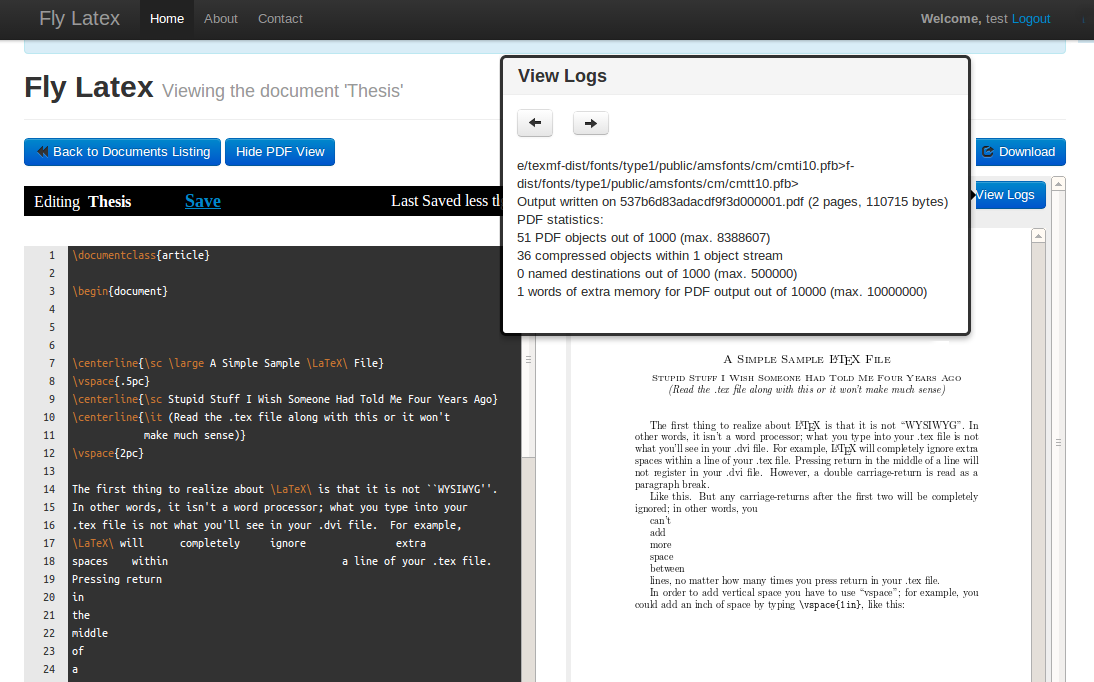
\includegraphics[width=\textwidth]{images/flylatex.png}
	\caption{FlyLatex' document editing and compilation view}
\end{figure}

If there are errors during the compilation, a notification is displayed and the log can be consulted to figure out the cause. When a document was not compiled for the first time, the last successfully compiled \fileformat{PDF} is still shown and the preview not updated.

The actual compilation is achieved by calling the console to execute the transformation of the \LaTeX document. That is why FlyLatex is expecting PDFLatex to be installed, as it is the utilised engine and hard-wired in the source code:

\begin{lstlisting}[language=JavaScript, frame=none, numbers=none, caption=Latex Compilation in FlyLatex]
exec("pdflatex -interaction=nonstopmode "+ inputPath +" > /dev/null 2>&1", 
afterCompile);
\end{lstlisting}

The \parameter{nonstopmode} specifies that the compilation will not be stopped by PDFLatex upon errors, while \parametertype{/dev/null 2>\&1} is redirecting the outputs of the console, resulting in all standard output to be repressed (signifies the compilation log) and only errors being displayed on the console. 

Finally, \parameter{afterCompile} is the name of the callback function that will be executed after successful execution of the command. The actual source code of it will not be listed, but this function reads in the \fileformat{PDF} file and makes it accessible under a unique Uniform Resource Identifier (\abk{URI}{Uniform Resource Identifier}), then reads the log as well and sends both to its own REST services. Finally, it presents the log and file to the user by showing both on the webpage.

Analysing all these information, there are several downsides to this approach:

The handling of documents is rather complicated. To change between documents, one has to go back to the main page and then select a different document to open it. 

A document is a stand-alone file, there is no possibility to structure it by seperating it into more \LaTeX files or include others. That way, bibliography management is not supported as well. 

The log is only accessible in a small overlay dialog and when trying to skip to the end, the next page button must be clicked several times. 

That shared documents have first be accepted or declined in the somewhat hidden message center also adds to the perception of a lacking user experience.

The parallel view of the document and the compiled \fileformat{PDF} is a good approach, but missing controls for zoom. Therefore a detailed examination of the output is not possible for the user, who is left with a rather vague impression about the rightfulness of the created \fileformat{PDF} file.

In conclusion, the bare collaborative document editing and document sharing is working excellent, but advanced functions such as multi-file documents, import, bibliography management and extensive \LaTeX support and tools are missing, preventing a pleasent user experience.

\subsection{ShareLaTex}
\label{subsec:sharelatex}
First and foremost, ShareLaTex cannot be equivalently compared to FlyLatex, as the former is the result of a capital-backed, longstanding project with full-time commitment of its developers. So thinking of ShareLaTeX, the sale of subscriptions makes it actually rather a business model than an open-source project \cite{website:sharelatex-team} \cite{website:sharelatex-subscriptions}. The latter is especially true as FlyLatex used to be the solely available open source online editor, with ShareLaTex being freely available only since shortly, February 2014.

The decision to go open source is justified by the developers in the following way \cite{website:sharelatex-oss}:

\begin{quotation}
As a small team, we're constantly receiving feature requests that we'd love to implement but don't have the time. We've also had a lot of offers from willing volunteers who we've had to turn away because we didn't have a framework for people to contribute. I hope that by open-sourcing ShareLaTeX we can empower our brilliant community to help improve ShareLaTeX in the ways that you want, without having to wait for the two of us to work down our todo list. \\

A lot of people have asked to host ShareLaTeX internally due to company guidelines or data privacy concerns. We don't have the resources to support licensed installs at the moment, but we also hate having to say no. With an open-source version of ShareLaTeX, now anyone who wants to run it locally can.
\end{quotation}

ShareLaTex is hosted on GitHub and consists of several subprojects and services: For the web interface, application of updates on documents, \name{Common LaTeX Service Interface} (\abk{CLSI}{Common LaTeX Service Interface}) for the compilation of \LaTeX documents, \abk{CRUD}{Create, Read, Update and Delete} operations (create, read, update, delete) operations and tracking and storing updates for documents \cite{website:sharelatex-github}.

It mostly relies on the same established technologies as FlyLatex (compare chapter \ref{subsec:flylatex}), such as Node.js, MongoDB, AceEdtior and PDF.js. 

Having said this, it makes use of one additional technology, \name{Redis}, a key-value-store used as data structure server. It is used to perform atomic operations on various data types such as Strings, Hashes, Lists, Sets and Sorted Sets, which are kept as in-memory datasets. Such operations would for instance be: appending to a String, pushing to a List, computing Set intersection, union, difference and so on \cite{website:redis}.

Before running ShareLaTex on Node.js, it must be assured that the Redis and MongoDB services are running, a suitable \LaTeX environment is installed and also a specific version of the \name{latexmk} package.

The \name{latexmk} package can be used in two ways. On the one hand, to detect the correct order and amount of times to compile a document. For example when there is a bibliography and a nomenclature, the execution order would be \method{pdflatex bibtex pdflatex makeindex pdflatex} as the document has to be first compiled. Then the citation references would be set by \method{bibtex}, added to the document in the second compilation step and finally the same would apply for the nomenclature with the last two commands.

On the other hand, \name{latexmk} is even more powerful as it can be used to watch \TeX files for changes and run the necessary commands to re-compile the \fileformat{PDF} automatically.

ShareLaTex comes with several matured functionalities. In addition to the basic CRUD operations, it also supports the inclusion of other files or  even structuring a project with subdirectories. There are various ways to share documents, either with specific users - for which their e-mail has to be entered - or by URI. If the latter is chosen, projects can be made either publicly readable or editable, providing also access to users outside of the platform. Besides, exisiting projects can be download and new projects imported as ZIP file.

There are also specific project settings, as for the spellchecking language of documents, setting the main document and which compiler (PDFLaTeX, LuaTeX, XeLaTeX) to use, whereas some features are exclusively available to the website. Such as the newly introducted integration of DropBox, templates, the help and a \LaTeX tutorial.

\pagebreak

But the centrepiece is the document editing view, which also combines the preview of the compilated \fileformat{PDF} and raw compilation log. There are, from left to right, a foldout sidebar with icons for the code, history, sharing and settings of the document, the project file tree where files can be added, renamed, deleted, the editor containing the document's \LaTeX code and the mentioned preview for \fileformat{PDF} and log.

\begin{figure}[h!]
	\centering
		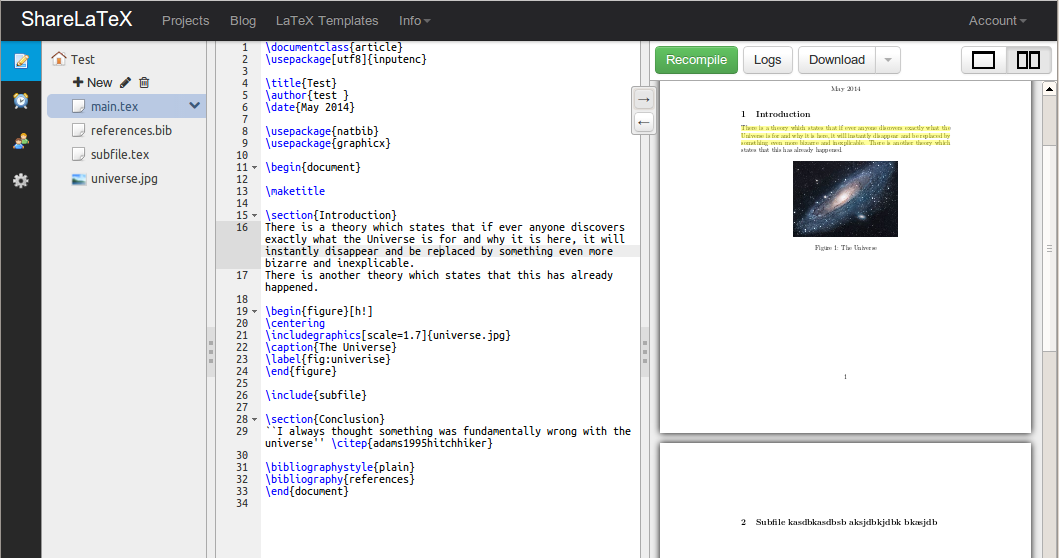
\includegraphics[width=\textwidth]{images/sharelatex-editing.png}
	\caption{ShareLaTex' document editing and compilation view}
	\label{sharelatex-editing-view}
\end{figure}

As ShareLaTex makes use of the same most commonly used and proven library \name{ShareJS} to enable collaborative editing, changes in documents can be seen instantly in other browsers. If a document is edited by several individuals, each user's current cursor position is shown in a different colour to make it clearly recognisable on which part of the document he is presently working. Changes are instantaneously persisted in the database, code completion is provided by the editor.

When there are errors during compilation, they are automatically extracted from the log and presented in summary, with description and cause. As a matter of course the raw log output can be viewed was well.

\begin{figure}[h!]
	\centering
		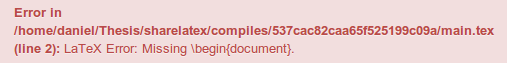
\includegraphics[width=0.66\textwidth]{images/sharelatex-error.png}
	\caption{ShareLaTex' summarises errors with description and cause}
\end{figure}

Document compilation is quick and the preview has, unlike FlyLatex, also zoom buttons to take a closer look at the \fileformat{PDF}. The split view of document code and \fileformat{PDF} can be switched to a single view, where either the editor or preview is shown on the entire screen. The sidebar and project file tree remain displayed though.

A rather sophisticated feature is the possibility to click either on parts of the document to see the corresponding code passages or the other way around, where for any code passage the according output in the \fileformat{PDF} is highlighted in a pale yellow tone (as can be seen on the upper right in figure \ref{sharelatex-editing-view}).

If document changes shall be tracked, there is a history where changes are depicted in a timeline. Each modification is shown with time and the user causing it on a sidebar on the right. When clicking on one of these entries, the document's version as of that point in time is displayed in the editor. User's changes are represented in a different color, actually showing a diff of the document. This is quite helpful to spot changes immediately. With this functionality comes also the option to restore the document back to its state of that given point. All in all, this is equivalent to a basic revision control system.

\begin{figure}[h!]
	\centering
		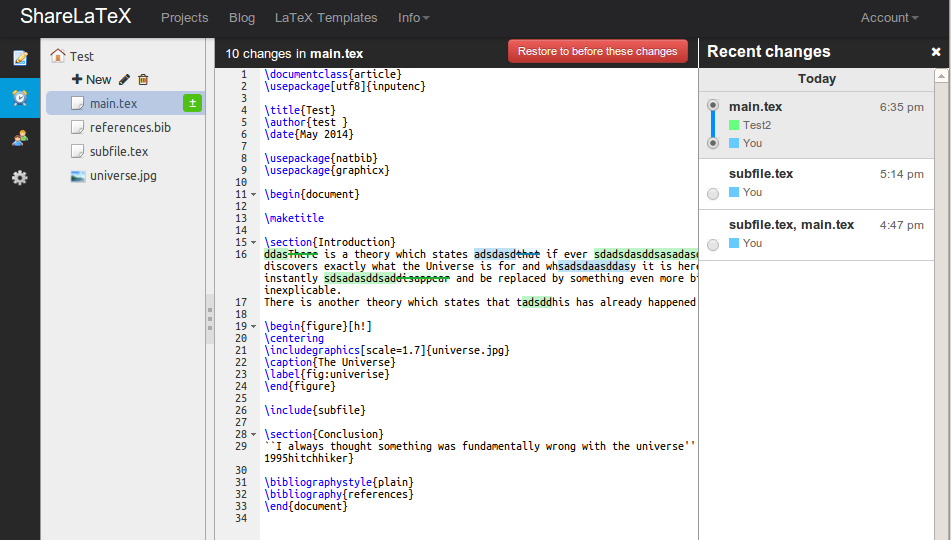
\includegraphics[width=\textwidth]{images/sharelatex-history.png}
	\caption{ShareLaTex' document history view}
\end{figure}

Finally, there are even user settings where the preferred editor theme, font size, key binding can be adjusted, autocompletion switched on or off as well as the user's data and password reset.

The implementation of the compilation is quite similiar to FlyLateX', the process is spawned directly from the command line. Because of the more complex architecture and distributed code base of ShareLaTeX, the actual source code will only be shown in excerpts and for the compilation engine \name{PDFLaTeX}.

\pagebreak

\begin{lstlisting}[language=JavaScript, frame=none, numbers=none, caption=Latex Compilation in ShareLaTeX]
_latexmkBaseCommand: ["latexmk", "-cd", "-f", "-jobname=output", "-auxdir=$COMPILE_DIR", "-outdir=$COMPILE_DIR"]:
return LatexRunner._latexmkBaseCommand.concat(["-pdf", "-e", "$pdflatex='pdflatex -synctex=1 -interaction=batchmode %O %S'", Path.join("$COMPILE_DIR", mainFile)]);
[...]
}).call(this);
\end{lstlisting}

Again, the \parameter{nonstopmode} is used to make the compilation not hold upon errors, as well as a callback function is executed on completion. The major differences are the use of \name{latexmk} (as mentioned earlier a package for automatic document (re-)compilation) and the parametrisation of the compilation engine (here \name{PDFLaTeX}).

Evaluating ShareLaTex' implementation and features, the collaborative nature of its service is ubiquitously noticeable in several functionalities such as the history. It is one of ShareLaTex' strong points, together with document editing, hierarchical structuring, sharing and performance. But there are also weaknesses regarding the support of bibliography and \LaTeX functions, although the latter is partly implemented by the editor's code completion. Nevertheless, ShareLaTex provides a good user experience with all necessary basic functions and even rather useful additional features. 

\subsection{Findings}
Analysing the findings for both existing solutions, \nameref{subsec:flylatex} and \nameref{subsec:sharelatex}, there are several similiarities because of their use of the almost same technologies. 

Both are based on Node.js, which performs and scales very well as lightweight, server-side platform for network applications. It is well-suited as the creation of diffs and application of patches on texts is not very CPU intensive, although the \LaTeX to \fileformat{PDF} compilation is, to a certain amount.

They also share their approach of document compilation: First the command is executed on the console and then a callback function used to process the output further.

Collaborative editing works like a charm on ShareLaTeX and FlyLatex by using ShareJS, there are no noticeable delays and document changes are always applied in the correct way.

Regarding all functions beyond the basics, ShareLaTeX excels FlyLatex in the user experience and the provisioning of useful tools by far. This is obviously the result of long dedication to the project and capital-backed development, while FlyLatex must be seen as what it is: a spare time project of a single developer.

Having been closed-source for most of it's development lifespan, ShareLaTex was a late competitor to the race but is now the leading open-source \LaTeX editor for people or organisations who are dedicated to keep their private data in their own hands. 

However, as can be seen in the next section, neither of the solutions fulfills all requirements for such a collaborative online \LaTeX editor. And above all else, they would also not satisfy the need for an application that utilises the exisiting infrastucture (compare chapter \ref{sec:scope-and-aim} and chapter \ref{sec:approach-and-decision}) of the Institute of Telematics. 

\section{Technical Constraints and Software Requirements}
For the development of a cloud-based \LaTeX editor, there are some technical constraints, predefined by the Institute of Telematics' computing resources, as well as software requirements - be it implicit requirements declared in advance to this work or the one's defined in the preliminary stages by inquiry of the future users.

In the following sections, both contraints and requirements are evaluated to work out the implications for the outcome of this work. First off, the computing resources, topology and technology of the Institute of Telematics' Cloud Computing Lab are treated, then followed by the elaboration of functional and implicit requirements in the next section.

\subsection{Technical Constraints}
\label{subsec:technical-constraints}
The technical contraints consist of various factors such as computing resources, so existing hardware, its arrangement, network topology and ultimately its configuration, especially the systems' architectures, operating systems and middlewares.

These are the variables that will be looked at throughout the following subsections, although it must be noted that only the parts closely related to this work will be reviewed in detail.

\subsubsection{Computing Resources}
\label{subsubsec:computing-resources}
The Cloud Lab's infrastructure is made up of a heterogenous array of computers and servers, ranging from older AMD64 or Intel Core 2 Duo with 2GB of RAM to the new generation of Intel Core i7 with 8GB RAM and therefore reflecting the variances in Cloud Computing systems in a realistic way. 

The topology can be roughly divided into four parts: There are the firewall and the \abk{DNS}{Domain Name System} servers, ensuring network communication and protection of the affiliated systems and then workstations for employees and students. Its most central part though are the different clouds to test a diversity of different infrastructures. 

For such purposes, there are two main clouds, one is based on OpenStack, the other one on Eucalyptus, and then there are two test clouds where more recent versions or new developments in the Cloud Computing landscape can be installed and examined \cite{website:openstack} \cite{website:eucalyptus}. \\
All the mentioned components of the lab can be seen in the network topology below.

\begin{figure}[H]
	\centering
		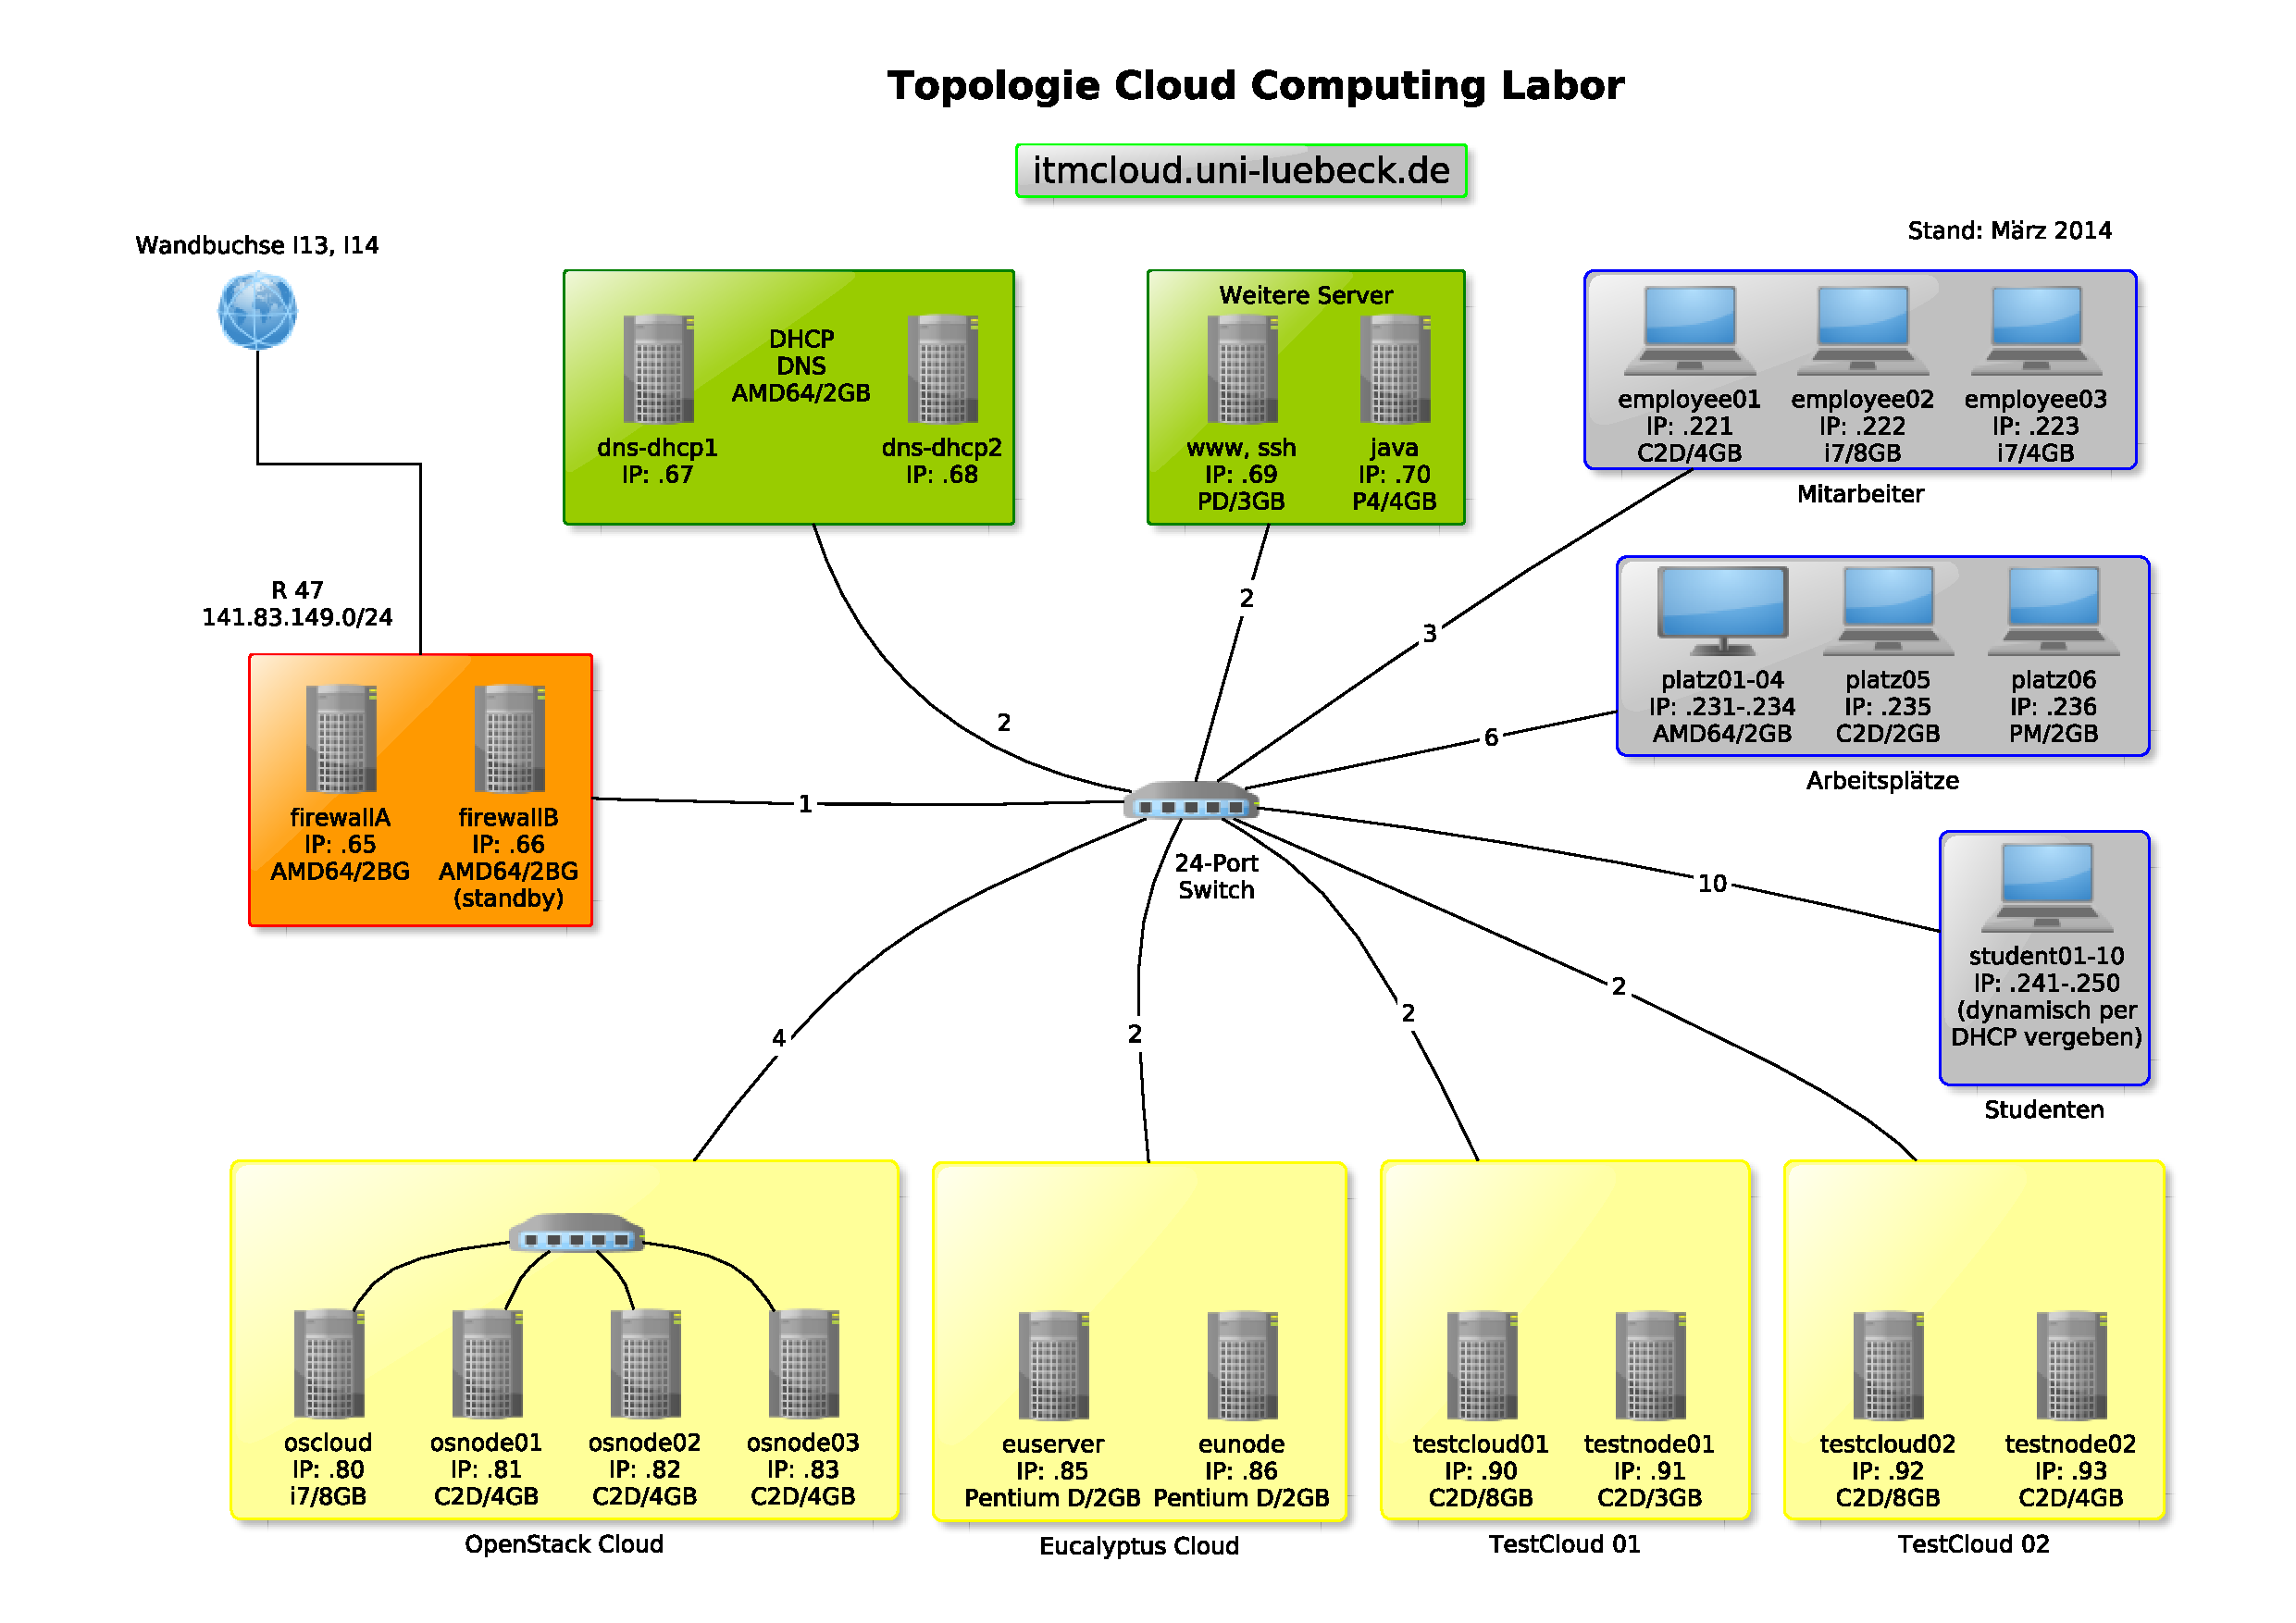
\includegraphics[width=\textwidth]{images/itm-topology.pdf}
	\caption{The topology of the University of L\"ubeck's Institute of Telematics' Cloud Computing Lab}
\end{figure}

Subsequently, only the OpenStack cloud and its characteristics will be regarded as it is the most suitable cloud, which will be explained alongside the depiction of its architecture. For further information on the comparision of different open source Clouds compare the preceding bachelor thesis of Thomas Moritz \cite{thomas2013cloud}.

It should be pointed out that details on the actual configuration are omitted, as this work takes a fully configured and working system as starting point, which is the case with the ITM Cloud Computing Lab.

\subsubsection{OpenStack}
\label{subsubsec:openstack}

OpenStack began in 2010 as mutual project of the NASA and Rackspace Hosting and is now established as non-profit foundation, with many major tech companies like Microsoft, IBM, Oracle or Red Hat being contributers and members of the project. It consists of the components:

\begin{itemize}
	\item{\name{Horizon} serves as a dashboard, a web front-end to manage and control the Cloud and its services}
	\item{\name{Nova} is executing the virtual machines}
	\item{\name{Swift} persists objects and is a highly scalable system where user and instances can store data}
	\item{\name{Glance} manages images and snapshots of virtual machines}
	\item{\name{Keystone} is used for authentification and rights management}
	\item{\name{Quantum} controls the routing and network}
	\item{\name{Cinder} is a block storage that provides logic volumes}
\end{itemize}

The interdependency and relation between these components can be seen in the following graph.

\begin{figure}[h!]
	\centering
		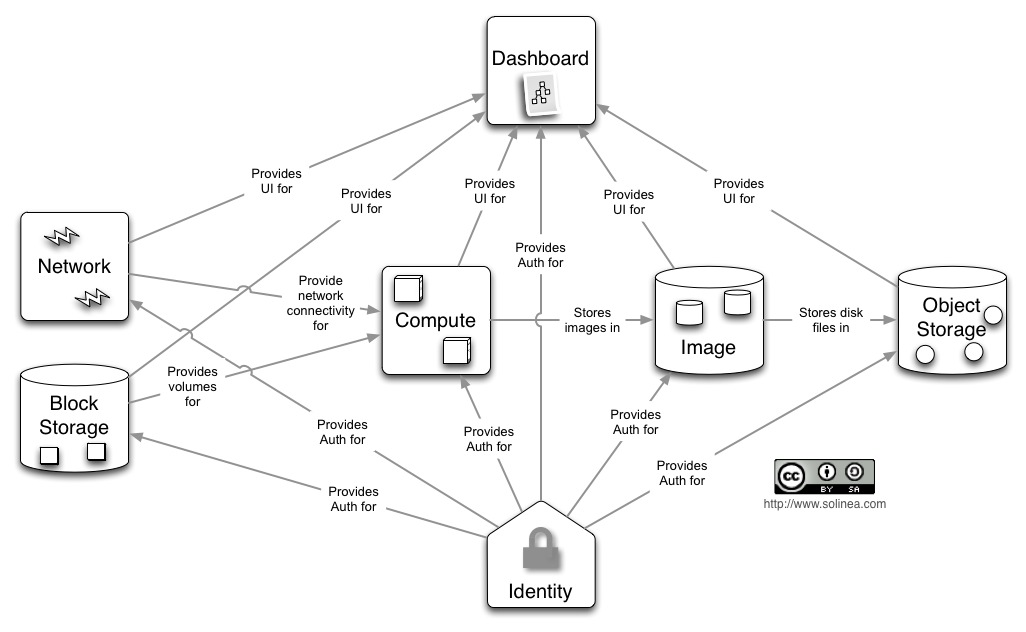
\includegraphics[width=0.9\textwidth]{images/openstack-architecture.png}
	\caption{The architecture and component relations of OpenStack \cite{website:wikimedia-openstack-conceptual}}
\end{figure}

As this is a bit abstract to grasp, there is also a more simplyfied version showing how {OpenStack} provides the basis to build applications on top of it.

\begin{figure}[H]
	\centering
		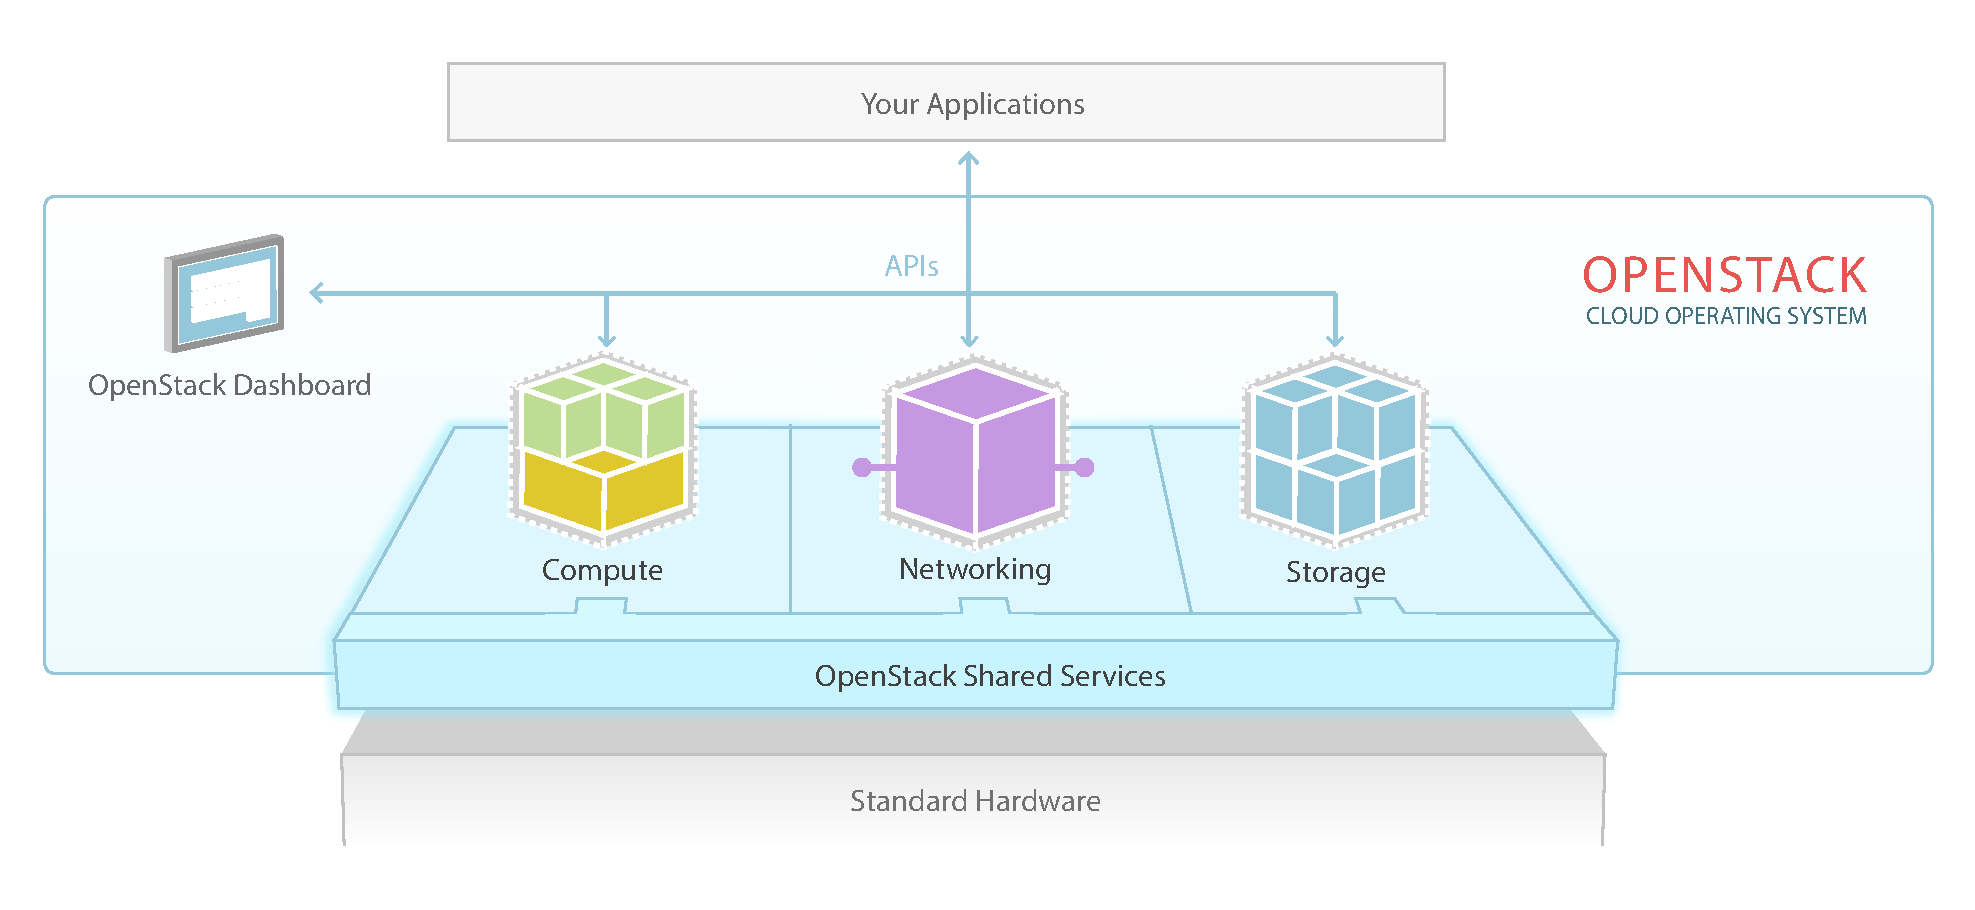
\includegraphics[width=\textwidth]{images/openstack-software-diagram.pdf}
	\caption{Simplyfied OpenStack software diagram \cite{website:openstack-sw-diagram}}
\end{figure}

OpenStack is acting as IaaS and implements simple and massively scaleable cloud services that can be used to provide public or private clouds (compare \nameref{subsec:cloud-deployment-models}, chapter \ref{subsec:cloud-deployment-models}). As can be seen from the graphics, such services include the creation of pools for compute, storage and network resources, which can then be used to virtualise one's server hardware. This happens in a way, that the virtualisation layer abstracts the resource management and specifics of the existing hardware, making both of no concern to the consumer.

The advantages are apparent: While OpenStack is simple to integrate with any hardware, easy to manage and monitor, secure and an industry-wide standard, the systems build on OpenStack are also very elastic, highly available and realiable.

\subsection{Software Requirements}
\label{subsec:software-requirements}
In a software project, requirements engineering, namely the formulation, collection, documentation and maintenance of software requirements, is certainly the most vital part, being not much different for this work. 

There are two main stakeholders, first the users and secondly the operators. While most requirements originate from the users, there were also some requirements couched by the operators. This is potentially leading to conflicts of interest and will be described later, but first all requirements are listed. They are documented as they arised, starting with implicit requirements and followed by the functional ones.

\subsubsection{Implicit Requirements}
\label{subsubsec:implicit-requirements}
There are a number of implicit requirements that were already partially discussed in section \ref{sec:scope-and-aim}, \nameref{sec:scope-and-aim}. These are basic conditions that were defined prior to this work with the supervisor.

To begin with, the application is supposed to run as SaaS. Secondly, it is vital that different users can not only edit documents together but also simultaneously, making the collaborative aspect of the application its most important feature. 

When desired, the current \TeX document has to be compiled and the result shown to the user. Document changes shall be backed by the usage of a version control system that ensures all document revisions are stored and can be restored.

Lastly, access should solely be granted to users of the Institute of Telematics, who will use their exisiting \name{Lightweight Directory Access Protocol} (\abk{LDAP}{Lightweight Directory Access Protocol}) accounts for authentification.

\subsubsection{Functional Requirements}
\label{subsubsec:functional-requirements}
While all these implicit requirements are primarily shaping the architecture of the system, the actual features are defined by functional requirements which are compiled of the later users' requests and needs. 
 
To gather these data, a questionnaire with a list of possible features was prepared. Each functionality could be ranked on a scale from 1, \textit{not so important}, to 10, \textit{very important} and additional remarks or feature requests be made. 

There was a total of 21 questions and a response from 18 individuals, with the highest rating being a 8.7 and the lowest a 4.2. The arithmetic mean was 6.8 and the median 7.0. 

Based on their values, these functionalities were prioritised and divided into three majors groups: \textit{high priority}, \textit{medium priority} and \textit{low priority}. The size of each group was arranged after the arithmetic mean, respectively median, so that the group of highest prioritisation has five functionalities and a arithmetic mean and median of 8.1.

\begin{table}[H]
	\begin{center}
		\footnotesize
		\setlength\extrarowheight{5pt}
		\rowcolors{1}{}{lightgray}
		\begin{tabular}{ p{11cm} cp{1.5cm} }
		  	\textbf{Functionality} 	  														& \textbf{Rating} \\
			\hline
			Undo/Redo of edits																& 8.7 \\
			Support of bibliography/BibTeX management										& 8.3 \\
			Viewable log of the compilation													& 8.3 \\
			Automatic background save while editing (e.g. every five minutes)				& 8.1 \\
			Tabs for multiple opened documents and parallel editing							& 8.0 \\
		\end{tabular}
		\caption{Functionalities with high priority}
		\label{tab:high-priority}
	\end{center}
\end{table}

While the group with medium priority has the same arithmetic mean and median as the overall results of 6.8 and 7.0, consisting of six priorities.

\begin{table}[H]
	\begin{center}
		\footnotesize
		\setlength\extrarowheight{5pt}
		\rowcolors{1}{}{lightgray}
		\begin{tabular}{ p{11cm} cp{1.5cm} }
		  	\textbf{Functionality} 	  														& \textbf{Rating} \\
			\hline
			Download of single files/the whole project										& 7.8 \\
			Full-text search over all documents												& 7.6 \\
			Import function for existing \LaTeX projects									& 7.3 \\
			Code completion similiar to an IDE												& 7.1 \\
			Notifications on changes made by other users or their activities				& 7.1 \\
			Download of single files/the whole project										& 7.0 \\
		\end{tabular}
		\caption{Functionalities with medium priority}
		\label{tab:medium-priority}
	\end{center}
\end{table}

All other proposed functionalities form the group of lowest prioritisation, including ten features. This group has an arithmetic mean of 5.5 and median of 5.7.

\begin{table}[H]
	\begin{center}
		\footnotesize
		\setlength\extrarowheight{5pt}
		\rowcolors{1}{}{lightgray}
		\begin{tabular}{ p{11cm} cp{1.5cm} }
		  	\textbf{Functionality} 	  														& \textbf{Rating} \\
			\hline
			Rights management for documents (not accessible for others, share with user)	& 6.5 \\
			Preview of the document as parallel view of \LaTeX and \fileformat{PDF}			& 6.5 \\
			Existing logins can be used (authentification by LDAP)							& 6.1 \\
			Toolbar for the most common commands (bold text, section, figure et cetera)		& 6.1 \\
 			Capability to print documents													& 6.1 \\
			Personalised settings of editor appearance (font size, theme and so on)			& 6.0 \\
			Collection of formulas, extended commands, symbol tables						& 5.7 \\
			Bookmarks/markers can be set in documents				 						& 5.3 \\
			\LaTeX templates to follow the ITM conventions									& 5.0 \\
			Syntax highlighting for other languages except \LaTeX							& 4.2 \\
		\end{tabular}
		\caption{Functionalities with low priority}
		\label{tab:low-priority}
	\end{center}
\end{table}

These functional requirements defined by the users are accompanied by the requests and needs of the other stakeholders, the operators: 

When using \LaTeX engines for the compilation of documents, they are executed via command line. Granting access for a process or application to the command line is always a security risk, so instead of direct interaction with the shell, an alternative should be achieved by all means.

\section{Analysis of the Elicited Requirements and Research Findings}
The \nameref{sec:existing-solutions} and the functional requirements (compare chapter \ref{subsec:software-requirements} et seqq) for such a  collaborative editor gave diverse insights of established systems and users' expectations towards them. 

To make these components or aspects more accessible, they are divided into different groups regarding such an editor, before contemplating their implications for the development of a collaborative online \LaTeX editor.

\begin{description}
	\item[Architecture] \hfill \\
		The editor must be developed as Software as a Service.
	\item[Editor] \hfill \\
		Collaborative, simultaneous editing is an implicit requirement and therefore a must. \\
		Undo/Redo of edits, automatic saving while editing, tabs for multiple opened documents, code completion, syntax highlighting for other languages except \LaTeX are functional requirements.
	\item[Handling of LaTeX files] \hfill \\
		Compilation of \LaTeX files and showing the output to the user is an implicit requirement and therefore a must. \\
		A viewable log of the compilation, support of a bibliography, an import function for existing \LaTeX files, download of single files/the whole project are functional requirements.
	\item[Sharing] \hfill \\
		Rights management for documents and notifications on changes made by other users are functional requirements.
	\item[Personalisation] \hfill \\
		Authentification by existing LDAP accounts is an implicit requirement and therefore a must. \\
		Personalised settings of editor appearance (font size, theme and so on) and \LaTeX \linebreak templates to follow the ITM conventions are functional requirements.
	\item[User Experience] \hfill \\
		Tracking document changes with a version control system is an implicit requirement and therefore a must. \\
		A full-text search over all documents, preview of the document as parallel view of \linebreak \LaTeX and \fileformat{PDF}, capability to print documents, toolbar for the most common commands, collection of formulas and extended commands, bookmarks in documents are functional requirements.
\end{description}

To develop the application as \nameref{subsubsec:saas} limits the architectural choices, as does the fact that \nameref{subsubsec:openstack} is used in the ITM Cloud Computing Lab. To mention it again, both existing solutions are developed on \name{Node.js}.

In addition to it, \nameref{subsec:sharelatex} and \nameref{subsec:flylatex} equal themselves in two other integral parts. For the editor, \name{ACE Editor} is used, to compute and apply the right \nameref{subsubsec:operational-transform} steps, \name{ShareJS}. Both the editor and the collaboration library are too complex to develop them from scratch, so it is inevitable to make use of frameworks or libraries or embed existing applications.

The handling of \LaTeX files must be accomplished in a transparent way that seems intuitive to the user. It must be possible for him to work in an accustomed manner, for instance including other \LaTeX files, images and bibliography, while also providing functionalities to import data to and export data from the application.

As major enabler of collaboration, sharing functionality bases on document rights as well as the detailed illustration of changes performed on the document.

Personalisation can only occur when user accounts are integrated into the application and it encompasses of settings for editor theme, font size and so forth, but also document templates.

The analysing of \nameref{subsec:sharelatex} and \nameref{subsec:flylatex} emphasised the importance of functionalities and user interfaces that assist users and encourage them to take advantage of the broad range of auxiliary tools that are being provided. It must be said that both were lacking in this area, \nameref{subsec:flylatex} even more than \nameref{subsec:sharelatex}, but also the latter did not provide \LaTeX specific toolbars and menus.


	\addtocontents{toc}{\protect\newpage}
\chapter{Architecture of the Web-based \LaTeX Editor}
\label{chap:architecture}
Designing an architecture for a software application implies to satisfy the technical requirements as well as the functional ones, while maximising the quality of service and such attributes as performance, reliability and maintainability during the process. 
 
Its careful execution cannot be overstated as decisions made during this stage affect the success of an application decisively and can often be changed to only disproportionate cost.

The term itself is a borrowing from the millenniums-old art of construction and building and expresses that software must be build on a solid foundation, just like any other complex structure.

Software architecture essentially means to break a system down into its parts and to identify what elements and components are needed by the application or interact with it. It is also about questions like architectural trends, how it will be deployed, security, concurrency, internationalisation and how the application will later be used by the users. However, it overlaps with the design of a system, as for examples data structures, algorithms and implementations details are the typical tools of the trade when designing a system. Nonetheless, it can be useful to combine these two areas as they might complement each other and one realises what architecture is needed when thinking about design decisions and the other way around.

This chapter shines a light on the decisions of architecture and implementation that reflect the technical and functional requirements as well as the conclusions drawn from the investigation of other online \LaTeX editors. First, the approach of decision-making is described, followed by the respective architecture, model, an overview of the services, and is completed by the detailled walkthrough of its implementation and tests.

\section{Approach and Decision}
\label{sec:approach-and-decision}
The decisions how to design the architecture and several other implementation details, depending on these, can be roughly delimited into three areas: \nameref{subsec:technology-programming-language}, \nameref{subsec:editor} and \nameref{subsec:collaborative-editing-approach}.

The options and final decision will be layed out for each of those aspects in the following sections.

\subsection{Technology and Programming Language}
\label{subsec:technology-programming-language}
Regarding the fundamental question which platform to rely on and which technology and programming language to use, the focus is on those possibilites that make efficient use of the \nameref{subsubsec:openstack} platform while also utilizing it to capacity. 

For one thing, Node.js was considered but its almost web-server-like functioning would not require OpenStack's scaling and such, so something that would be typical for a realistic behaviour of a cloud computing platform under high load. Then again, the only available solution for a self-hosted open-source \LaTeX editor at that time of consideration was \nameref{subsec:flylatex} using Node.js, making it rather useful to program additional functionality than developing something completely from scratch, when commiting oneself to Node.js.

As alternative was the implementation in Java considered, based on Google App Engine (\abk{GAE}{Google App Engine}), which is a \nameref{subsubsec:paas} for developing and hosting web applications and can easily be used to deploy \nameref{subsubsec:saas} \cite{website:appengine}. The only downside is that applications are bound to be hosted by Google, being tantamount to lose control over one's data. However, there is an open source alternative which is called AppScale and runs on \nameref{subsubsec:openstack} \cite{website:appscale}.

Google App Engine was introduced by Google in 2008 and offers support for the languages \name{Java}, \name{Python}, \name{PHP} and \name{Go}. It offers a broad palette of features and services for data storage, retrieval and search, communications, process management, computation, app configuration and management \cite{website:appengine-features}. It excels in elasticity and changes with the needs of storage or traffic. GAE offeres automatic scaling and load balancing, persistent storage with queries, sorting and transactions, scheduled tasks and queues and integration with other Google cloud services.

It also supports many standards and frameworks of the Java world like Servlets, Java Server Pages (\abk{JSP}{Java Server Pages}), Java Data Objects (\abk{JDO}{Java Data Objects}), Java Persistence API (\abk{JPA}{Java Persistence API}) and runs on the open-source Jetty web server \cite{website:jetty}. The Spring framework works with it as well as Hibernate does.

Persistence on Google App Engine is something that will feel quite unfamiliar at first for a Java developer. Because of its distributed and parallel nature, entites are stored in a so-called \name{Datastore} while files are stored in the \name{Blobstore}. Essentially, the Datastore is a schemaless, robust and scalable object storage with a SQL-like query language called Google Query Language (\abk{GQL}{Google Query Language}). Whereas the Blobstore is used for files that are too large for the Datastore (the limit is 1 megabyte) and serves large data objects, such as video or image files. The result is, that there is no such thing as a classic file system on Google App Engine and no direct access to the hard disk.

AppScale, a free and open source platform first released in 2009, is modeled on the Google App Engine API and designed to run any Google App Engine application. Its goal is to enable developers to have application portability, therefore it allows the local deployment of applications, using it as a private platform. 

\pagebreak

Compared to hosting applications on Google, there are two main advantages to this approach: On the one hand, data are not shared and kept strictly private, ensuring their safety. On the other hand, no additional costs than those from self-hosting one's own infrastructure occur. However, it can only be decided case-by-case if the latter is really cheaper eventually. It may be much more expensive in the end, as prices for Datastore storage are as low as 18 US cents per gigabyte a month and network traffic is for example only 12 US cents \cite{website:appengine-pricing}. And the first gigabyte is free for both.

Having regard to all points, Google App Engine will be chosen as platform to develop the online \LaTeX editor on. First off, it is a true Cloud Computing platform that fulfills requirements such as scaling, load balancing, dynamic provisioning of resources and so on, making effect use of the exising ITM Cloud Computing Lab infrastructure and runs on \nameref{subsubsec:openstack}. 

Secondly, it is of interest for this work how applications on Google App Engine perform in terms of efficiency, scaling and such compared to the solutions based on Node.js.

Thirdly, the \LaTeX editor can be self-hosted on the ITM Cloud Computing Lab infrastructure by using AppScale, which takes the major argument of privacy and security of data into account. 

Fourthly, Google App Engine provides an extensive support of Java and its standards, which is chosen as designated programming language.

\subsection{Editor}
\label{subsec:editor}
As previously mentioned, the editor is the centrepiece of an online \LaTeX editor and has to meet several requirements. In this case: providing the undo and redo of operations, code completion, syntax highlighting and so forth. It would be impossible to redevelop an editor in the given time that supports all these features - and then also successfully master all other challenges of developing such a \nameref{subsubsec:saas}. On these grounds, an existing editor complying with these requirements has to be chosen and integrated into the application.

There are various source code editors, most of which are based on JavaScript and therefore well-fitted for the embedded use in other webpages. The two most important editors are \name{AceEditor} and \name{CodeMirror} \cite{website:code-mirror}. Both live up to the expectations on such a source code editor, fulfilling the requirements syntax highlighting, code completion, redo and undo operations and provide even more sophisticated features like shortcuts, search and replace or themes.

Although both editors go head to head, AceEditor will be used for the online \LaTeX editor. Not necessarily because it leads with features that CodeMirror misses, but rather because the editor is already well-known from the \nameref{sec:existing-solutions} and a comparison between these solutions and the online \LaTeX editor developed in this work can be drawn free of another variable, when using the same editor internally.

\subsection{Collaborative Editing}
\label{subsec:collaborative-editing-approach}
While the same source code editor could be used, this is not possible for the \nameref{subsubsec:operational-transform} library \name{ShareJS}, because it runs on Node.js \cite{website:sharejs}. And as that is a \nameref{subsubsec:paas} itself, it could technically be run on Google App Engine, but then again Node.js would cease it to be effective, rendering GAE useless for essentially everything that is managed by it.

There are nowadays plenty libraries for the support of collaborative features and some offer extraordinary capabilities. Nevertheless, none are not suitable for the development of the online \LaTeX editor based on Google App Engine, as those \nameref{subsubsec:operational-transform} libraries are intended to be implemented both client- and server-side and the latter would necessarily involve Node.js for all found cases.

\label{together-js}
\name{TogetherJS} is a development from Mozilla that enables not only collaboration but also brings tools to enhance it. The mouse of each user can be tracked and it also offers a built-in chat and audio chat \cite{website:together-js}. This is basically all done with the inclusion of a single JavaScript snippet, as TogetherJS then downloads its dependencies and other libraries needed. 

But there are two problems with it: The first is that to enable collaboration, all traffic is channeled through the servers of Mozilla. There is a possibility to host the server by oneself, but that leads to the other problem, which is that this requires to run it on Node.js, making \name{TogetherJS} unusable for this work.

\name{OT.js} is a library implemented in JavaScript, abstracting the theoretical foundations of \nameref{subsubsec:operational-transform}, providing operations such as \method{insert}, \method{retain}, \method{delete}, \method{apply}, but then again it is also a Node.js package. \cite{website:ot-js}

To be mentioned are moreover \name{FirePad} and \name{Etherpad}, which are complete editors that include collaborative features but lack source code support \cite{website:firepad} \cite{website:etherpad}. Both also run on Node.js, which rules them out in the first place, but \name{FirePad} also shares similiarities with \name{TogetherJS} in that the exchanged data between clients are passed through company servers.

The apparent lack of collaborative editing libraries and support for Java lead to a widening of the criteria for such. The most promising option is \name{Google Diff Match Patch}, developed by Neil Fraser \cite{website:diff-match-patch}. 

Being strictly not a library for \nameref{subsubsec:operational-transform}, it is available in Java, JavaScript and several other languages, offering robust algorithms to synchronise plain text by finding \linebreak matches, creating diffs and patches and applying these. The handicap of this solution is, everything else than diffing and patching that concerns the sychronisation between clients must be self-implemented.

This last approach was chosen, because the absence of other alternatives made it inevitable. As implication, the handling for session management, synchronisation, creating patches of changes and applying these on documents must be self-written.

\section{Design of the \LaTeX Editor's Architecture}
\label{sec:architecture}

One of computer science most important paradigms is \name{divide and conquer}, where a problem is recursively broken down into (at least two) sub-problems until these are simple enough to solve them directly. Subsequently, the solutions from these subproblems will be used to construct a solution for the overall problem.

Pondering about the architecture of an online editor that can compile \LaTeX files and should be implemented on \name{Google App Engine} respectively \name{AppScale}, be written in the programming language \name{Java}, integrating the \name{AceEditor} and \name{Google Diff Match Patch}, a decision to build two independent systems emerges quickly.

Following the principle of separation of concern, a front-end for the editing and a back-end for the compilation will be implemented. \name{CompiLaTeX} is a server that simply compiles documents, providing its services via Representational State Transfer. \name{CollaboraTeX} on the contrary, represents the visible part of the system to the user, a website with a \LaTeX editor for editing files, creating and sharing projects and more. 

\subsection{CompiLaTeX}
\label{subsec:compilatex}
CompiLaTeX is a server that \LaTeX files can be sent to and compiled. It supports different engines for the compilation, such as \name{pdfLaTeX}, \name{LuaTeX}, \name{XeLaTeX} and the log as well as the created \fileformat{PDF} can be retrieved for each execution.

CompiLaTeX is written in Java and uses \name{Maven} for the dependency management of several other frameworks and libraries. It can be run on any web server supporting \name{Web Application Archives} (\abk{WAR}{Web Application Archive}) and uses \name{Jersey} for the Java API for RESTful Web Services (\abk{JAX-RS}{Java API for RESTful Web Services}) implementation and EclipseLink for the support of JPA. CompiLaTeX persists data in a MySQL database.

The server is therefore a classical multi-tier architecture, but lacks a presentation layer.

\begin{figure}[H]
	\centering
		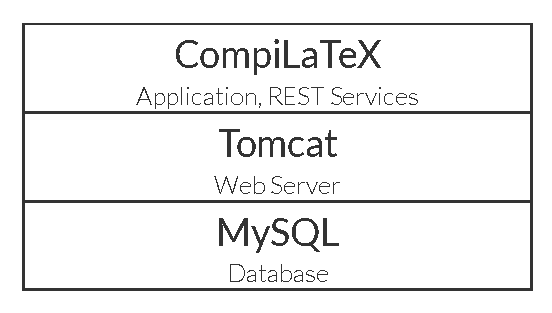
\includegraphics[width=0.5\textwidth]{images/compilatex_architecture.pdf}
	\caption{Architecture of CompiLaTeX}
\end{figure}

\pagebreak

The execution of unit tests is achieved with \name{TestNG} while integration tests make additional use of \name{RestAssured}.

For the compilation of \LaTeX files, it uses the \name{Apache Common Exec} library and requires to be run on Linux with a fully installed \name{TexLive} distribution.

\subsubsection{Model}
\label{subsubsec:compilatex-model}
There are two models for the mapping of the \LaTeX document compilation. \class{Job} is an entity that contains a collection of all document files and the name of the directory they reside. \class{JobFile} is the entity for a document file, it holds the name of the file, the parent folder, the date when it was modified last and if it is the main file, therefore to be used as target for the compilation engine.

Both entity classes have also a \name{Data Transfer Object} (\abk{DTO}{Data Transfer Object}) representation that excludes any behavior except for storage and retrieval of its own data, therefore not exposing business objects to REST services.

Operations in the persistence layer of the application are performed on DTOs exlusively, who are converted to entities before storing them in the data base. Entities are converted to DTOs vice versa when returning fetching data from the database.

\subsubsection{Services}
\label{subsubsec:compilatex-services}
The compilation of LaTeX documents is an autonomous, low-level task, involving basic file input/output operations and the execution of shell commands. Due to the fact that there are no known tools or plugins to capsulate the compilation of \LaTeX files for the Java programming language, such security critical functionality must be exposed as a service to external systems.

Hence it was implemented as a RESTful web service, providing a flexible way to compile \LaTeX \\ documents from any front-end using any technology. The distinct feature is not only its implementation, enabling the quick recompilation of marginally changed documents by updating only individual modified files or resources, but the dynamic support of \LaTeX environments.

The typical scenario for CompiLaTeX is the following: Several documents are posted to the server, then it is queried for the available compiler engines. The compilation with a given engine is requested and either the log or the \fileformat{PDF} or both can be retrieved afterwards. Before recompiling a document, the recent versions of changed files can be sent to the server and updated there. Then the document can be recompiled using the same or a different engine, requesting the log or \fileformat{PDF} afterwards.

In the following, there will be an overview given over the available REST services, ordered by resource. The presented URLs are usually prefixed with \parametertype{/rest/} but this is omitted in the following depictions for the sake of simplicity.

\headline{Latex}

The Latex resource has only a single service for the exposure of all available \LaTeX engines and is typically requested before document compilation. Since the information about the available latex compiler should be accessible at all times, they are publicly exposed.

\rest{Get Available \LaTeX Environments}
{POST}{latex/environments}
{}{APPLICATION\_JSON}
{LatexEnvironment[]}

\headline{Jobs}

The Jobs resource has multiple services for the handling of compilation jobs. Jobs can be created, updated, deleted, the compilation of a document performed. The log can be either requested as plain text or formatted with HTML elements, so can the created \fileformat{PDF} file. The log and \fileformat{PDF} can only be requested when a compilation occured beforehand, the latter even only after a success of such.

\rest{Create New Job}
{POST}{/jobs}
{}{APPLICATION\_JSON}
{JobDTO}

\rest{Compile Job}
{GET}{/jobs/\{jobId\}/compile/\{latexEnvironment\}}
{}{APPLICATION\_JSON}
{}

\rest{Get Job Log}
{GET}{/jobs/\{jobId\}/log}
{}{TEXT\_PLAIN}
{Log}

\rest{Get Job HTML Log}
{GET}{/jobs/\{jobId\}/log/html}
{}{TEXT\_PLAIN}
{String also containing HTML tags}

\rest{Get Job PDF}
{GET}{/jobs/\{jobId\}/pdf}
{}{APPLICATION\_OCTET\_STREAM}
{String}

\rest{Delete Job}
{DELETE}{/jobs/\{jobId\}}
{}{APPLICATION\_JSON}
{}

\headline{Job Files}

All services involving files need to be called with the \parameter{jobId} and \parameter{filed} as parameter, except adding a file. Both adding and updating a file consume input streams and return the resource as JSON.

To determine if a given resource resides in an outdated version on the server, the last file modification date can be requested. The response then contains the unix system time when it was last modified, therefore added or updated, on the server.

\restwithtwoparam{Add File}
{POST}{/jobs/\{jobId\}/files}
{MULTIPART\_FORM\_DATA}{}
{file}{FileInputStream}
{isMainTex}{boolean}

\restwithtwoparam{Update File}
{PUT}{/jobs/\{jobId\}/files/\{fileId\}}
{MULTIPART\_FORM\_DATA}{APPLICATION\_JSON}
{file}{FileInputStream}
{filename}{String}

\rest{Get Last File Modification Date}
{GET}{/jobs/\{jobId\}/files/\{fileId\}/lastchanged}
{}{TEXT\_PLAIN}
{JobFileDTO}

\rest{Delete File}
{DELETE}{/jobs/\{jobId\}/files/\{fileId\}}
{}{}
{no content}

\subsubsection{Implementation}
\label{subsubsec:compilatex-implementation}
The compilation of documents is organised in jobs, each having its unique directory on the server to upload files to, store logs and created PDFs. The directory name is represented by a Universally Unique Identifier (\abk{UUID}{Universally Unique Identifier}), generated upon creation of a new job and may for instance look like this: 550e8400-e29b-11d4-a716-446655440000.

When files are added or updated, input streams are read and written to the file system, in the job's directory, with the given filename. If the \parameter{jobId} URL parameter can not be mapped to a job, an error is returned in the response. Adding a file to a job also requires a parameter to indicate if it is the main \LaTeX file.

\headline{Compilation}

To compile a document, the corresponding job must contain a file being marked as main \fileformat{.tex} file. This is required to decide which file of a job is the actual target of the compilation, then achieved by using the \name{Apache Commons Exec} library which can securely and reliably execute external processes \cite{website:apache-commons-exec}.

\pagebreak

\begin{lstlisting}[language=Java, caption=Executing the Compilation of \LaTeX Files by Command Line]
/* cd to project directory */
executor.setWorkingDirectory(new File(jobDirectory));

/* build command */
CommandLine commandLine = new CommandLine(latexEnvironment.name().toLowerCase());
commandLine.addArgument("-interaction=batchmode");
Map map = new HashMap();
map.put("file", filename);
commandLine.addArgument("${file}");
commandLine.setSubstitutionMap(map);

/* execute command */
executor.execute(commandLine, resultHandler);
\end{lstlisting}

When calling the service to compile a document, a parameter is passed along, indicating which environment will be used for compilation. Prior to compilation, it is verified that this environment is actually installed on the system, returning an error in the response if it is not the case. For this, the \method{which} command is used on Linux systems.

Before compilation, the working directory is changed to the job directory. Then, the command is iteratively created, first adding the command by setting the compilation engine, then the adding parameter for the interaction mode and file name. Finally, the compilation is executed.

\headline{Log and \fileformat{PDF}}

After the compilation, both the log and \fileformat{PDF} can be requested, although the latter only after successful execution of the compilation. If so, the log or \fileformat{PDF} are read from the file system and returned. 

The process of returning the log with HTML markup is slightly more sophisticated. The log file is read into a String and searched for warnings and errors. Regular expressions will then enclose these warnings and errors with HTML markup. That way, they can later easier be styled in the front-end. And also, regular line breaks are replace by their HTML equivalent.

\headline{Available Environments}

Available \LaTeX engines for compilation are publicly exposed by REST. When requesting a list of the installed engines on the server, all values from the Enum \class{LatexEnvironment}, containing engines like \name{PDFLATEX}, \name{LUATEX}, \name{XETEX}, are fetched. Then for each is tested if it is installed on the server and added to the response. 

\pagebreak

This allows for the service to provide all \LaTeX environments dynamically, being able to add, update or remove them by installing or uninstalling their corresponding packages in the system without having to restart the server. Although this is only required when adding new engines that are not yet defined in the \class{LatexEnvironment} class. 

To avoid this slight inconvenice, it is conceivable to switch from the use of an Enum to a properties file for instance.

\subsubsection{Tests}
\label{subsubsec:compilatex-tests}

There are several unit tests in CompiLaTeX covering various aspects of the system. There are tests for the conversion between entities and DTOs, tests for the execution of the compilation by shell and tests for the persistence layer and database access.

These tests can be executed by invoking the Maven test target.

\begin{lstlisting}[caption=Invoke Unit Tests in CompiLaTex]
mvn test
\end{lstlisting}

However, this does not include the test of REST services, as they require the actual deployment of the application on a web server. The test of these services are convered by the integration tests, which can be run by invoking the following Maven target.

\begin{lstlisting}[caption=Running Integration Tests in CompiLaTex]
mvn verify
\end{lstlisting}

Integration tests simulate the actual use of a system in production mode. They assure the accurate functioning of the business logic, persistence layer, components that have already been tests in unit tests, and their flawless interaction with each other.

To deploy the application on a web server for testing purposes, two Maven plugins are used. The first, \name{failsafe} invokes the target \parameter{verify} and specifies which tests are to run.

The second controls the server by starting and shutting it down prior and posterior to the tests, specifying the port and root path. 

\pagebreak

\begin{lstlisting}[caption=Integration Tests Configuration in CompiLaTex]
<plugin>
    <groupId>org.apache.maven.plugins</groupId>
    <artifactId>maven-failsafe-plugin</artifactId>
    <version>2.17</version>
    <configuration>
        <includes>
            <include>**/*ServiceTest*</include>
        </includes>
    </configuration>
    <executions>
        <execution>
            <goals>
                <goal>integration-test</goal>
                <goal>verify</goal>
            </goals>
        </execution>
    </executions>
</plugin>

<plugin>
    <groupId>org.apache.tomcat.maven</groupId>
    <artifactId>tomcat7-maven-plugin</artifactId>
    <version>2.2</version>
    <configuration>
        <path>/</path>
    </configuration>
    <executions>
        <execution>
            <id>start-tomcat</id>
            <phase>pre-integration-test</phase>
            <goals>
                <goal>run</goal>
            </goals>
            <configuration>
                <port>9090</port>
                <fork>true</fork>
            </configuration>
        </execution>
        <execution>
            <id>stop-tomcat</id>
            <phase>post-integration-test</phase>
            <goals>
                <goal>shutdown</goal>
            </goals>
        </execution>
    </executions>
</plugin>
\end{lstlisting}

\subsection{CollaboraTeX}
\label{subsec:collaboratex}
CollaboraTeX is the web application for the collaborative editing of \LaTeX documents. It is written in Java and based on the Google App Engine platform, but runs on AppScale. That in turn is installed on OpenStack, which is utilised by the ITM Cloud Computing Lab to provide a \nameref{subsubsec:iaas}. This is illustrated in the following architecture depiction:

\begin{figure}[H]
	\centering
		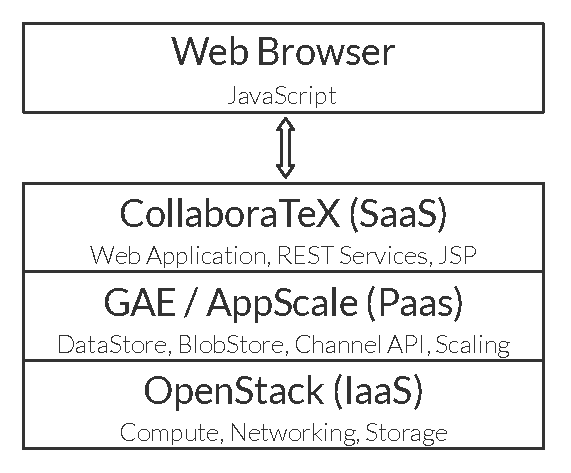
\includegraphics[width=0.5\textwidth]{images/collaboratex_architecture.pdf}
	\caption{Architecture of CollaboraTeX}
\end{figure}

CollaboraTeX makes use of lots of different Java frameworks and libraries and relies on \name{Maven} for the dependency management of them. First and foremost, the \name{AppEngine SDK} is needed to develop applications on Google App Engine. Because there are some features that are handled differently on its parallel architecture than in classic server environments, libraries for \name{DataNucleus} are also required. 

\name{DataNucleus} provides the transparent persistence of Java objects, which is here realised with JPA and EclipseLink, supporting various datastore models such as relational datastores, object-based datastores, document-based storage and more \cite{website:data-nucleus}. Before entity classes can be persisted, they must be "enhanced" by \name{DataNucleus}, which is essentially a mechanism that byte-code manipulates classes between compilation and runtime. The process itself will not be further explained, but the corresponding resources can be consulted \cite{website:data-nucleus-enhancement}.

Several of the services provided by the Google App Engine platform are used. When persisting data, they are stored in the \name{DataStore}, which has a quota of 1 megabyte and is mostly used for entities.

\pagebreak

Google describes the \name{DataStore} as:

\begin{quote}
App Engine's data repository, the High Replication Datastore (HRD), uses the Paxos algorithm to replicate data across multiple datacenters. Data is written to the Datastore in objects known as entities. Each entity has a key that uniquely identifies it. An entity can optionally designate another entity as its parent; the first entity is a child of the parent entity. The entities in the Datastore thus form a hierarchically-structured space similar to the directory structure of a file system. An entity's parent, parent's parent, and so on recursively, are its ancestors; its children, children's children, and so on, are its descendants. An entity without a parent is a root entity \cite{website:gae-datastore}.
\end{quote}

In contrast, the \name{BlobStore} is used for larger files:

\begin{quote}
The Blobstore API allows your application to serve data objects, called blobs, that are much larger than the size allowed for objects in the Datastore service. Blobs are useful for serving large files, such as video or image files, and for allowing users to upload large data files. Blobs are created by uploading a file through an HTTP request. Typically, your applications will do this by presenting a form with a file upload field to the user. When the form is submitted, the Blobstore creates a blob from the file's contents and returns an opaque reference to the blob, called a blob key, which you can later use to serve the blob. The application can serve the complete blob value in response to a user request, or it can read the value directly using a streaming file-like interface \cite{website:gae-blobstore}.
\end{quote}

\label{gae-services}
So CollaboraTeX uses the \name{DataStore} to store all entities for projects and project files, while the actual files for a \LaTeX document, also including images, the bibliography and so forth, are stored in the \name{BlobStore}.

Furthermore, a service of the Google App Engine is used that is called \name{Channel API}. It is utilised to keep persistent connections between associated clients and the application. This allows to send and receive data for document updates and synchronisation to JavaScript clients in real time \cite{website:gae-channel-api}. This technique is also known as server-push.

The search is implemented with the GAE \name{Search API} \cite{website:gae-search-api}.

\name{Jersey} is the chosen implementation of the \name{Java API for RESTful Web Services}.

For testing, \name{TestNG} and \name{RestAssured} are used, the latter for integration tests.

As \nameref{subsubsec:saas}s are commonly built as a web application that can be accessed with a simple browser, the same applies to CollaboraTeX, being most appropriate for an online \LaTeX editor. \name{Java Server Pages} are used to dynamically generate and deliver web pages based on the Hypertext Markup Language (\abk{HTML}{Hypertext Markup Language}). It integrates \name{Bootstrap} as front-end framework and makes heavy use of the library \name{jQuery} for JavaScript code \cite{website:bootstrap} \cite{website:jquery}.

\subsubsection{Model}
\label{subsubsec:collaboratex-model}
There are three models in CollaboraTeX, two to reflect \LaTeX documents and one class for the user management,  authentification and sharing.

\class{Project} is the entity that contains the name of the project and a collection of all document files. A document file again is modelled by the entity \class{ProjectFile}, it holds the name of the file, the content type, the size, the date when it was modified last and if it is the main file, to indicate it as the target for the compilation engine. Besides, the class is storing the \parameter{BlobKey} that uniquely indentifies the stored file in the BlobStore. As previously mentioned, this is necessary since the Google App Engine platform is not based on a file system. Data are stored either in the DataStore, which is mostly for persisting entities, or the BlobStore, which is used for larger files.

The \class{User} entity does contain the username, which is used to map it to LDAP services, and collections for owned projects, meaning write and read access, and accessible projects, signifying read access only.
 
All three entity classes have \name{Data Transfer Object} (DTO) representations that exclude any behavior except for storage and retrieval of its own data, to prevent the exposure of business objects via REST services.

Operations in the persistence layer are performed on \name{Data Access Objects} (DAO). They make use of the DTOs, converting them to entities before storing them in the data base. In reverse, entities are converted to DTOs before returning fetched data from the database.

\subsubsection{Services}
\label{subsubsec:collaboratex-services}
The front-end communicates with the CollaboraTeX back-end by calling its REST services, thus any actions by the user on the web page will trigger their counterparts in the back-end and change the state of the system.

A typical scenario would be this: A user logs in to the website and decides to upload an existing \LaTeX document. The files are posted to the server and a new project created, that will be displayed on the web page. When opening a \LaTeX file, a REST service is called to get the file content and display it in the editor. On changes in the document, the client will again call a service to submit them and the back-end persists the updated document state, also sending the changes to all associated clients that have the same document \LaTeX file opened. Upon compilation, everything is sent to the CompiLaTeX server and on finish, the log is requested to be displayed to the user.

The following will give an overview over the available REST services of CollaboraTeX, ordered by resource. The presented URLs are usually prefixed with \parametertype{/rest/} but this is omitted in the following depictions for the sake of simplicity.

\headline{Projects}

This resource provides multiple services for the handling of projects. They can be newly created or imported with existing files, both do not require any URL or form parameter. For the import, the files will be read from the request itself.

Projects can be renamed which requires a parameter \parameter{value} for the new name, deleted or download, all need a valid \parameter{projectId}. In the latter case, the project will be downloaded as a zipped file.

\rest{Create New Project}
{POST}{/projects}
{}{APPLICATION\_JSON}
{ProjectDTO}

\rest{Import \LaTeX Files}
{POST}{/projects/import}
{MULTIPART\_FORM\_DATA}{}
{ProjectDTO}

\rest{Download Project as ZIP File}
{GET}{/projects/\{projectId\}/download}
{}{}
{Application/ZIP}

\restwithparam{Rename Project}
{POST}{/projects/\{projectId\}/rename}
{}{APPLICATION\_JSON}
{value}{String}
{ProjectDTO}

\rest{Delete Project}
{DELETE}{/projects/\{projectId\}}
{}{}
{no content}

\headline{Project Files}

All services involving files in projects need to be called with the \parameter{projectId} and \parameter{fileId} as parameter, except getting a file upload URL, creating a new file or importing files.

There are some services being specifically for the handling of plain text files, like getting, patching and updating the file content. The difference between the two last-mentioned is that while the first changes a document by applying a patch to it, the last replaces the whole content of a text-based file. These services are needed to realise collaborative editing.

Moreover, there are services to update a file with a more recent version, renaming it, setting it as main tex file (albeit the application should be able to do an automatic detection most of the times), getting a file's meta data or deleting it.

\rest{Get File Upload URL}
{GET}{/projects/\{projectId\}/uploadurl}
{}{TEXT\_PLAIN}
{URL}

\rest{Create New File}
{POST}{/projects/\{projectId\}/files}
{MULTIPART\_FORM\_DATA}{}
{ProjectFileDTO}

\rest{Import Files}
{POST}{/projects/\{projectId\}/files/import}
{MULTIPART\_FORM\_DATA}{}
{ProjectDTO}

\rest{Get File Meta Data}
{GET}{/projects/\{projectId\}/files/\{fileId\}/meta}
{}{APPLICATION\_JSON}
{ProjectFileDTO}

\rest{Get File Content}
{GET}{/projects/\{projectId\}/files/\{fileId\}}
{}{FILE CONTENT TYPE}
{File}

\rest{Set As Main Tex File}
{POST}{/projects/\{projectId\}/files/\{fileId\}/setmaintex}
{}{APPLICATION\_JSON}
{ProjectFileDTO}

\restwithparam{Rename File}
{POST}{/projects/\{projectId\}/files/\{fileId\}/rename}
{}{APPLICATION\_JSON}
{value}{String}
{ProjectFileDTO}

\restwithparam{Patch File Content}
{POST}{/projects/\{projectId\}/files/\{fileId\}/patch}
{}{APPLICATION\_JSON}
{patch}{String}
{ProjectFileDTO}

\restwithparam{Update File Content}
{POST}{/projects/\{projectId\}/files/\{fileId\}/content}
{}{APPLICATION\_JSON}
{content}{String}
{ProjectFileDTO}    

\rest{Update File}
{PUT}{/projects/\{projectId\}/files/\{fileId\}}
{MULTIPART\_FORM\_DATA}{APPLICATION\_JSON}
{ProjectFileDTO}

\rest{Delete File}
{DELETE}{/projects/\{projectId\}/files/\{fileId\}}
{}{}
{no content}

\headline{Session}

There are session services, that are required for the synchronisation of documents in clients - and therefore enable collaborative editing in the first place.

Before a persistent connection to the client can be initiated via Channel API, it must acquire a so-called token from the server that uniquely identifies it.

To synchronise changes only with clients that have opened the same file, there are services to register and unregister for a document.

\rest{Get Channel API Token}
{GET}{/session/channel/token}
{}{TEXT\_PLAIN}
{ProjectFileDTO}

\rest{Register for an Open Document}
{POST}{/session/document/\{fileId\}/register}
{}{TEXT\_PLAIN}
{ProjectFileDTO}

\rest{Unregister for an Opened Document}
{POST}{/session/document/\{fileId\}/unregister}
{}{TEXT\_PLAIN}
{ProjectFileDTO}

\headline{Search}

The search is provided by a single service that takes a \parameter{query} as parameter and returns all found results - which are project files that matched the search criteria - as a list in JSON. 

\restwithparam{Search All Documents With Query}
{POST}{/search}
{}{APPLICATION\_JSON}
{query}{String}
{List<ProjectFileDTO>}

\subsubsection{Implementation}
\label{subsubsec:collaboratex-implementation}
Before descending into the depths of the system's implementation, the following list of features should give an idea about CollaboraTeX' functionalities:

\begin{itemize}
	\item{Creation, deletion, renaming of projects and files}
	\item{Import of existing documents and download of projects as ZIP file}
	\item{Automatic detection of \parameter{begin\{document\}} in \LaTeX files and setting them as main file}
	\item{Editor with syntax highlighting for \LaTeX}
	\item{Synchronisation of document changes for attached collaboration clients}
	\item{Immediate background persisting of document changes}
	\item{Undo and redo for local changes}
	\item{Extensive menus with most widely used \LaTeX commands}
	\item{Context menus for projects and files in the sidebar}
	\item{Keyboard shortcuts}
	\item{Inline editing of project and file names}
	\item{Search by file attributes}
	\item{Auto-completion (not only for \LaTeX commands)}
	\item{Compilation of \LaTeX files}
	\item{Viewable compilation log}
	\item{View generated \fileformat{PDF} in browser}
\end{itemize}

Hereafter, the most significant functions and their implementation details will be explained, which are \name{Import}, \name{Context Menus}, \name{Editor View}, \name{Collaboration}, \name{Compilation}, \name{Log}, \name{PDF Viewer} and \name{Search}.

%\begin{figure}[H]
%	\centering
%		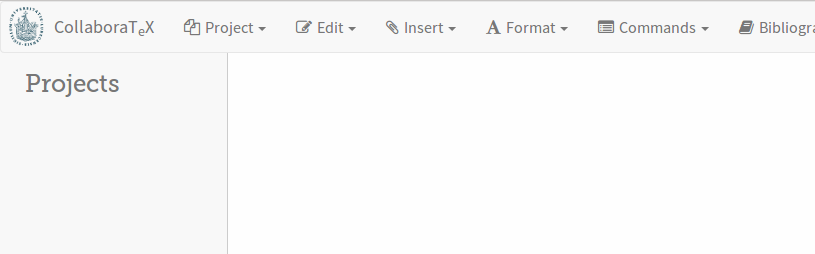
\includegraphics[width=0.8\textwidth]{images/screenshot-empty-main.png}
%	\caption{}
%\end{figure}

\headline{Import}

For the import of \LaTeX files, the front-end provides the user with a form to upload files. Files may either be selected by the filechooser or added by drag'n'drop. Files from subdirectories can be imported as well, although folders are not supported in CollaboraTeX projects because of the architecture of Google App Engine and its Blobstore (compare page \pageref{subsec:collaboratex}).

When importing a project, the project name is a required field, otherwise the form cannot be submitted. The statement of individuals that should have access to the project is an optional field. It supports autocompletion for the usernames but only as proof of concept. No user management was implemented in CollaboraTeX yet. The ultimate aim should be to aggregate the data for this by integrating the LDAP protocol.

\begin{figure}[H]
	\centering
		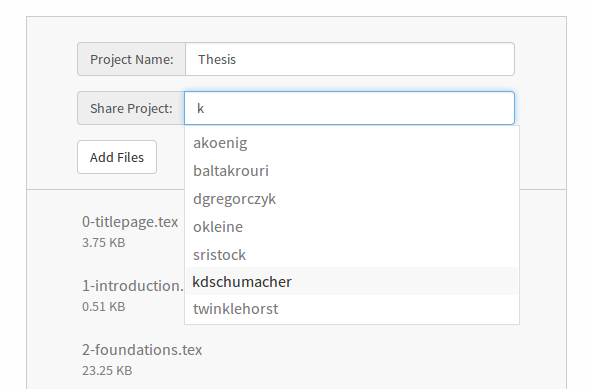
\includegraphics[width=0.66\textwidth]{images/screenshot-import-project.png}
	\caption{CollaboraTeX form to import \LaTeX documents}
\end{figure}

Upon the submit of the form, a new project is created with the given name and the files are gathered from the request. Each file is persisted in the BlobStore, added to the search index and then attached to the project, which is finally persisted itself in the DataStore.

\newpage

\headline{Context Menus}

To provide an easy and accessible way for users to control all project- and file-related actions, there are context menus for the sidebar. They  open themselves when clicking the right mouse button, are context sensible and come in three variations.

Invoking it on an empty space in the project sidebar, where projects and menus are displayed, opens a content menu that has the commands to either create a new project or import one. 

A menu with commands to share, rename, download, delete a project is openend when invoking it on a project. Additionally there are commands to create a new file or import an existing one. This is shown in the graphic below.

\begin{figure}[H]
	\centering
		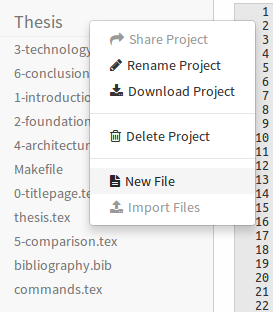
\includegraphics[width=0.35\textwidth]{images/screenshot-project-context-menu.png}
	\caption{An exemplary context menu for a project in CollaboraTeX}
\end{figure}

And then there is the context menu for files, it has options to rename a file, set it as main \TeX file or delete it.

The technical implementation for this is the following: Each item of the context menu has a unique identifier, for example:

\begin{lstlisting}[language=HTML, caption=Exemplary HTML Code for a Context Menu Item]
<li>
	<a id="newproject" class="contextmenu" tabindex="-1" href="#">
		<i class="fa fa-folder"></i> New Project
	</a>
</li>
\end{lstlisting}

For this identifier, a click handler is set in JavaScript, which performs the respective action. This handler will then execute its JavaScript code to react to the click and would typically involve a call to a REST service. \\

\begin{lstlisting}[language=JavaScript, caption=Exemplary Click Handler in JavaScript for a Context Menu Item]
$('a#newproject.menu, a#newproject.contextmenu').on('click', function() {
	$.post("/rest/projects", function(data) {
        /* create project entry in sidebar */
        createEmptyProjectList(data.id, data.name);

        /* make project name editable */
        $("a[data-pk='" + data.id + "']").editable();
        
        /* set context menu or it wouldn't be instantly available */
        setProjectContextMenu();
    });
});
\end{lstlisting}

\headline{Editor View}

The key feature of the editor view is the integrated \name{ACE Editor}. It is highlighting the syntax of a \LaTeX file, has an internal stack for redo and undo operations and features code-completion, keyboard shortcuts and much more. On the top left of the editor is a tab showing the name of the file and a button to close the editor. Also above the editor but on the right is a toolbar for the compilation. First, all available compilation engines are displayed (here PdfLaTeX) in a drop down menu, then there are buttons for the compilation, viewing the \fileformat{PDF} and the log.

\begin{figure}[H]
	\centering
		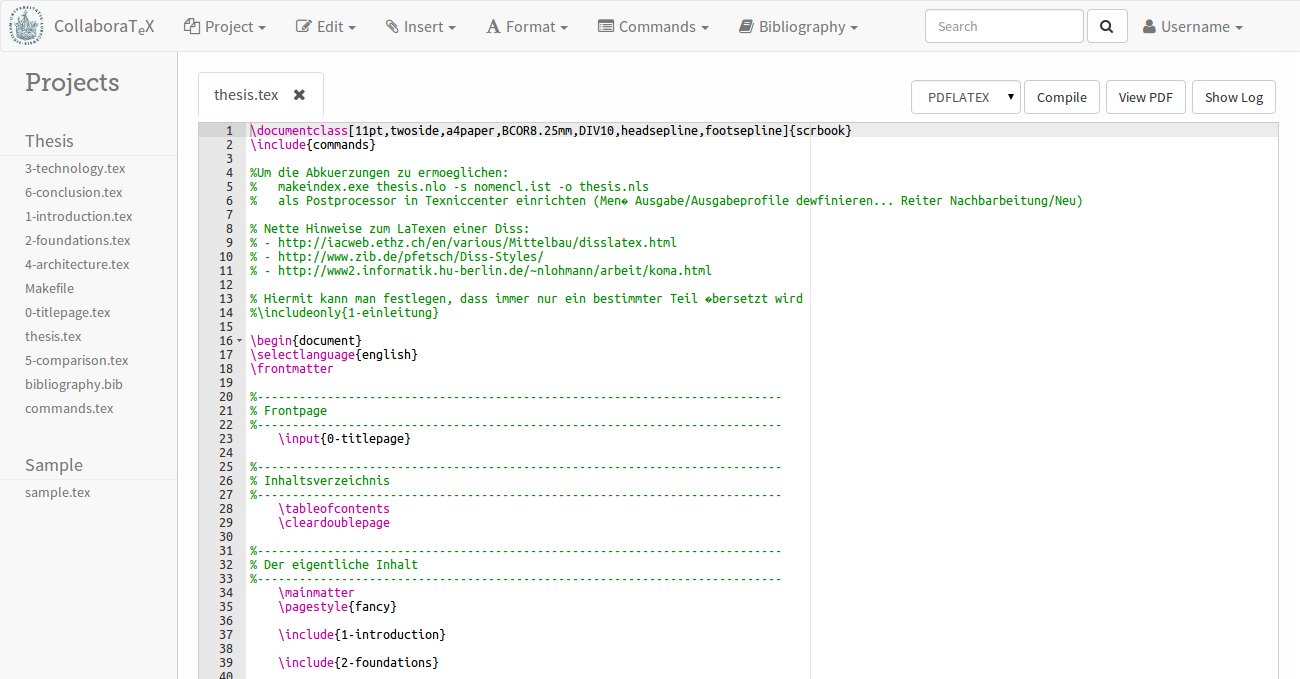
\includegraphics[width=\textwidth]{images/screenshot-editor.png}
	\caption{The editor view in CollaboraTeX}
\end{figure}

\pagebreak

A file is shown in the editor when it was clicked in the sidebar. The click handler is first checking if the main page for editor is opened and then if the chosen file is actually text-based and not in a format that could not be opened by the editor, for instance images. A service call is made to register the client for the openend document. The content of the file is then requested by calling the REST service and the response set as the editors content, displaying the file.

If the close button for the tab is clicked, a service call is made to unregister the client for the document and the editor is closed.

Undo and redo operations work only for local changes.

\headline{Collaboration}

To describe how the collaborative editing is implemented in CollaboraTeX, it will follow the typical use case of two users working together on a document at the same time. It is assumed that both users have opened the same document already and are therefore registered for it in the back-end.

To detect changes in a document, a library is used that is called jQuery Typing, developed by Maciej Konieczny \cite{website:jquery-typing}. It is rather old and straightforward, but serves its purpose. That is to detect the begin and end of a user typing. It is used here to calculate the changes and send them to the server if a user pauses his input.

\begin{lstlisting}[language=JavaScript, caption=Typing Listener for the Editor]
$('#editor > textarea').typing({
    start: function() {
        originalText = ace.edit('editor').getSession().getValue();
    },
    stop: function() {
        var patch = getPatch(originalText);
        sendChangesToServer(patch);
    },
    delay: 400
});
\end{lstlisting}

So when a user starts to type, the content of the editor is saved in a global variable \parameter{originalText}. If the typing is then paused for at least 400 milliseconds, the user is thought to have ended his input. First, a patch of the document changes based on the stored original content is calculated and then sent to the server.

For the all text-related operations that are the base for \nameref{subsubsec:operational-transform}, such as creating diffs and patches, the \name{Google Diff Match Patch} library is used in JavaScript.

\pagebreak

\begin{lstlisting}[language=JavaScript, caption=Creation of a Diff and subsequently a Patch for the Document's Changes]
function getPatch(originalText){
	var dmp = new diff_match_patch();

	/* calculate diff from original and current text */
	var currentText = ace.edit('editor').getSession().getValue();
	var diff = dmp.diff_main(originalText, currentText, true);

	/* make patch from diff and original and current text */
	var patch_list = dmp.patch_make(originalText, currentText, diff);
	var patch = dmp.patch_toText(patch_list);

	return patch;
}
\end{lstlisting}

The patch is then passed to a function not cited here, that gathers the \name{projectId} and \name{fileId}. Finally the patch is posted to the REST resource.

\begin{lstlisting}[language=JavaScript, caption=Posting the Patch to the REST Service]
function patchFileContent(projectId, fileId, patch) {
    $.post('/rest/projects/' + projectId + '/files/' + fileId + '/patch', {patch: patch}, function(data) {
        /* not much to do on success */
    });
}
\end{lstlisting}

After the server receives the patch, it first fetches the \class{Project} object with the given \parameter{projectId} and then the \class{ProjectFile} object for the given \parameter{fileId}. On the server, the same library is used as in the client, \name{Google Diff Match Patch}, which is important to achieve not only the synchronisation between clients but also across all clients and the server.

To possess the most recent version of the document on the server then amounts to the easy task of applying the patch on the current state of the document as the server knows it.

\begin{lstlisting}[language=Java, caption=Applying the Patch for a Document on the CollaboraTeX Server]
private String createPatchedContent(String patch, String content) throws IllegalArgumentException {
    /* create diff match patch instance */
    diff_match_patch dmp = new diff_match_patch();
    
    /* create single patches from text patch and apply to file content */
    List<Patch> patches = dmp.patch_fromText(patch);
    Object[] results = dmp.patch_apply((LinkedList<Patch>) patches, content);
    
    /* first array entry contains patched text  */
    return (String) results[0];
}
\end{lstlisting}

As there is no possibility to update files that are stored in the BlobStore, the old version of the file is deleted from it first, then the new patched version is written to the BlobStore and all references in the \class{ProjectFile} object are updated, such as the \parameter{blobKey} and \parameter{lastChanged} date. This ensures that all changes to the document are persisted immediately.

The search index however is able to update existing data, so the new file is simply put to it and the index updated accordingly.

The last and maybe most important step is that the changes are broadcasted to all clients that are currently editing the same document. This is achieved by using the Google App Engine Channel API, thus implementing a server push where the web server leaves a connection open to send out data on events to the client immediately \cite{burke2013restful}. 

These connections are created on the client-side when a user accesses the website, their lifetime is two hours.

\begin{lstlisting}[language=Java, caption=Broadcast Changes to All Associated Clients Having the Same Document Opened]
private void pushPatchToAllAssociatedClients(Long fileId, String patch, String originSessionId) {
        
        /* get map of all opened documents */
        Map<String, Long> openedDocuments = SessionManager.getOpenedDocuments();
        for (Entry<String, Long> entry : openedDocuments.entrySet()) {
            
            /* get session and document id */
            String sessionId = entry.getKey();
            Long documentId = entry.getValue();
            
            /* send patch to client if it has opened the same file and was NOT the one who made the changes */
            if (documentId.equals(fileId) && !sessionId.equals(originSessionId)){
                channelService.sendMessage(new ChannelMessage(sessionId, patch));
            }
        }
    }
\end{lstlisting}

The Channel API declares standard functions in JavaScript that are executed on the client-side when receiving any data from the server. Those are \method{onOpen}, \method{onMessage}, \method{onError} and \method{onClose}. 

Here the \method{onMessage} function is used to receive and process the message from the server containing the patch.

\pagebreak

\begin{lstlisting}[language=JavaScript, caption=Apply the Broadcasted Patch From the Server on the Client]
function onMessage(patch) {
    if ($('#editor')) {
        var dmp = new diff_match_patch();

        /* apply patch to current editor content */
        var currentText = ace.edit('editor').getSession().getValue();
        var patches = dmp.patch_fromText(patch.data);
        var results = dmp.patch_apply(patches, currentText);

        /* set patched content as new content */
        ace.edit('editor').getSession().setValue(results[0]);
    }
}
\end{lstlisting}

\label{simpler-ot-reason}

When comparing this approach to the pure theory of \nameref{subsubsec:operational-transform} it strikes the eye that this implementation is a simpler version of it. It does not take into account that the transit time of messages between clients and server, while two or more users edit the document in real-time, can lead to conflicts, as updates can be outdated by the time they will either reach the server or the client.

This is due to two major reasons: On the one hand, it is assumed that delay of messages, high transit times or even loss of connection are ruled out in the target environment, the ITM Cloud Computing Lab. 

On the other hand, the lack of \nameref{subsubsec:operational-transform} libraries that can be used with a Java back-end makes it neccessary to write the logic behind it from scratch. Given the time and scope of this work, this proved to be unfeasible.

\headline{Compilation}

The compilation is triggered from the toolbar above the editor. When opening the editor, a request to a CompiLaTeX REST service is made to get the available compilation engines and display them as a drop down menu (compare page \pageref{subsubsec:compilatex-services}). 

The toolbar also provides buttons for the compilation, to view the \fileformat{PDF} and the log. In case of non-reachability of the CompiLaTeX server, a hint that compilation is currently not possible is shown instead of the toolbar.

The communication and interaction among both servers can be seen in the graphic below. To create no interdependencies between them, all service calls are made by JavaScript in the client. However, they could directly communicate with each other on the application layer by consuming their REST services.

\begin{figure}[H]
	\centering
		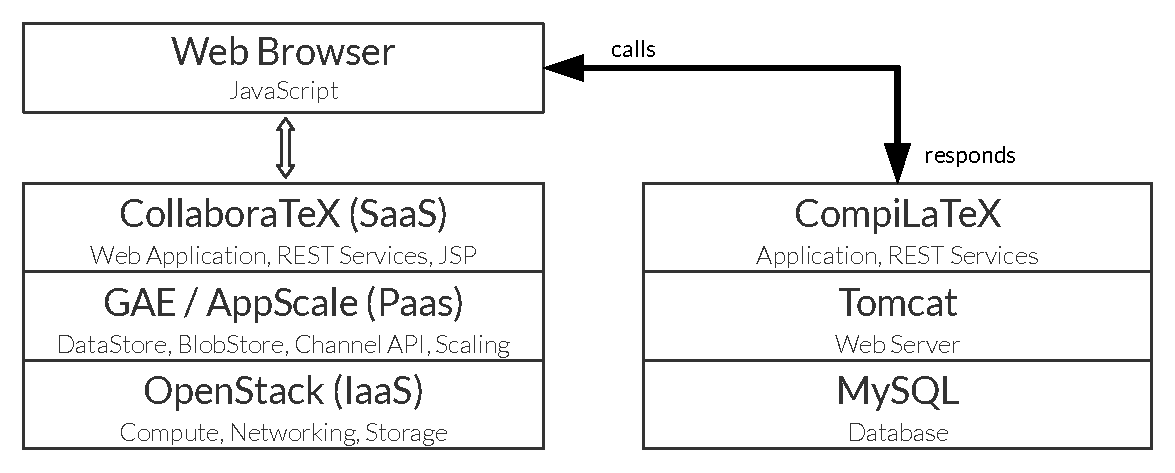
\includegraphics[width=\textwidth]{images/cotex_architecture.pdf}
	\caption{Interaction between CollaboraTeX and CompiLaTeX}
\end{figure}

When triggering the compilation, the following things happen throughout the process. Initially, a service call is made to CompiLaTeX to create a new job. Then all files are gathered and posted by the function \method{addFile} to the recently created CompiLaTeX compilation job. 

When all files were transfered to the CompiLaTeX server, the compilation can be invoked by yet another service call with the parameters \parameter{jobId} and the chosen \parameter{latexEnvironment}. Upon completion, the log for the job is requested and appended to a div the CollaboraTeX webpage, as well as the compilation time is displayed right next to the toolbar.

\begin{lstlisting}[language=JavaScript, caption=Click Listener for the Compilation Button in CollaboraTeX]
/* get latex environment for compilation from select */
var latexEnvironment = $('#latexenvironment option:selected').text();
/* create job by posting to CompiLaTeX service */
var job = createNewJob();

/* get project files */
var projectId = getProjectIdFromTab();
var fileIDs = getProjectFileIDsFromSidebar(projectId);
for (var i = 0; i < fileIDs.length; i++) {
	/* add them to CompiLaTeX Job by posting to its service */
    var fileId = fileIDs[i];
    var fileMetaData = getFileMetaData(projectId, fileId);
    var content = getFileContent(projectId, fileId);
    var createdFile = addFile(job.id, content, fileMetaData.name, fileMetaData.mainTex);
}

/* compile and append log to div#log*/
compileJob(job.id, latexEnvironment);
appendLogToPage(getHtmlJobLog(job.id));
\end{lstlisting}

How the compilation is achieved in CompiLaTeX is described in \nameref{subsubsec:compilatex-implementation} on page \pageref{subsubsec:compilatex-implementation}.

\headline{Log}

As previously mentioned, the log is appended to a collapsible div after compilation. It can be shown or hidden by clicking the corresponding button in the compilation toolbar above the editor.

The log is presented in a webpage-optimised way, meaning that errors and warnings that occured during the compilation are coloured in red, respectively yellow, throughout the log to let the user spot them more easily. Their number of occurrences is also summarised in the headline.

\begin{figure}[H]
	\centering
		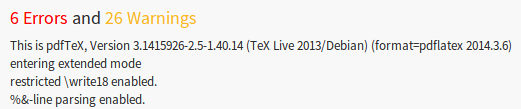
\includegraphics[width=0.66\textwidth]{images/screenshot-compile-log-warning.png}
	\caption{Log for erroneous compilation with coloured errors and warnings}
\end{figure}

If the compilation went well, so no errors occured and the output (\fileformat{PDF}) could be successfully created, the most important information are summarised in the headlines of the log, showing the filename, number of pages and filesize.

\begin{figure}[H]
	\centering
		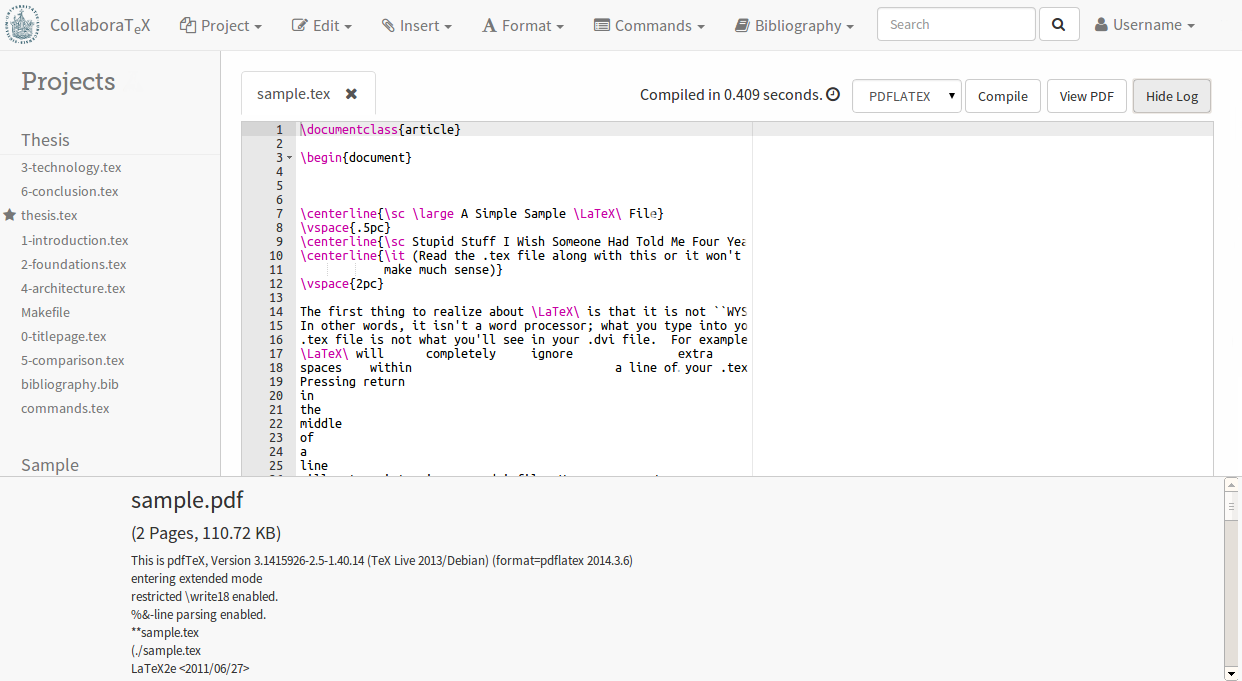
\includegraphics[width=\textwidth]{images/screenshot-compile-log-success.png}
	\caption{Log for successful compilation with summarised document information}
\end{figure}

\pagebreak

\headline{PDF Viewer}
\label{pdf-viewer}

To allow users to quickly see the generated document, \name{PDF.js} is embedded into CollaboraTeX, a \fileformat{PDF} viewer written in JavaScript which describes itself as a "web standards-based platform for parsing and rendering PDFs" \cite{website:pdf-js}.

Integrating it has multiple advantages. To begin with, it allows the operating system independent view of \fileformat{PDF} files, as it is uncertain which operating system a user of the online \LaTeX editor might use and if it has an installed \fileformat{PDF} application. Secondly, it is easier for the user to instantaneously display the file in the browser than having him to download and open it with a native application.

PDF.js is localised for various languages and offers rich and extensive features to view \fileformat{PDF}s. The page previews can be seen in a hideable sidebar, there is a search function, jump to page, zooming, fullscreen view, printing and bookmark support and the file can directly be saved.

How the \fileformat{PDF} view looks like can be seen from the following sample document:

\begin{figure}[H]
	\centering
		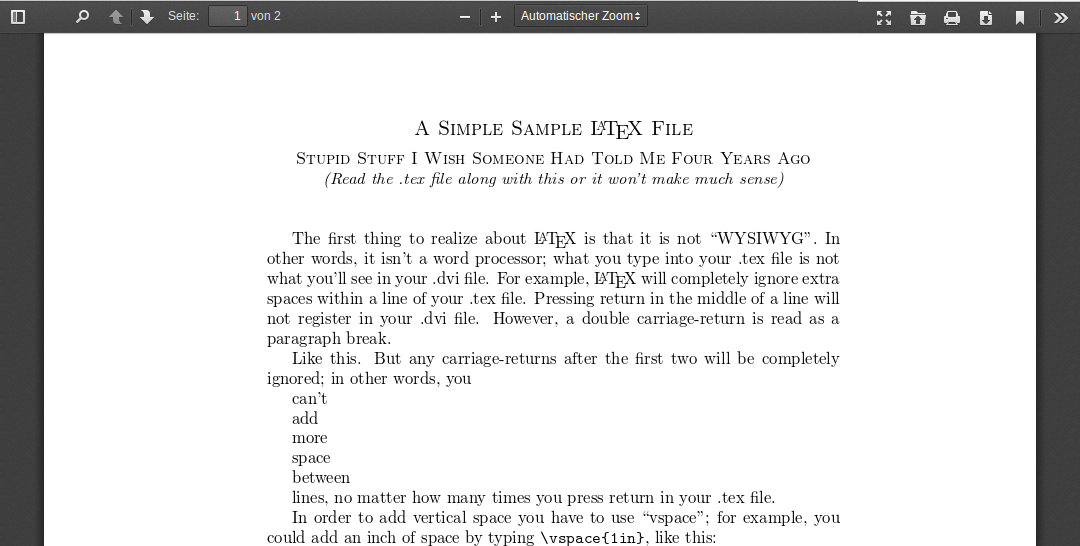
\includegraphics[width=\textwidth]{images/screenshot-pdf-viewer.png}
	\caption{Embedded \fileformat{PDF} viewer in CollaboraTeX}
\end{figure}

\headline{Search}

The search is realised with the Google App Engine \name{Search API} \cite{website:gae-search-api}. It provides a model for the indexing of documents that contain structured data and persists them in a store that is optimised for search operations. While the number of documents in such an index is unlimited, the search cannot return more than 10,000 matches. Nevertheless, this is more than sufficient for the needs of this \LaTeX editor.

Entries are represented in the search index as documents. To add files to the search index, a document must be build. Such a document can have fields with different primitive values like text, a number, a date, a locale. The fields are here populated with the file's attributes, as the code excerpt shows below. After creation, the document can be added to the search index.

\begin{lstlisting}[language=Java, caption=Building a Document Entry for the Search Index]
Document newDoc = Document.newBuilder().setId(String.valueOf(fileDTO.getId()))
    .addField(fb.setName("key").setText(fileDTO.getKey().getId()))
    .addField(fb.setName("blobKey").setText(fileDTO.getBlobKey()))
    .addField(fb.setName("name").setText(fileDTO.getName()))
    .addField(fb.setName("contentType").setText(fileDTO.getContentType()))
    .addField(fb.setName("size").setText(fileDTO.getSize()))
    .addField(fb.setName("lastChanged").setText(fileDTO.getLastChanged()))
    .addField(fb.setName("mainTex").setText(fileDTO.isMainTex())).build();

IndexSpec indexSpec = IndexSpec.newBuilder().setName("IndexName").build();
Index index = SearchServiceFactory.getSearchService().getIndex(indexSpec);
index.put(document);
\end{lstlisting}

When a user now uses the search functionality in the front-end, the query is posted by Java-Script to the according CollaboraTeX REST service and executed on the search index. To retrieve results from the search index, a simple method call is sufficient.

The results are returned as a list. For each document in it, the fields are re-mapped and a \class{ProjectFile} object is constructed. This is then added to a list of found files, finally returning it as JSON response to the client.

\begin{lstlisting}[language=Java, caption=Retrieving Results from the Search Index for a Query]
Results<ScoredDocument> results = SearchIndexManager.INSTANCE.retrieveDocuments(query.trim());
/* get attributes for each found document */
for (ScoredDocument document : results) {
    Key key = KeyFactory.createKey(document.getField("key").getText());
    BlobKey blobKey = new BlobKey(document.getField("blobKey").getText());
    String name = document.getField("name").getText();
    String contentType = document.getField("contentType").getText();
    long size = document.getField("size").getText();
    long lastChanged = document.getField("lastChanged").getText();
    boolean mainTex = document.getField("mainTex").getText();

    /* create file dto and add to found list */
    ProjectFileDTO fileDTO = new ProjectFileDTO(blobKey, name, contentType, size, lastChanged, mainTex);
    fileDTO.setKey(key);
    foundFiles.add(fileDTO);
}
return Response.ok().entity(foundFiles).build();
\end{lstlisting}

Upon reception of the results in the client, all found matches will be displayed in a table to the user. The number of matches and the performed query are both stated in the headline. The list itself is containing the different file attributes name, content type, filesize, date of last modification and if the file is set as main \TeX file.

\begin{figure}[H]
	\centering
		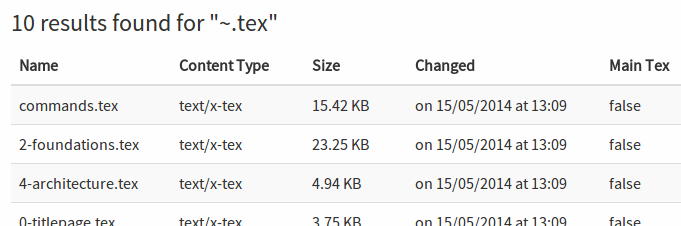
\includegraphics[width=0.8\textwidth]{images/screenshot-search.png}
	\caption{Search results are displayed in a table in CollaboraTeX}
\end{figure}

\label{reason-no-full-text-support}
As can be seen, the search does not yet provide full-text support. Although it would require minor effort to implement it, the way in which the search index is implemented on Google App Engine would pose a problem to the task of both providing the possibility to search a file's contents and its attributes. This is, that such an additional field for the content of a document has to be a Null value for non-text content types.

The full-text search is not considered to be of such importance that the examination of this problem was a priority and remained lastly unimplemented.

\subsubsection{Tests}
\label{subsubsec:collaboratex-tests}

Unit testing covers methods of a class and is used to assure their correct functioning. They are here utilised to test the conversion between entities and DTOs and the  access to the persistance layer by using Data Access Objects. These unit tests can be executed by invoking the Maven test target.

\begin{lstlisting}[caption=Invoke Unit Tests in CollaboraTeX]
mvn test
\end{lstlisting}

As the unit tests cover only basic and simple functionalities, more in-depth application tests are needed to be performed in a different way. The test of REST services requires the actual deployment of the application on a web server and are covered by the integration tests, which can be run by invoking the following Maven target.

\begin{lstlisting}[caption=Running Integration Tests in CollaboraTeX]
mvn verify
\end{lstlisting}

The integration tests are used to simulate the behaviour of the application in production mode. When using them, not only the flawless functioning of business logic, persistence layer and components that have already been unit-tested is ensured, also their interaction with one another is. 

To deploy the application for testing purposes on a Google App Engine development server, two Maven plugins need to be configured. The first, \name{failsafe} invokes the target \parameter{verify} and specifies which tests are to run. The second plugin has the task to control the start and shutdown of the server. It does so prior and afterwards to the tests.

\begin{lstlisting}[caption=Integration Tests Configuration in CollaboraTeX]
<plugin>
    <groupId>org.apache.maven.plugins</groupId>
    <artifactId>maven-failsafe-plugin</artifactId>  
    <version>2.17</version>  
    <configuration>  
        <includes>  
            <include>**/*ServiceTests.java</include>
        </includes>  
    </configuration>  
    <executions>
        <execution>  
            <phase>integration-test</phase>
            <goals>  
                <goal>integration-test</goal>  
                <goal>verify</goal>
            </goals>  
        </execution>  
    </executions>  
</plugin>

<plugin>
    <groupId>com.google.appengine</groupId>
    <artifactId>appengine-maven-plugin</artifactId>
    <version>${appengine.version}</version>
    <executions>
        <execution>
            <phase>pre-integration-test</phase>
            <goals>
                <goal>devserver_start</goal>
            </goals>
        </execution>
        <execution>
            <phase>post-integration-test</phase>
            <goals>
                <goal>devserver_stop</goal>
            </goals>
        </execution>
    </executions>
</plugin>
\end{lstlisting}

\pagebreak




	\chapter{Conclusion}
To conclude this work, its outcome is reflected and structured into the following subchapters. Starting with the \nameref{sec:work-insights} which describes major problems and findings during its development, it is succeeded by the functionalities which were ultimately implemented and which were not. 

The last and final remarks apply for the outlook of further potential implementations and works.

\section{Insights of the work in hand}
\label{sec:work-insights}
Starting this work, research was conducted about the basic principles of collaboration of invidials and specifically the algorithms, design patterns and framework and library encapsulating such functionality.

Additionally, it was attempted to find out if there are pre-exisiting solutions that are dedicated to provide a \LaTeX editor that can be used collaboratively in real-time and allows the self-hosting on one's own infrastructure.

Both investigations for collaboration libraries and editors lead to the initial insight that \name{Node.js} is the currently leading platform for collaborative solutions. This is due to its nature as light\-weight, asynchronous web server that excels for thousands of concurrent connections.

The \nameref{subsubsec:operational-transform} libraries \name{TogetherJS}, \name{OT.js} and \name{ShareJS} are all based on Node.js, as well as the plain-text editors with integrated collaboration features \name{FirePad} and \name{Etherpad}. The same applies for the, at the time of the inception of this work, solely known \LaTeX editor \name{\nameref{subsec:flylatex}}.

As the \nameref{subsec:technical-constraints} and \nameref{subsec:software-requirements} of the designated users in the Institue of Telematics were identified, a thought was to simply extend the \name{\nameref{subsec:flylatex}} editor to provide the desired functionalities. Yet it was immediately ruled out as even the most basic functions were not providing a satisfactory user experience, leading to the belief that it made more sense to re-implement such an collaborative \LaTeX real-time editor from scratch.

The other major reason was the wish to compare the performance of Node.js with an other true and established Cloud Computing technology.

\pagebreak

For this purpose, the implementation in \name{Java}, based on the \name{Google App Engine} platform and \name{AppScale} was chosen. The downside of this approach was the apparent lack of \nameref{subsec:collaborative-editing-approach} libraries and support in Java. It was eluded by the use of \name{Google Diff Match Patch}, a \nameref{subsubsec:operational-transform} library, the consequence being that the sychronisation sequence and message exchange between clients using the \LaTeX editor had to be self-implemented. Albeit the final implementation is a simpler version of the \nameref{subsubsec:operational-transform} approach: It applies document updates on the server only and then broadcasts it to the clients, assuming that delay of messages is ruled out in the target environment, the ITM Cloud Computing Lab (compare chapter \ref{simpler-ot-reason}). Given the time and scope of this work, a more sophisticated solution proved to be unfeasible.

Halfway through this work however, there was a caesura. They previously only as website operated \name{\nameref{subsec:sharelatex}} that required subscriptions for its extensive services, went open source  \cite{website:sharelatex-oss}. Compare chapter \ref{subsec:sharelatex} for the reasons behind their decision. Although \nameref{subsec:sharelatex} is more well-engineered than the previously cited alternative and provides a better user experience, the implementation was continued nevertheless. For one reason, to create a custom-tailored solution for the ITM Cloud Computing Lab that focused on slightly different aspects. For another reason, the performance comparision could be conducted in the same way, as this solution is also based on Node.js. And for the last reason, the author of this work was eager to achieve at least the creation of a collaborative \LaTeX editor that was of equal value.

The decision was made to develop two different servers. One that provides the compilation of \LaTeX documents, called \name{\nameref{subsec:compilatex}}, and one for the user front-end with the editor \name{\nameref{subsec:collaboratex}}. Their respective architecture, its data model, an overview of their services, and a detailled walkthrough of their implementation and tests are described in chapter \ref{chap:architecture}.

During the implementation, the complexity of architecture and the integration of different technologies proved to be a main effort for both servers, fighting especially with configuration and to a lesser extent also programming errors. Once the foundation was layed, the development happened test-driven and progressed rather fast by the assistance of regression tests.

Google App Engine proved to be quite suitable for the needs of a collaborative \LaTeX editor, especially with its services described in chapter \nameref{gae-services}. Besides handling entities in the \name{DataStore} and larges files in the \name{BlobStore}, there is a \name{Search API} to provide search functionality and a \name{Channel API} to manage persistent connections to clients. The only negative impact was the absence of a direct access to the file system, Google App Engine has no such thing due to its shared and parallel nature. This lead to the constraint that projects in \nameref{subsec:collaboratex} cannot contain subfolders as the mapping would constitute a relatively complex issue.

The same suitability also holds true for the integrated \name{Ace Editor} and \name{Google Diff Match Patch} library (compare chapter \nameref{subsec:collaboratex}).

What proves to be a problem however are the changing releases of OpenStack. When a server is shutdown, it is usually sufficient to simply rejoin all services. But with the provided OpenStack test server, things are a bit different as it has CentOS 6.5 installed as operating system.

The whole installation must be re-run, for which the current release is downloaded. As the current releases might not match the release that was actually installed on the server, it may lead to problems with package dependencies and various other things in a lot of times. \cite{website:openstack-releases}

This also happened during this work, as the latest release changed from the pre-installed \name{Grizzly} to the \name{Icehouse} release, see the OpenStack release page. \cite{website:openstack-releases} It led to problems with Python packages - which seems to be a particular problem of the DevStack installation, used for the OpenStack server at hand - and eventually to the omission of a comparison between the platforms of both the existing \LaTeX editors and the one developed in this work, \name{Node.js} and \name{Google App Engine}, in terms of scalability and performance.

For to the productive use of the \LaTeX editor, it would be recommended to use a regular OpenStack installation as opposed to the development version.

\section{Implemented Functionalities}
\label{sec:implemented-functionalities}
As the success of this work is largely based on the effective realisation of the majority of \nameref{subsubsec:functional-requirements} while giving regards to the \nameref{subsubsec:implicit-requirements}, their successful implementation is noted in the following.

Out of 21 functionalities, 12 could could be implemented, among them the all five from the group of \nameref{tab:high-priority} and two thirds of those with medium priority. Of the \nameref{tab:low-priority}, three were completed. The arithmetic average for their rating is 7.4 and the median 7.6 for them.

\begin{table}[H] % \todo{vor Druck ändern -> h!}
	\begin{center}
		\footnotesize
		\setlength\extrarowheight{5pt}
		\rowcolors{1}{}{lightgray}
		\begin{tabular}{ p{11cm} cp{1.5cm} }
		  	\textbf{Functionality} 	  														& \textbf{Rating} \\
			\hline
			Undo/Redo of edits																& 8.7 \\
			Support of bibliography/BibTeX management										& 8.3 \\
			Viewable log of the compilation													& 8.3 \\
			Automatic background save while editing (e.g. every five minutes)				& 8.1 \\
			Tabs for multiple opened documents and parallel editing							& 8.0 \\
			\hline
			Download of single files/the whole project										& 7.8 \\
			Import function for existing \LaTeX projects									& 7.3 \\
			Code completion similiar to an IDE												& 7.1 \\
			Download of single files/the whole project										& 7.0 \\
			\hline
			Toolbar for the most common commands (bold text, section, figure et cetera)		& 6.1 \\
 			Capability to print documents													& 6.1 \\
			Collection of formulas, extended commands, symbol tables						& 5.7 \\
		\end{tabular}
		\caption{Implemented functionalities}
	\end{center}
\end{table}

\pagebreak

On the contrary, nine features were left partially or fully unimplemented. Only two \nameref{tab:medium-priority} could not be accomplished, the vast majority of seven functionalities is however made up of those with low priority. \\ They have an average mean rating of 5.4 which is significantly lower than for their counter-parts, the implemented functionalites from above, and a median of 6.1.

\begin{table}[H] % \todo{vor Druck ändern -> h!}
	\begin{center}
		\footnotesize
		\setlength\extrarowheight{5pt}
		\rowcolors{1}{}{lightgray}
		\begin{tabular}{ p{11cm} cp{1.5cm} }
		  	\textbf{Functionality} 	  														& \textbf{Rating} \\
			\hline
			Full-text search over all documents												& 7.6 \\
			Notifications on changes made by other users or their activities				& 7.1 \\
			\hline
			Rights management for documents (not accessible for others, share with user)	& 6.5 \\
			Preview of the document as parallel view of \LaTeX and \fileformat{PDF}			& 6.5 \\
			Existing logins can be used (authentification by LDAP)							& 6.1 \\
			Personalised settings of editor appearance (font size, theme and so on)			& 6.0 \\
			Bookmarks/markers can be set in documents				 						& 5.3 \\
			\LaTeX templates to follow the ITM conventions									& 5.0 \\
			Syntax highlighting for other languages except \LaTeX							& 4.2 \\
		\end{tabular}
		\caption{Unimplemented functionalitites}
		\label{unimplemented-functionalitites}
	\end{center}
\end{table}

The full-text search is not yet fully implemented, as explained in chapter \nameref{reason-no-full-text-support}, because it was not considered to be of such importance to solve the related problems in the short time of this work. What was implemented however, was a basic search for project files and their attributes such as name, size, content type and so forth.

All features regarding the user management were also left unimplemented, such as notifications, rights management, LDAP logins, personalised settings. It was decided that the integration of this would require major effort and a vast time budget that would be at the expense of other important functionalities that were prioritised higher.

While the preview of the document as parallel view of \LaTeX and \fileformat{PDF} was not accomplished, a \fileformat{PDF} viewer was integrated very well (compare chapter \ref{pdf-viewer}). The solution, opening a document in a new browser tab, could easily be reconstructed to achieve the parallel view. But for reasons of better accessibility of both the editor and the viewer, it was decided to leave them as independent components.

All other functionalities, bookmarks, templates and syntax highlighting for other languages, were simply ignored due to insufficient significance to the users.

At last, there is one feature missing that was valued of major importance and regarded as indispensable: Document changes should be backed by the usage of a version control system. As the way in which Google App Engine operates with files is rather unique, it lead to a rather extensive problem how to obtain files from the \name{BlobStore} and put them under version control. Given the time limitation of this work, this concern was eventually not addressed.

\section{Outlook}
\label{sec:outlook}
Contemplating about future capabilities and developments regarding this \LaTeX online editor, what first comes to mind are the \nameref{unimplemented-functionalitites}. But beyond that, there are endless possibilities of additional features that would enrich not only this editor but also the way in which a user perceives its use.

\begin{itemize}
	\item The compilation of \LaTeX files could be executed with \name{latexmk}, just as in \nameref{subsec:sharelatex}, resulting in quicker and easier compilation.
	\item Easier configuration and deployment of the \name{CompiLaTeX} and \name{CollaboraTeX} server by loading their start-up parameter such as port, URL, available \LaTeX engines by XML or properties file.
	\item The spellchecking of documents could be supported in various languages by extending the used \name{Ace Editor}.
	\item Inline references in the editor for \LaTeX packages and commands with a brief explanation of them in a pop-up.
	\item Missing \LaTeX packages could be automatically downloaded by the \name{CompiLaTeX} server and added to the project directory to re-compile the document successfully.
	\item Wrong paths of included files or images could be detected prior to compilation and a warning issued that there are missing references.
	\item Retrieval of the supported \LaTeX packages on the \name{CompiLaTeX} server by RESTful web service.
	\item Better analysis of the compilation result and abolition of the \parameter{-interaction=batchmode} parameter, instead the user will be notified of compilation errors and can decide how to proceed.
\end{itemize}

It is imaginable that this editor will be developed further in other thesis or case studies at the University of Lübeck, which also leads to the issue of publication: At the moment, this work is still being hosted by the private Git repository of the Institute of Telematics, but it is planned to release it as free and open source software for the common public interest. A relocation to a GitHub repositiory might therefore be in the best interest of all persons involved. In addition to it, the necessary licence for the publication must also be resolved.

Furthermore, it will be interesting to observe how Google will continuously evolve the Google App Engine platform and how its functions and capability will progress.

This applies even more for the nowadays increasingly smarter and comprehensive collaboration libraries, with \name{TogetherJS} parading the ever-growing opportunities. It is the first library to integrate messaging and audio chat while only requiring the inclusion of a single JavaScript snippet (compare page \pageref{together-js}).



%---------------------------------------------------------------------------
% Anhang
%---------------------------------------------------------------------------
	\appendix

		\listoffigures

	    \listoftables
		
		\lstlistoflistings
		
		%---------------------------------------------------------------------------

    %using: \abk{Abk.}{Abk�rzung}
		\cleardoublepage
		\phantomsection
		\printnomenclature
		\addcontentsline{toc}{chapter}{\nomname}

	%prevent linebreaks in bibliography
		\interlinepenalty=10000

		\bibliographystyle{acm}
		\bibliography{bibliography}

    	\printindex

\end{document}
